\documentclass[aspectratio=169,11pt,t]{beamer}
%\def\WITHNOTES{}   % <- uncomment for slides + speaker notes on second screen
% ================= shared look (AI-Driven Automation series) =================
% ============================================================
% AI-Driven Automation -- shared Beamer look (Prof. Dr. C. Weisser, HSBI)
% ------------------------------------------------------------
% Speaker notes: every frame carries \note{...}.
%   * Slides only (default): compile as is.
%   * Slides + notes on a second screen (for Presentation.app / pdfpc):
%       uncomment the line  \def\WITHNOTES{}  at the very top of the file
%       (or compile with:  pdflatex "\def\WITHNOTES{}\input{<file>}")
% Fonts/packages: Fira Sans, Fira Mono, fontawesome5, tcolorbox, tikz
%   (all part of TeX Live / MacTeX / Overleaf).
% ============================================================

% ---------- Encoding, language, fonts ------------------------
\usepackage[utf8]{inputenc}
\usepackage[T1]{fontenc}
\usepackage[english]{babel}
\usepackage[sfdefault,lining]{FiraSans}
\usepackage[scale=0.86,lining]{FiraMono}
\usepackage{textcomp}

% ---------- Core packages ------------------------------------
\usepackage{graphicx}
\usepackage{booktabs}
\usepackage{tabularx}
\usepackage{array}
\usepackage{amsmath,amssymb}
\usepackage{xcolor}
\usepackage{hyperref}
\usepackage{listings}
\usepackage{fontawesome5}
\usepackage{tikz}
\usetikzlibrary{arrows.meta,positioning,calc,fit,backgrounds,shapes.geometric,shapes.misc,decorations.pathreplacing}
\usepackage[most]{tcolorbox}
\usepackage{pgfpages}
\usepackage[kerning=true]{microtype}
\DisableLigatures[-]{encoding = *, family = tt* }   % keep "--" as two hyphens in code
\frenchspacing

% ---------- Speaker-notes switch -----------------------------
\ifdefined\WITHNOTES
  \setbeameroption{show notes on second screen=right}
\fi

% ---------- Colour palette -----------------------------------
\definecolor{cNavy}{HTML}{0F2A44}
\definecolor{cInk}{HTML}{1E2A36}
\definecolor{cBlue}{HTML}{1F6FB2}
\definecolor{cBlueL}{HTML}{E3EEF8}
\definecolor{cTeal}{HTML}{0E8C7F}
\definecolor{cTealL}{HTML}{DDF1EE}
\definecolor{cOrange}{HTML}{D9731A}
\definecolor{cOrangeL}{HTML}{FBEBDC}
\definecolor{cRed}{HTML}{B42318}
\definecolor{cRedL}{HTML}{FBE4E1}
\definecolor{cPurple}{HTML}{6E4BA8}
\definecolor{cPurpleL}{HTML}{ECE6F6}
\definecolor{cGreen}{HTML}{2E7D32}
\definecolor{cGreenL}{HTML}{E1F1E2}
\definecolor{cGray}{HTML}{5B6770}
\definecolor{cGrayL}{HTML}{F1F3F5}
\definecolor{cLine}{HTML}{C9D1D9}

% ---------- Beamer base settings -----------------------------
\setbeamersize{text margin left=0.65cm,text margin right=0.65cm}
\setbeamertemplate{navigation symbols}{}
\setbeamercolor{normal text}{fg=cInk,bg=white}
\setbeamercolor{structure}{fg=cNavy}
\setbeamercolor{alerted text}{fg=cOrange}
\setbeamercolor{frametitle}{fg=cNavy}
\setbeamercolor{framesubtitle}{fg=cGray}
\setbeamerfont{frametitle}{size=\large,series=\bfseries}
\setbeamerfont{framesubtitle}{size=\small,series=\mdseries}
\setbeamercolor{title}{fg=white}
\setbeamercolor{item}{fg=cTeal}
\setbeamercolor{subitem}{fg=cGray}
\setbeamercolor{enumerate item}{fg=cTeal}
\setbeamerfont{enumerate item}{series=\bfseries}
\setbeamertemplate{itemize item}{\raisebox{0.12ex}{\color{cTeal}\small\textbullet}}
\setbeamertemplate{itemize subitem}{\raisebox{0.1ex}{\color{cGray}\footnotesize\textendash}}
\setbeamertemplate{enumerate item}{\color{cTeal}\bfseries\insertenumlabel.}
\setbeamertemplate{blocks}[rounded][shadow=false]
\setbeamercolor{block title}{fg=white,bg=cNavy}
\setbeamercolor{block body}{fg=cInk,bg=cGrayL}
\setbeamercolor{block title alerted}{fg=white,bg=cOrange}
\setbeamercolor{block body alerted}{fg=cInk,bg=cOrangeL}
\setbeamercolor{block title example}{fg=white,bg=cTeal}
\setbeamercolor{block body example}{fg=cInk,bg=cTealL}
\setbeamerfont{block title}{size=\small,series=\bfseries}
\setbeamercolor{description item}{fg=cNavy}
\hypersetup{colorlinks=true,linkcolor=cNavy,urlcolor=cBlue}

% ---------- Frame title: left-aligned with accent rule -------
\makeatletter
\setbeamertemplate{frametitle}{%
  \vskip0.30cm%
  \begin{beamercolorbox}[wd=\paperwidth,leftskip=0.65cm,rightskip=0.65cm]{frametitle}%
    \usebeamerfont{frametitle}\strut\insertframetitle\strut
    \ifx\insertframesubtitle\@empty\else
      \par\vskip-1pt{\usebeamerfont{framesubtitle}\usebeamercolor[fg]{framesubtitle}\insertframesubtitle\par}%
    \fi
  \end{beamercolorbox}%
  \vskip1pt%
  \leavevmode{\color{cTeal}\rule{1.1cm}{2pt}}\par%   % accent rule, aligned with the title
  \vskip-0.12cm%
}
\makeatother

% ---------- Footline: short title | section ... page + progress bar
\newlength{\aidaprogress}
\setbeamertemplate{footline}{%
  \vskip3pt%
  \ifnum\insertframenumber>\inserttotalframenumber\relax   % first run: total not known yet
    \setlength{\aidaprogress}{\paperwidth}%
  \else
    \setlength{\aidaprogress}{\dimexpr\paperwidth*\insertframenumber/\inserttotalframenumber\relax}%
  \fi
  \leavevmode
  \hbox to \paperwidth{%
    \hspace*{0.65cm}%
    {\color{cGray}\fontsize{6.2}{7}\selectfont\insertshorttitle\ifnum\value{section}>0\ \ \textbar\ \ {\hypersetup{linkcolor=cGray}\insertsectionhead}\fi}%
    \hfill
    {\color{cGray}\fontsize{5.8}{7}\selectfont\aidasourcetext}\hspace*{0.45cm}%
    {\color{cGray}\fontsize{6.2}{7}\selectfont\insertframenumber\,/\,\inserttotalframenumber}%
    \hspace*{0.65cm}}%
  \vskip0.16cm%
  \hbox to \paperwidth{{\color{cTeal}\rule{\aidaprogress}{1.4pt}}\hfill}%
  \gdef\aidasourcetext{}%
}
\gdef\aidasourcetext{}

% ---------- Note pages (second screen) -----------------------
\setbeamerfont{note page}{size=\footnotesize}
\setbeamertemplate{note page}{%
  \vskip0.35cm
  \hspace*{0.1cm}\begin{minipage}{13.8cm}
    {\color{cNavy}\bfseries\small\insertframetitle}\hfill{\color{cGray}\scriptsize Slide \arabic{framenumber}}\par
    \vskip2pt{\color{cTeal}\rule{\linewidth}{0.8pt}}\par\vskip5pt
    \raggedright\small\setlength{\parskip}{4pt}\insertnote
  \end{minipage}
}

% ---------- Title page ---------------------------------------
\setbeamertemplate{title page}{%
  \hyphenpenalty=10000\exhyphenpenalty=10000\relax
  \begin{tikzpicture}[remember picture,overlay]
    \fill[cNavy] (current page.south west) rectangle (current page.north east);
    % network motif (right side)
    \begin{scope}[shift={($(current page.south east)+(-3.4,2.2)$)}]
      \foreach \x/\y/\n in {0/0/a,1.4/0.9/b,-0.9/1.6/c,0.6/2.6/d,2.2/2.2/e,-1.6/0.2/f,1.9/-0.6/g,-0.3/-1.2/h,0.9/1.6/i}
        {\coordinate (\n) at (\x,\y);}
      \foreach \u/\v in {a/b,a/c,a/f,a/h,b/e,b/g,b/i,c/d,c/i,d/e,d/i,e/i,f/c,g/h,a/i}
        {\draw[white,opacity=0.18,line width=0.6pt] (\u) -- (\v);}
      \foreach \n in {a,b,c,d,e,f,g,h,i}{\fill[cTeal!80!white] (\n) circle (2.2pt);}
      \fill[cOrange] (i) circle (3pt);
    \end{scope}
    \fill[cTeal] ($(current page.north west)+(0.65,-0.55)$) rectangle ++(1.4,-0.07);
    \node[anchor=north west,text=cTeal!55!white,font=\footnotesize\bfseries,inner sep=0pt]
      at ($(current page.north west)+(0.65,-0.85)$) {\insertinstitute};
    \node[anchor=west,text=white,font=\Large\bfseries,text width=9.6cm,align=left,inner sep=0pt]
      at ($(current page.west)+(0.65,0.55)$) {\inserttitle};
    \node[anchor=north west,text=white!82!cTeal,font=\normalsize,text width=9.4cm,align=left,inner sep=0pt]
      at ($(current page.west)+(0.65,-0.35)$) {\insertsubtitle};
    \node[anchor=south west,text=white,font=\small\bfseries,inner sep=0pt]
      at ($(current page.south west)+(0.65,1.4)$) {\insertauthor};
    \node[anchor=south west,text=white!70,font=\footnotesize,inner sep=0pt]
      at ($(current page.south west)+(0.65,0.95)$) {\insertdate};
    \node[anchor=south west,text=white!85,font=\footnotesize,inner sep=0pt]
      at ($(current page.south west)+(0.65,0.5)$) {{\color{cTeal!70!white}\faGithub}\ \ {\hypersetup{urlcolor=white!85}\href{https://github.com/ChrisW09/Python-for-AI-Driven-Automation}{github.com/ChrisW09/Python-for-AI-Driven-Automation}}};
  \end{tikzpicture}
}

% ---------- Part (section) divider ---------------------------
% Usage:  \section{Title}  \partframe{Kicker, e.g. Session 1}{one-line promise}{learning goals (itemize) or empty}
\newcommand{\partframe}[3]{%
  \begin{frame}[plain,noframenumbering]
    \begin{tikzpicture}[remember picture,overlay]
      \fill[cNavy] (current page.south west) rectangle (current page.north east);
      \node[anchor=east,text=white,opacity=0.07,font=\fontsize{150}{150}\selectfont\bfseries,inner sep=0pt]
        at ($(current page.east)+(-0.5,0.2)$) {\thesection};
      \node[anchor=north west,inner sep=0pt,text width=12cm,align=left] at ($(current page.north west)+(0.65,-1.8)$) {% top-anchored: same position on every divider
        {\color{cTeal!55!white}\small\bfseries Part \thesection\ \ \textbullet\ \ #1}\par\vspace{5pt}
        {\color{cTeal}\rule{1.4cm}{2pt}}\par\vspace{7pt}
        {\color{white}\LARGE\bfseries\hyphenpenalty=10000\hypersetup{linkcolor=white}\insertsectionhead\par}\vspace{9pt}
        {\color{white!80!cTeal}\normalsize\hyphenpenalty=10000 #2\par}\vspace{9pt}
        {\color{white!88}\small\hyphenpenalty=10000 #3\par}};
    \end{tikzpicture}
  \end{frame}%
}
% Items on dark background
\newcommand{\darkitem}[1]{\hangindent=1.35em\hangafter=1\noindent\makebox[1.35em][l]{\color{cTeal!70!white}\faCheck}#1\par\vspace{3pt}}

% ---------- Boxes --------------------------------------------
% Box spacing: like tcolorbox's "before skip", but at the top of a [T] column
% (where beamer leaves a negative \vskip) the box starts flush with the text
% of the neighbouring column instead of about 8pt lower.
\makeatletter
\tcbset{
  aidabefore/.style={before={%
    \ifnum\lastnodetype=-1\relax\else
      \par
      \ifvmode
        \ifdim\lastskip<\z@\relax
        \else
          \iftcb@minipage
            \ifdim\parskip>\z@\relax\addvspace{-\parskip}\fi
          \else
            \addvspace{\glueexpr#1-\parskip}%
          \fi
        \fi
        \nointerlineskip
      \fi
    \fi
    \lineskip\z@skip\noindent}},
}
% A [T] column block that directly follows a box (no interline glue) would
% start 1ex too high (beamer's T alignment); compensate for that case only.
\BeforeBeginEnvironment{columns}{\par\ifvmode\ifdim\prevdepth<-999pt\vskip1ex\fi\fi}
\makeatother
\tcbset{
  aidabase/.style={enhanced,arc=3pt,boxrule=0pt,left=7pt,right=7pt,top=4pt,bottom=4pt,
    fontupper=\small,aidabefore=3pt,after skip=3pt,before upper={\raggedright}},
}
\NewDocumentEnvironment{infobox}{o}
  {\begin{tcolorbox}[aidabase,colback=cBlueL,borderline west={3pt}{0pt}{cBlue}]%
   \IfValueT{#1}{{\color{cBlue}\bfseries #1}\par\vspace{1pt}}}
  {\end{tcolorbox}}
\NewDocumentEnvironment{keybox}{o}
  {\begin{tcolorbox}[aidabase,colback=cTealL,borderline west={3pt}{0pt}{cTeal}]%
   \IfValueT{#1}{{\color{cTeal}\bfseries #1}\par\vspace{1pt}}}
  {\end{tcolorbox}}
\NewDocumentEnvironment{warnbox}{o}
  {\begin{tcolorbox}[aidabase,colback=cOrangeL,borderline west={3pt}{0pt}{cOrange}]%
   \IfValueT{#1}{{\color{cOrange!85!black}\bfseries #1}\par\vspace{1pt}}}
  {\end{tcolorbox}}
\NewDocumentEnvironment{badbox}{o}
  {\begin{tcolorbox}[aidabase,colback=cRedL,borderline west={3pt}{0pt}{cRed}]%
   \IfValueT{#1}{{\color{cRed}\bfseries #1}\par\vspace{1pt}}}
  {\end{tcolorbox}}
\NewDocumentEnvironment{graybox}{o}
  {\begin{tcolorbox}[aidabase,colback=cGrayL,borderline west={3pt}{0pt}{cGray}]%
   \IfValueT{#1}{{\color{cNavy}\bfseries #1}\par\vspace{1pt}}}
  {\end{tcolorbox}}
% Card: title strip on top (for side-by-side comparisons)
\NewDocumentEnvironment{card}{O{cNavy}mO{}}
  {\begin{tcolorbox}[enhanced,arc=3pt,boxrule=0.6pt,colframe=#1,colback=white,colbacktitle=#1,
     coltitle=white,fonttitle=\bfseries\small,title={\strut #2},left=6pt,right=6pt,top=4pt,bottom=4pt,
     toptitle=1pt,bottomtitle=1pt,fontupper=\small,aidabefore=2pt,after skip=2pt,
     before upper={\raggedright},#3]}
  {\end{tcolorbox}}
% Prompt box: what students paste into the Copilot chat
\NewDocumentEnvironment{promptbox}{O{Prompt for Copilot \textendash\ Agent}}
  {\begin{tcolorbox}[enhanced,arc=3pt,boxrule=0.7pt,colframe=cNavy,colback=white,colbacktitle=cNavy,
     coltitle=white,fonttitle=\bfseries\scriptsize,title={\strut\faRobot\ \ #1},left=7pt,right=7pt,top=3pt,bottom=3pt,
     toptitle=1pt,bottomtitle=1pt,fontupper=\footnotesize,aidabefore=3pt,after skip=3pt,before upper={\raggedright}]}
  {\end{tcolorbox}}
% Take-away bar
\newcommand{\takeaway}[1]{%
  \par\vfill
  \begin{tcolorbox}[enhanced,arc=2pt,boxrule=0pt,colback=cNavy,coltext=white,left=7pt,right=7pt,
    top=3pt,bottom=3pt,fontupper=\small,before skip=2pt,after skip=0pt]
    \makebox[1.3em][l]{\color{cTeal!60!white}\faLightbulb}%
    \parbox[t]{\dimexpr\linewidth-1.3em\relax}{\raggedright\hyphenpenalty=10000\exhyphenpenalty=10000 #1}%
  \end{tcolorbox}}
% Source line (printed in the footer, right side)
\newcommand{\source}[1]{\gdef\aidasourcetext{Source: #1}}
% Small helpers
\newcommand{\hl}[1]{\leavevmode{\color{cTeal}\bfseries #1}}
\newcommand{\muted}[1]{\leavevmode{\color{cGray}#1}}
\newcommand{\kbd}[1]{\kern0.8pt\tikz[baseline=(k.base)]\node[draw=cLine,fill=cGrayL,rounded corners=1.5pt,inner xsep=2.5pt,inner ysep=1.2pt,font=\ttfamily\scriptsize,text=cInk](k){#1};\kern0.8pt}
\newcommand{\file}[1]{\leavevmode{\ttfamily\color{cNavy}#1}}
\newcommand{\cmd}[1]{\leavevmode{\ttfamily\color{cInk}#1}}
\newcommand{\pill}[2][cTeal]{\tikz[baseline=(t.base)]\node[fill=#1,text=white,rounded corners=2pt,inner xsep=3pt,inner ysep=1.2pt,font=\scriptsize\bfseries](t){\strut #2};}

% ---------- TikZ styles --------------------------------------
\tikzset{
  cbox/.style={draw=#1,fill=#1!10,rounded corners=4pt,line width=0.8pt,align=center,font=\small,inner sep=5pt,text=cInk},
  cbox/.default=cBlue,
  sbox/.style={draw=#1,fill=#1,rounded corners=4pt,line width=0.8pt,align=center,font=\small,inner sep=5pt,text=white},
  sbox/.default=cNavy,
  arr/.style={-{Stealth[length=5pt]},line width=0.9pt,color=cGray},
  darr/.style={{Stealth[length=5pt]}-{Stealth[length=5pt]},line width=0.9pt,color=cGray},
  lbl/.style={font=\scriptsize,text=cGray,fill=white,inner sep=1.5pt},
}

% ---------- Code listings ------------------------------------
\lstdefinestyle{aida}{
  basicstyle=\ttfamily\scriptsize\color{cInk},
  keywordstyle=\color{cBlue}\bfseries,
  stringstyle=\color{cTeal!80!black},
  commentstyle=\color{cGray}\itshape,
  backgroundcolor=\color{cGrayL},
  frame=leftline,framerule=2.5pt,rulecolor=\color{cBlue},
  xleftmargin=6pt,xrightmargin=2pt,framexleftmargin=4pt,
  aboveskip=4pt,belowskip=4pt,framextopmargin=2.5pt,framexbottommargin=2.5pt,
  showstringspaces=false,breaklines=true,columns=fullflexible,keepspaces=true,tabsize=2,
  upquote=true,
}
\lstset{style=aida}
\lstdefinelanguage{JSON}{
  morestring=[b]",
  stringstyle=\color{cTeal!80!black},
  literate={:}{{{\color{cGray}:}}}1 {,}{{{\color{cGray},}}}1,
}
% ================= end of shared look =================

% ---------- Deck-specific helpers ----------------------------

\newcommand{\yesmark}{\leavevmode{\color{cGreen}\faCheck}}
\newcommand{\nomark}{\leavevmode{\color{cRed!70}\faTimes}}
\newcommand{\numdot}[2][cTeal]{\tikz[baseline=(n.base)]\node[circle,fill=#1,text=white,font=\scriptsize\bfseries,inner sep=0pt,minimum size=13pt](n){#2};}
\newcommand{\stepbadge}[1]{\tikz[baseline=(s.base)]\node[rounded corners=2pt,fill=cTeal,text=white,font=\scriptsize\bfseries,inner xsep=4pt,inner ysep=2pt](s){STEP #1};}
\newcommand{\checkline}[1]{\hangindent=1.45em\hangafter=1\noindent\makebox[1.45em][l]{\color{cTeal}\faCheckSquare[regular]}#1\par\vspace{3pt}}
\newcommand{\refitem}[1]{\hangindent=1.2em\hangafter=1 #1\par\vspace{2pt}}
\newcolumntype{L}[1]{>{\raggedright\arraybackslash}p{#1}}
\newcolumntype{Y}{>{\raggedright\arraybackslash}X}
\tikzset{
  step/.style={cbox=#1,minimum width=2.45cm,minimum height=1.05cm,text width=2.25cm,align=center,font=\footnotesize,inner sep=3pt},
  lay/.style={cbox=#1,minimum width=9.2cm,minimum height=1.05cm,text width=8.9cm,align=center,font=\small},
  comp/.style={cbox=#1,minimum width=2.7cm,minimum height=1.55cm,text width=2.5cm,align=center,font=\small},
  tile/.style={cbox=#1,anchor=north west,text width=#1,align=left,font=\scriptsize},
  seqbox/.style={sbox=#1,minimum width=2.3cm,minimum height=0.6cm,font=\scriptsize\bfseries},
  pick/.style={draw=cLine,fill=white,rounded corners=3pt,font=\scriptsize,inner xsep=5pt,inner ysep=3pt,minimum height=0.55cm},
  bx/.style={cbox=#1,font=\scriptsize,minimum height=0.62cm,inner sep=3pt},
  lab/.style={font=\small\bfseries,text=cNavy,anchor=west},
}

\title[AI-Assisted Coding]{AI-Assisted Coding: From Idea to Working Prototype}
\subtitle{VS Code, GitHub Copilot and three POCs with Streamlit, FastAPI, SQLite \& XGBoost}
\author{Prof.\ Dr.\ Christoph Weisser}
\institute{AI-Driven Automation \textbullet\ Bielefeld School of Business, HSBI}
\date{Winter Semester 2026/27}

\begin{document}
% ==================================================================
% FRONT MATTER
% ==================================================================
\begin{frame}[plain,noframenumbering]\titlepage\end{frame}

% ------------------------------------------------------------------
\begin{frame}{About the speaker}
  \vspace{6pt}
  \begin{columns}[T]
    \begin{column}{0.35\textwidth}
      
\includegraphics[width=\linewidth]{profile.jpg}
    \end{column}
    \begin{column}{0.61\textwidth}
      {\large\bfseries\color{cNavy}Prof.\ Dr.\ rer.\ pol.\ Christoph Weisser}\par\vspace{2pt}
      \muted{MLitt (St Andrews), MSc (Oxford)}\par\vspace{6pt}
      Professor of Mathematics, in particular Business Data Science, at HSBI\par\vspace{10pt}
      {\small
      \begin{tabular}{@{}c@{\hspace{8pt}}L{7.9cm}@{}}
        {\color{cTeal}\faIndustry} & Former Technical Lead for Artificial Intelligence and Industrial PhD Supervisor at BASF\\ \addlinespace[5pt]
        {\color{cTeal}\faFlask} & Research: Data Science, Machine Learning and Artificial Intelligence\\ \addlinespace[5pt]
        {\color{cTeal}\faBriefcase} & Focus: application of AI in business and industry\\
      \end{tabular}}
      \par\vspace{12pt}
      {\small{\color{cTeal}\faEnvelope}\ \ christoph.weisser@hsbi.de}
    \end{column}
  \end{columns}
  \note{Introduce yourself briefly (one minute). The message for this deck: in industry, prototypes decide which automation ideas get funded. Whoever can turn an idea into a small working app within a day has a real advantage in any business function.\par
  Make clear that nobody needs prior programming experience. What the students need is curiosity, precise thinking and the discipline to check results -- exactly what business students are trained for.\par
  Optional ice-breaker: ``Who has ever written a line of code? Who has used ChatGPT or a similar tool to get code?'' The mix of answers shows why the course starts with a live demo instead of theory.}
\end{frame}

% ------------------------------------------------------------------
\begin{frame}{Your journey in this module}{From a live demo to three working prototypes -- and on to LLMs and agents}
  \centering
  \begin{tikzpicture}[x=1cm,y=1cm,
      hd/.style={anchor=north west,minimum height=0.55cm,inner ysep=2pt,font=\small\bfseries},
      tl/.style={anchor=north west,inner sep=4pt,align=left,font=\scriptsize}]
    % session headers (\strut: equal heights)
    \node[sbox=cTeal,hd,minimum width=4.5cm] at (0,0) {\strut Session 1};
    \node[sbox=cNavy,hd,minimum width=9.85cm] at (4.8,0) {\strut Session 2 and following};
    % tiles session 1 (content top-aligned, all tiles the same height)
    \foreach \x/\n/\t/\s in {0/1/Live demo/{idea $\rightarrow$ app in ten minutes},
                             2.35/2/Setup/{GitHub, Copilot, Git, Python, VS Code}}
      {\node[cbox=cTeal,tl] at (\x,-0.8)
        {\parbox[t][1.72cm][t]{\dimexpr2.15cm-8pt\relax}{\raggedright\textbf{\n}\ \ \t\\[2pt]\muted{\s}}};}
    % tiles session 2+
    \foreach \x/\n/\t/\s in {4.8/3/Method/{Git, prompts, review},
                             6.81/4/{How\\apps work}/{frontend, backend, database},
                             8.82/5/POC 1/{Streamlit data app},
                             10.83/6/POC 2/{+ FastAPI + SQLite},
                             12.84/7/POC 3/{+ XGBoost model}}
      {\node[cbox=cNavy,tl] at (\x,-0.8)
        {\parbox[t][1.72cm][t]{\dimexpr1.81cm-8pt\relax}{\raggedright\textbf{\n}\ \ \t\\[2pt]\muted{\s}}};}
    % outlook
    \node[cbox=cPurple,tl] at (0,-3.0)
      {\parbox{\dimexpr14.65cm-8pt\relax}{\raggedright
        \makebox[1.2em][l]{\textbf{8}}Wrap-up: from POC to production\hspace{1.4em}\makebox[1.2em][l]{\faArrowRight}\textbf{Next deck:} LLMs, RAG \& Agentic AI}};
  \end{tikzpicture}
  \par\vspace{8pt}
  \begin{keybox}
    \footnotesize\raggedright\parindent=0pt\everypar{\hangindent=1.5em\hangafter=1}%
    \makebox[1.5em][l]{\color{cTeal}\faGithub}\textbf{Course repository:} \href{https://github.com/ChrisW09/Python-for-AI-Driven-Automation}{\texttt{github.com/ChrisW09/Python-for-AI-Driven-Automation}} -- notebooks, exercises, data, slides\par\vspace{2pt}
    \makebox[1.5em][l]{\color{cTeal}\faKey}\textbf{LLM access for your projects:} we provide a \textbf{course API key} for smaller and larger LLMs -- you will receive it \textbf{by email}. Treat it like a password: never pass it on or put it on GitHub.
  \end{keybox}
  \note{Walk through the roadmap in 90 seconds: first you see what is possible, then you learn to do it yourself. Session 1 is the live demo plus the complete setup on the students' own laptops -- it takes time, and a clean setup saves hours later. From Session 2 on: working method, how apps are built, then three POCs that build on each other. The LLM deck explains the technology behind the tools and adds three LLM prototypes.\par
  Organisational hints: (1) Show the course repository on GitHub -- notebooks from Python basics to AI engineering, exercises with solutions, data and slides; students new to Python start with its onboarding and foundations modules. (2) Announce the course API key: you send it by email; it gives access to smaller and larger LLMs and may be used in the students' own projects. It is a password: keep it in a local \texttt{.env} file, never in code or on GitHub, never outside the course -- and report a leak at once, so it can be replaced for everyone.}
\end{frame}

% ------------------------------------------------------------------
\begin{frame}{Learning objectives}{After this part of the module you can \ldots}
  \vspace{2pt}
  \begin{columns}[T,onlytextwidth]
    \begin{column}{0.55\textwidth}
      \begin{itemize}\setlength{\itemsep}{5pt}
        \item set up a professional toolchain: \hl{VS Code, GitHub Copilot, Git, Python}
        \item use the Copilot \hl{agent} to build small apps from a precise description
        \item build a \hl{Streamlit} data app on your own
        \item explain and implement a \hl{three-tier architecture} (Streamlit + FastAPI + SQLite)
      \end{itemize}
    \end{column}
    \begin{column}{0.44\textwidth}
      \begin{itemize}\setlength{\itemsep}{5pt}
        \item build an ML application end to end: data $\rightarrow$ model $\rightarrow$ API $\rightarrow$ UI
        \item \hl{read, test and improve} AI-generated code instead of trusting it blindly
        \item run a clean \hl{Git/GitHub workflow} for your prototypes
      \end{itemize}
    \end{column}
  \end{columns}
  \takeaway{The goal is not to become a software engineer -- it is to turn business ideas into working prototypes you understand.}
  \note{Read the objectives aloud and connect them to the students' future roles: product owner, consultant, controller, marketing analyst. In all of these roles, being able to build a quick prototype -- and to judge whether it works -- changes how you work with IT and data teams.\par
  Emphasise the sixth objective: reading and testing AI-generated code is the skill that distinguishes a responsible user from someone who just clicks ``accept''. We will practise it in every proof of concept.\par
  Ask: ``Which of these objectives sounds most difficult to you?'' Usually the answer is the three-tier architecture -- reassure them that Part 4 introduces every concept step by step.}
\end{frame}

% ------------------------------------------------------------------
\begin{frame}{What this course is \emph{not}}{Deliberately out of scope -- so we can focus on what matters for prototypes}
  \vspace{2pt}
  % 2x2 grid: one row per columns environment, \strut = equal box heights
  \begin{columns}[T,onlytextwidth]
    \begin{column}{0.48\textwidth}
      \begin{graybox}[\faTimes\ \ Not a software-engineering course]
        No unit-test suites, no CI/CD pipelines, no production deployment.\strut
      \end{graybox}
    \end{column}
    \begin{column}{0.48\textwidth}
      \begin{graybox}[\faTimes\ \ Not a frontend course]
        React, Vue or Tailwind appear\\only as an outlook.\strut
      \end{graybox}
    \end{column}
  \end{columns}
  \vspace{11pt}
  \begin{columns}[T,onlytextwidth]
    \begin{column}{0.48\textwidth}
      \begin{graybox}[\faTimes\ \ Not an ML theory course]
        XGBoost is applied and evaluated, not derived mathematically.\strut
      \end{graybox}
    \end{column}
    \begin{column}{0.48\textwidth}
      \begin{graybox}[\faTimes\ \ Not a DevOps course]
        Docker, Kubernetes and cloud deployment come later -- if at all.\strut
      \end{graybox}
    \end{column}
  \end{columns}
  \takeaway{We build \emph{small, running} prototypes that answer a question -- not products.}
  \note{Managing expectations early avoids frustration. Some students will worry that they are expected to become developers; others will want to go much deeper. Both groups need to hear the same message: we build proofs of concept, and a POC deliberately leaves out many things a product needs.\par
  At the end of the deck (``From POC to production'') we list exactly what would be missing for a real product -- that list is the bridge to professional IT projects.\par
  Tip: mention that students who want to go deeper can use the extension challenges at the end of each POC.}
\end{frame}
% ==================================================================
% PART 1 -- MOTIVATION: FROM IDEA TO APP IN TEN MINUTES
% ==================================================================
\section{From idea to app in ten minutes}
\partframe{Session 1}{A live demo first -- the theory comes afterwards.}{%
  \darkitem{See what a coding agent can build from one precise description}
  \darkitem{Understand where you, the human, stay in charge}
  \darkitem{Know the difference between ``vibe coding'' and AI-assisted coding}}

% ------------------------------------------------------------------
\begin{frame}{Let's build something -- live}{A small automation for a finance team: the expense-claim checker}
  \vspace{2pt}
  \begin{columns}[T]
    \begin{column}{0.47\textwidth}
      \begin{graybox}[\faUserTie\ \ Today: a manual routine]
        Every month, a controller checks a few hundred expense claims line by line against the travel policy.
      \end{graybox}
      \vskip3pt % gap between stacked boxes: 6pt
      \begin{keybox}[\faBolt\ \ Goal of the demo]
        An app that does the \emph{first check}: upload claims, see flagged items with a reason, download the list.
      \end{keybox}
    \end{column}
    \begin{column}{0.49\textwidth}
      {\small\bfseries\color{cNavy}Rules the app should check}\par\vspace{4pt}
      {\small
      \begin{tabular}{@{}l L{4.2cm}@{}}
        \toprule
        \textbf{Rule} & \textbf{Example}\\
        \midrule
        Category limit & meals $>$ 60\,\texteuro, taxi $>$ 80\,\texteuro, hotel $>$ 180\,\texteuro\ per night\\
        Weekend & claim dated on a Saturday or Sunday\\
        Duplicate & same employee, date and amount twice\\
        \bottomrule
      \end{tabular}}
      \par\vspace{6pt}
      {\scriptsize\muted{Limits are illustrative, not a real policy.}}
    \end{column}
  \end{columns}
  \takeaway{Pick a boring, rule-based check -- the perfect candidate for a first automation prototype.}
  \note{This is the hook of the whole module. Do the demo live on the projector, before students have installed anything. Explain the scenario in business terms first: a repetitive control task, clear rules, a spreadsheet as input -- many students will know such tasks from internships.\par
  Keep the rules simple and visible on the slide so that everybody can later check whether the generated app really implements them. That check is the real lesson: we will not just admire the result, we will verify it.\par
  Timing: plan about 15 minutes for the demo block (this slide to ``What just happened?'') and about 30 minutes for the whole of Part 1, so that the setup still gets about 55 minutes of a 90-minute Session 1. Preparation tip: have an empty folder open in VS Code, Copilot signed in, Agent selected, permissions on Manual. Have a pre-built backup version in a second folder in case the network is slow.}
\end{frame}

% ------------------------------------------------------------------
\begin{frame}{The one prompt}{Everything the agent needs -- goal, data, rules, output, deliverables}
  \begin{promptbox}[Demo prompt for Copilot \textendash\ Agent (typed live)]
    Build a small Streamlit app \texttt{app.py} that automates the first check of employee expense claims.
    First create \texttt{sample\_data.py}, which generates about 300 realistic demo claims (employee, department, date, category, amount in EUR, description) with some problems.
    The app loads the demo data or an uploaded CSV and flags claims that (1) exceed the category limit (meals 60, taxi 80, hotel 180 EUR per night), (2) fall on a weekend, or (3) look like duplicates (same employee, date and amount).
    Show KPIs, a table of flagged claims with the reason, a bar chart of flagged amounts per department and a CSV download of the flagged claims.
    Add \texttt{requirements.txt} and a short README, create a virtual environment \texttt{.venv}, install the requirements there and start the app.
  \end{promptbox}
  \vspace{5pt}
  \begin{columns}[T,onlytextwidth]
    \begin{column}{0.325\textwidth}\begin{infobox}[Goal \& data]what to build, demo data\strut\end{infobox}\end{column}
    \begin{column}{0.325\textwidth}\begin{infobox}[Rules \& output]testable rules, concrete UI\strut\end{infobox}\end{column}
    \begin{column}{0.325\textwidth}\begin{infobox}[Deliverables]files, packages, run it\strut\end{infobox}\end{column}
  \end{columns}
  \note{Type or paste this prompt live into the Copilot chat (Agent selected). While the agent works, narrate what you see: it reads the empty workspace, proposes a plan, creates files one by one and then asks for permission to run \texttt{pip install} and \texttt{streamlit run}.\par
  Gloss the jargon in one breath: Streamlit turns a Python script into a web app, \texttt{requirements.txt} lists the packages the app needs, and \texttt{.venv} is the project's private Python -- all three return in Parts 2 and 3. Point out the structure of the prompt -- it already follows the anatomy of a good coding prompt that we discuss in Part 3: goal, demo data, testable rules, concrete output, deliverables, and the instruction to run it.\par
  Timing: the generation usually takes one to three minutes. If the agent asks questions, answer them aloud so the students hear the dialogue. If something fails, even better: show how you paste the error message back into the chat.}
\end{frame}

% ------------------------------------------------------------------
\begin{frame}{What just happened?}{You decided, the agent executed -- and you checked}
  \centering
  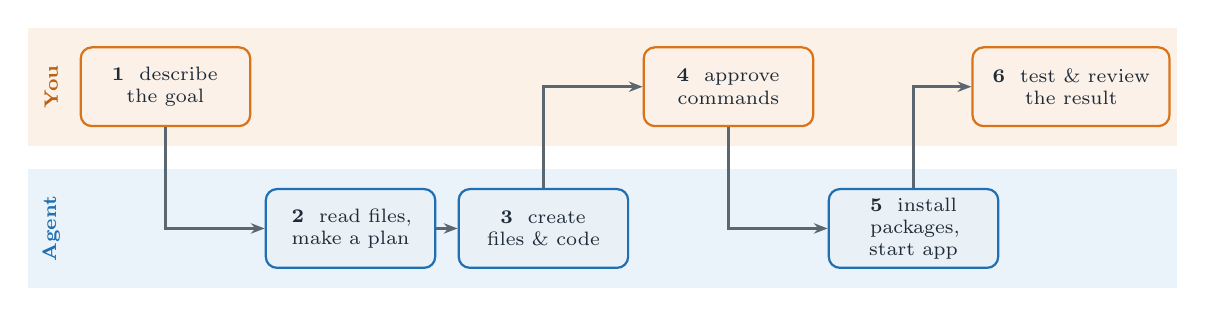
\begin{tikzpicture}[x=1cm,y=1cm,
      nd/.style={minimum width=2.1cm,minimum height=1.0cm,text width=1.8cm,inner ysep=3pt,font=\scriptsize,align=flush center}]
    % swim lanes (1.5 cm high: even the 3-line node keeps >= 4pt to the lane edge)
    \fill[cOrangeL!70] (0,0.65) rectangle (14.6,-0.85);
    \fill[cBlueL!70] (0,-1.15) rectangle (14.6,-2.65);
    \node[rotate=90,font=\scriptsize\bfseries,text=cOrange!85!black] at (0.3,-0.1) {You};
    \node[rotate=90,font=\scriptsize\bfseries,text=cBlue] at (0.3,-1.9) {Agent};
    % You lane
    \node[cbox=cOrange,nd] (a1) at (1.75,-0.1) {\textbf{1}\ \ describe\\the goal};
    \node[cbox=cOrange,nd] (a4) at (8.9,-0.1) {\textbf{4}\ \ approve\\commands};
    \node[cbox=cOrange,nd,minimum width=2.45cm,text width=2.15cm] (a6) at (13.25,-0.1) {\textbf{6}\ \ test \& review\\the result};
    % Agent lane
    \node[cbox=cBlue,nd] (b2) at (4.1,-1.9) {\textbf{2}\ \ read files,\\make a plan};
    \node[cbox=cBlue,nd] (b3) at (6.55,-1.9) {\textbf{3}\ \ create\\files \& code};
    \node[cbox=cBlue,nd] (b5) at (11.25,-1.9) {\textbf{5}\ \ install\\packages,\\start app};
    \draw[arr] (a1.south) |- (b2.west);
    \draw[arr] (b2) -- (b3);
    \draw[arr] (b3.north) |- (a4.west);
    \draw[arr] (a4.south) |- (b5.west);
    \draw[arr] (b5.north) |- (a6.west);
  \end{tikzpicture}
  \par\vspace{8pt}
  \begin{columns}[T,onlytextwidth]
    \begin{column}{0.48\textwidth}
      \begin{keybox}[The agent's tools]
        read and edit files \textbullet\ run terminal\\commands \textbullet\ read error messages\\and try again\strut
      \end{keybox}
    \end{column}
    \begin{column}{0.48\textwidth}
      \begin{warnbox}[Your job]
        a precise goal \textbullet\ conscious approvals \textbullet\\checking that the rules\\are \emph{really} implemented\strut
      \end{warnbox}
    \end{column}
  \end{columns}
  \note{Debrief the demo with this diagram. The orange boxes are the moments where a human decides; the blue boxes are the agent's work. The agent is not magic: it is a language model that can use tools -- reading and writing files and running terminal commands -- in a loop until the task looks done. The LLM deck explains this mechanism in detail.\par
  Now test the rules together: open the flagged table, find a hotel claim above 180 euros, check a Saturday date, search for a duplicate. Ask the students: ``How would you know if the duplicate rule is wrong?'' This is exactly the review habit we want.\par
  Mention that the agent asked before running commands because the permission level was set to Manual -- we will keep it that way in class.}
\end{frame}

% ------------------------------------------------------------------
\begin{frame}{Why this matters for AI-driven automation}
  \vspace{4pt}
  \begin{columns}[T,onlytextwidth]
    \begin{column}{0.315\textwidth}
      \begin{card}[cTeal]{\faFlask\ \ Test ideas cheaply}[equal height group=why]
        A clickable prototype in hours: learn early whether an automation idea is worth it.
      \end{card}
    \end{column}
    \begin{column}{0.315\textwidth}
      \begin{card}[cBlue]{\faExchange*\ \ The bottleneck shifts}[equal height group=why]
        From \emph{typing code} to \emph{specifying} and \emph{verifying} -- core business skills.
      \end{card}
    \end{column}
    \begin{column}{0.315\textwidth}
      \begin{card}[cPurple]{\faComments\ \ A shared language}[equal height group=why]
        A running prototype says more than twenty pages of requirements.
      \end{card}
    \end{column}
  \end{columns}
  \vspace{4pt}
  \begin{warnbox}[But: a prototype is not a product]
    Security, data protection, tests and operations still need professionals -- see the wrap-up.
  \end{warnbox}
  \takeaway{Business people who can prototype become better partners for IT --\\not replacements for it.}
  \note{Connect the demo to the module theme. Automation projects often fail not because of technology, but because requirements are vague and nobody tests the idea early. A prototype makes the idea concrete: users can click through it, disagree with it, and improve it.\par
  The second card is the key insight: when an agent can type the code, the scarce skills are precise specification and careful verification. Business students are well prepared for both -- they know the process and the rules.\par
  Balance the enthusiasm with the warning box. Ask: ``What would be missing before the finance department could use this app with real employee data?'' Collect answers such as access control, data protection, audit trail -- and keep them for the wrap-up.}
\end{frame}

% ------------------------------------------------------------------
\begin{frame}{``Vibe coding'' vs.\ AI-assisted coding}{Same tools, very different attitude}
  % badbox / keybox look, but with equal heights (tcolorbox equal height group)
  \begin{columns}[T,onlytextwidth]
    \begin{column}{0.485\textwidth}
      \begin{tcolorbox}[aidabase,colback=cRedL,borderline west={3pt}{0pt}{cRed},equal height group=d1aQuote]
        {\color{cRed}\bfseries\faQuoteLeft\ \ Vibe coding \muted{\normalfont(Karpathy, 2025)}}\par\vspace{1pt}
        {\footnotesize ``[\ldots] fully give in to the vibes, embrace exponentials, and forget that\\the code even exists.''\par}
      \end{tcolorbox}
    \end{column}
    \begin{column}{0.485\textwidth}
      \begin{tcolorbox}[aidabase,colback=cTealL,borderline west={3pt}{0pt}{cTeal},equal height group=d1aQuote]
        {\color{cTeal}\bfseries\faQuoteLeft\ \ AI-assisted coding \muted{\normalfont(Willison, 2025)}}\par\vspace{1pt}
        {\footnotesize ``[If you] reviewed it, tested it thoroughly and made sure you could explain how it works [\ldots] that's not vibe coding,\\it's software development.''\par}
      \end{tcolorbox}
    \end{column}
  \end{columns}
  \vspace{5pt}
  {\footnotesize
  \renewcommand{\arraystretch}{1.05}
  \begin{tabular}{@{}p{6.35cm} >{\centering\arraybackslash}p{3.1cm} >{\centering\arraybackslash}p{4.4cm}@{}}
    \toprule
    & \textbf{Vibe coding} & \textbf{AI-assisted coding}\\
    \midrule
    You read and understand the changes & \nomark & \yesmark\\
    You run and test it, including an error case & \nomark & \yesmark\\
    Every working step is committed to Git & \nomark & \yesmark\\
    \bottomrule
  \end{tabular}}
  \takeaway{Our rule: you own every line you run or share -- no matter who (or what) typed it.}
  \source{Karpathy (2025); Willison (2025)}
  \note{Andrej Karpathy coined the term ``vibe coding'' in a post on X on 2 February 2025. He himself wrote that it was ``not too bad for throwaway weekend projects''. The term spread quickly and is now often used for any AI-supported programming -- which is misleading.\par
  Simon Willison drew the line clearly in March 2025: if you review, test and can explain the code, it is not vibe coding, it is software development. That is why this course speaks of \textbf{AI-assisted coding}. The third row mentions Git: for now, a commit is simply a saved snapshot of the project you can return to -- Part 3 explains it properly.\par
  Ask the students which column they would want their bank's developers to be in. The point is not to forbid fast experimentation, but to know which mode you are in -- and to switch to the right-hand column as soon as real data or other people are involved.}
\end{frame}

% ------------------------------------------------------------------
\begin{frame}{What the evidence says}{AI assistance is powerful -- and uneven}
  \vspace{4pt}
  \begin{columns}[T,onlytextwidth]
    \begin{column}{0.315\textwidth}
      \begin{card}[cGreen]{\faArrowUp\ \ Well-defined tasks}[equal height group=ev]
        In controlled experiments, people with an AI assistant finish clearly specified tasks much faster.
        \par\vspace{3pt}\muted{\scriptsize Peng et al. (2023);\\Noy \& Zhang (2023)\par}
      \end{card}
    \end{column}
    \begin{column}{0.315\textwidth}
      \begin{card}[cOrange]{\faArrowDown\ \ Large, familiar code}[equal height group=ev]
        Experienced developers working in their own large projects were \emph{slower} with AI tools -- while believing they were faster.
        \par\vspace{3pt}\muted{\scriptsize Becker et al. (2025)}
      \end{card}
    \end{column}
    \begin{column}{0.315\textwidth}
      \begin{card}[cPurple]{\faChartLine\ \ The jagged frontier}[equal height group=ev]
        Inside the AI's capability frontier, quality rises; just outside it, people who rely on AI make more mistakes.
        \par\vspace{3pt}\muted{\scriptsize Dell'Acqua et al. (2026)}
      \end{card}
    \end{column}
  \end{columns}
  \takeaway{Using AI well is a skill: know when to delegate, when to check --\\and when to think for yourself.}
  % sources are cited in the cards (the footer line would run into the section label)
  \note{Exact figures for questions: Peng et al. (2023): 95 professional developers wrote an HTTP server in JavaScript; the group with GitHub Copilot finished 55.8\% faster (95\% CI 21--89\%). Noy \& Zhang (2023, Science): 453 professionals, writing tasks with ChatGPT: 40\% less time, 18\% higher quality.\par
  Becker et al. (2025, METR): 16 experienced open-source developers, 246 tasks in their own repositories. They expected AI to save 24\% of the time and afterwards believed it had saved 20\% -- in fact they took 19\% longer.\par
  Dell'Acqua et al. (2026, Organization Science): 758 BCG consultants with GPT-4. Inside the frontier: 12.2\% more tasks, 25.1\% faster, about 32\% higher quality. On a task outside the frontier, AI users were 19 percentage points less likely to be correct.\par
  Update (METR blog, 24 Feb 2026; follow-up with 57 developers and 800+ tasks from late 2025): point estimates of 18\% (returning) and 4\% (new developers) \emph{less} time with AI, but both confidence intervals include zero and METR calls the evidence very weak because of selection effects. Message: our POCs are well-defined tasks -- ideal for AI assistance. But always verify.}
\end{frame}

% ------------------------------------------------------------------
\begin{frame}{The AI-assisted coding loop}{Seconds to minutes per iteration -- with a commit whenever something works}
  \centering
  \begin{tikzpicture}[x=1cm,y=1cm]
    \foreach \a/\c/\n/\t in {90/cBlue/1/{Describe\\the goal},18/cTeal/2/{Agent\\generates},-54/cOrange/3/{Review\\the changes},-126/cPurple/4/{Run \& test},162/cGreen/5/{Refine the\\description}}
      {\node[cbox=\c,minimum width=2.45cm,minimum height=0.95cm,text width=2.25cm,font=\footnotesize,align=flush center] (n\n) at ({3.4*cos(\a)},{1.85*sin(\a)}) {\textbf{\n}\ \ \t};}
    \draw[arr,line width=1.1pt] (n1) to[bend left=18] (n2);
    \draw[arr,line width=1.1pt] (n2) to[bend left=18] (n3);
    \draw[arr,line width=1.1pt] (n3) to[bend left=18] (n4);
    \draw[arr,line width=1.1pt] (n4) to[bend left=18] (n5);
    \draw[arr,line width=1.1pt] (n5) to[bend left=18] (n1);
    \node[sbox=cNavy,circle,minimum size=1.55cm,text width=1.35cm,font=\scriptsize,align=flush center] at (0,0) {\faCodeBranch\\commit when it works};
  \end{tikzpicture}
  \vspace{-4pt}
  \takeaway{Small steps win: one feature per loop, test it, commit it -- then the next one.}
  \note{This loop replaces the classic ``read documentation, learn syntax, write, debug, search the web'' cycle. The big difference is speed: one iteration takes seconds to minutes instead of hours.\par
  Stress steps 3 and 4 -- they are where learning and quality happen. Reviewing means reading the diff the agent produced and asking it to explain anything unclear. Testing means running the app and trying at least one normal case and one error case.\par
  The commit in the centre is the safety net: whenever the app works, commit. If the next iteration breaks something, you can always go back. Students who skip commits usually lose work in the first POC -- say this explicitly.}
\end{frame}

% ------------------------------------------------------------------
\begin{frame}{From autocomplete to agents}{Five years of GitHub Copilot}
  \vspace{6pt}
  \centering
  
\begin{tikzpicture}[x=1cm,y=1cm]
    \draw[line width=1.6pt,cLine] (0,0) -- (14.5,0);
    \foreach \x/\c/\d/\t in {0.9/cGray/{Jun 2021}/{technical\\preview},3.9/cGray/{Jun 2022}/{generally\\available},6.9/cBlue/{Dec 2023}/{Copilot Chat\\generally available},9.9/cTeal/{Feb--Apr 2025}/{agent mode\\in VS Code},12.9/cPurple/{Sep 2025}/{cloud coding agent\\generally available}}
      {\fill[\c] (\x,0) circle (4pt);
       \node[font=\scriptsize\bfseries,text=\c,anchor=base,inner sep=0pt] at (\x,0.3) {\d};
       \node[font=\scriptsize,text=cInk,below=6pt,align=center] at (\x,0) {\t};}
  \end{tikzpicture}
  \par\vspace{16pt}
  \begin{columns}[T,onlytextwidth]
    \begin{column}{0.315\textwidth}
      \begin{card}[cGray]{Gen.\,1: autocomplete}[equal height group=gen]
        AI completes the line or function you are typing.
      \end{card}
    \end{column}
    \begin{column}{0.315\textwidth}
      \begin{card}[cBlue]{Gen.\,2: chat}[equal height group=gen]
        AI answers questions, explains and rewrites code blocks.
      \end{card}
    \end{column}
    \begin{column}{0.315\textwidth}
      \begin{card}[cTeal]{Gen.\,3: agents}[equal height group=gen]
        AI plans, edits many files, runs commands and iterates -- \emph{with your approval}.
      \end{card}
    \end{column}
  \end{columns}
  \note{Dates, all from GitHub's own announcements: technical preview 29 June 2021; general availability 21 June 2022 (free for verified students from the start); Copilot Chat generally available 29 December 2023; agent mode preview in VS Code Insiders 6 February 2025 and available to all VS Code users in April 2025 (VS Code 1.99); the Copilot coding agent, which works on GitHub issues in the cloud and opens pull requests, became generally available on 25 September 2025 (now called ``Copilot cloud agent'').\par
  The point for students: within four years the tool went from suggesting a line to autonomously changing a whole project. That is why the human role moves from typing to specifying and reviewing. In this course we use generation 3 -- the agent in VS Code -- but keep generations 1 and 2 in mind: they are still useful for small edits and questions.}
\end{frame}

% ------------------------------------------------------------------
\begin{frame}{What is a proof of concept (POC)?}{And what it deliberately leaves out}
  \vspace{2pt}
  \begin{columns}[T,onlytextwidth]
    \begin{column}{0.55\textwidth}
      \begin{keybox}[Proof of concept]
        \begin{itemize}\setlength{\itemsep}{2pt}
          \item a \textbf{running prototype} that proves\\one concrete idea
          \item small and focused -- built in hours to days
          \item optimised for \textbf{learning speed},\\not robustness
          \item just enough to answer\\one question -- no more
        \end{itemize}
      \end{keybox}
    \end{column}
    \begin{column}{0.42\textwidth}
      \begin{warnbox}[Deliberately left out]
                tests, authentication, multiple users, caching, background jobs, deployment, visual polish
      \end{warnbox}
      \vskip3pt % gap between stacked boxes: 6pt
      \begin{infobox}[Typical POC questions]
        Can we detect this automatically? Is the data good enough? Would users accept this workflow?
      \end{infobox}
    \end{column}
  \end{columns}
  \takeaway{Rule of thumb: better to prove three things quickly than to perfect one thing slowly.}
  \note{Define the term precisely, because students will hear ``POC'', ``prototype'' and ``MVP'' used interchangeably in companies. A POC answers a question -- technical feasibility, data quality, user acceptance. An MVP (minimum viable product) is already something real users use in production.\par
  The warning box lists what we skip on purpose. This is not sloppiness: leaving these things out is what makes a POC fast. The danger in practice is when a POC is silently promoted to production without adding them.\par
  Ask for an example from the expense-claim demo: which question did it answer? (Answer: can the three policy rules be checked automatically on our claim data?)}
\end{frame}

% ------------------------------------------------------------------
\begin{frame}{What we will build}{Three POCs -- each one adds architecture, nothing is taken away}
  \vspace{4pt}
  \begin{columns}[T,onlytextwidth]
    \begin{column}{0.315\textwidth}
      \begin{card}[cBlue]{POC 1 \textbullet\ Data app}[equal height group=poc]
        \textbf{Streamlit} only\par\vspace{2pt}
        upload a CSV, descriptive statistics, charts\par\vspace{4pt}
        \muted{\scriptsize one process, one file}
      \end{card}
    \end{column}
    \begin{column}{0.315\textwidth}
      \begin{card}[cTeal]{POC 2 \textbullet\ Three tiers}[equal height group=poc]
        Streamlit + \textbf{FastAPI}\\+ \textbf{SQLite}\par\vspace{2pt}
        same use case, professional structure\par\vspace{4pt}
        \muted{\scriptsize two processes, a REST API, a~database}
      \end{card}
    \end{column}
    \begin{column}{0.315\textwidth}
      \begin{card}[cPurple]{POC 3 \textbullet\ ML app}[equal height group=poc]
        + an \textbf{XGBoost} model\par\vspace{2pt}
        predict customer churn, log every prediction\par\vspace{4pt}
        \muted{\scriptsize data $\rightarrow$ model $\rightarrow$ API $\rightarrow$ UI}
      \end{card}
    \end{column}
  \end{columns}
  \par\vspace{8pt}
  \centering
  
\begin{tikzpicture}[x=1cm,y=1cm]
    \node[cbox=cBlue,font=\scriptsize,minimum width=2.1cm] (s) at (0,0) {\faDesktop\ Streamlit};
    \node[cbox=cTeal,font=\scriptsize,minimum width=2.1cm] (f) at (3.4,0) {\faServer\ FastAPI};
    \node[cbox=cOrange,font=\scriptsize,minimum width=2.1cm] (d) at (6.8,0) {\faDatabase\ SQLite};
    \node[cbox=cPurple,font=\scriptsize,minimum width=2.1cm] (m) at (10.2,0) {\faBrain\ XGBoost};
    \draw[arr] (s) -- (f); \draw[arr] (f) -- (d); \draw[arr] (d) -- (m);
    \node[font=\scriptsize,text=cGray,below=2pt] at (s.south) {POC 1};
    \node[font=\scriptsize,text=cGray,below=2pt] at ($(f.south)!0.5!(d.south)$) {+ POC 2};
    \node[font=\scriptsize,text=cGray,below=2pt] at (m.south) {+ POC 3};
  \end{tikzpicture}
  \note{Give the big picture before the setup, so students know why they install each tool. POC 1 is a single Streamlit app -- the fastest way to a useful data tool. POC 2 solves exactly the same problem, but with a professional architecture: a separate backend (FastAPI) and a database (SQLite). Comparing POC 1 and POC 2 shows what architecture really means. POC 3 adds a machine-learning model and turns the app into a small ML product.\par
  Each POC builds on the previous one, and nothing is taken away. By the end, students have seen all typical building blocks of a data-driven business application.\par
  Transition: ``To build these, you need a toolchain. Let's set it up -- now, together.''}
\end{frame}
% ==================================================================
% PART 2 -- SETUP
% ==================================================================
\section{Setting up your toolchain}
\partframe{Session 1}{Seven steps, in this order -- we do them together in class.}{%
  \darkitem{Create a GitHub account and apply for GitHub Education}
  \darkitem{Install Git, Python 3.13 and VS Code}
  \darkitem{Sign in to Copilot and run a first test}
  \darkitem{Know the chat controls that keep you in charge}}

% ------------------------------------------------------------------
\begin{frame}{Your toolchain at a glance}{Five tools, one job each}
  \centering
  % flush center: no stretched word spaces; same minimum height for all five nodes
  \begin{tikzpicture}[x=1cm,y=1cm]
    \node[comp=cNavy,minimum width=2.45cm,text width=2.25cm,minimum height=2.0cm,align=flush center] (gh) at (0,0) {\faGithub\\[2pt]\textbf{GitHub}\\\scriptsize account, repos,\\Copilot licence};
    \node[comp=cTeal,minimum width=2.45cm,text width=2.25cm,minimum height=2.0cm,align=flush center] (cp) at (3.85,0) {\faRobot\\[2pt]\textbf{Copilot}\\\scriptsize AI assistant \&\\agent};
    \node[comp=cBlue,minimum width=2.45cm,text width=2.25cm,minimum height=2.0cm,align=flush center] (vs) at (7.7,0) {\faCode\\[2pt]\textbf{VS Code}\\\scriptsize editor, terminal,\\chat};
    \node[comp=cOrange,minimum width=2.45cm,text width=2.25cm,minimum height=2.0cm,align=flush center] (py) at (11.55,0) {\faPython\\[2pt]\textbf{Python 3.13}\\\scriptsize runs your code\\\mbox{}};
    \node[comp=cPurple,minimum width=2.45cm,text width=2.25cm,minimum height=2.0cm,align=flush center] (git) at (5.8,-2.4) {\faCodeBranch\\[2pt]\textbf{Git}\\\scriptsize version control\\on your laptop};
    \draw[arr] (gh) -- node[lbl,above]{licence} (cp);
    \draw[arr] (cp) -- node[lbl,above]{built in} (vs);
    \draw[arr] (vs) -- node[lbl,above]{runs} (py);
    \draw[darr] (git.west) -| node[lbl,pos=0.75,left=2pt]{push / pull} (gh.south);
    \draw[darr] (git.east) -| node[lbl,pos=0.75,right=2pt]{used by} (vs.south);
  \end{tikzpicture}
  \takeaway{GitHub stores your code and your licence; VS Code is where you work;\\Git keeps every version.}
  \note{Give the mental model before installing anything. GitHub is a website: it hosts repositories (project folders with history) and manages the Copilot licence. Copilot is the AI -- in VS Code it is built in, you only need to sign in. VS Code is the editor where you write, run and chat. Python is the language our prototypes use. Git is a program on your laptop that records versions; VS Code uses it, and it synchronises with GitHub.\par
  Common confusion to address: ``Git'' and ``GitHub'' are not the same. Git is the tool, GitHub is a service built around it -- like email and Gmail.\par
  Timing: in a 90-minute Session 1 the front slides and Part 1 take about 35 minutes, so about 55 remain for the setup. That works if students did steps 1 and 2 before class (next slide): steps 3--7 take about 30--40 minutes plus troubleshooting, and whatever is unfinished becomes homework (``Setup done?'').}
\end{frame}

% ------------------------------------------------------------------
\begin{frame}{Before class: start today}{Verification takes days, not minutes}
  \vspace{2pt}
  \begin{columns}[T]
    \begin{column}{0.48\textwidth}
      \begin{card}[cNavy]{\numdot{1}\ \ Create a GitHub account}[equal height group=before]
        \href{https://github.com/signup}{\texttt{github.com/signup}} -- ideally with your HSBI email address; switch on two-factor authentication.
      \end{card}
    \end{column}
    \begin{column}{0.48\textwidth}
      \begin{card}[cTeal]{\numdot[cNavy]{2}\ \ Apply for GitHub Education}[equal height group=before]
        Verification usually takes a few days -- longer at the start of the semester. Apply as soon as your account exists.
      \end{card}
    \end{column}
  \end{columns}
  \vspace{6pt}
  \begin{warnbox}[No approval yet? No problem.]
    Every account can use \textbf{Copilot Free} at once. After approval, activate Copilot Student yourself (Education benefits $\rightarrow$ \emph{Learn more}) -- never pay.
  \end{warnbox}
  \takeaway{Do both today -- verification takes days, and Copilot Free bridges the gap.}
  \note{This slide is meant to be sent out in advance (email or learning platform). The student verification by GitHub is the only step in the setup that students cannot speed up: GitHub's docs state that approval and Copilot activation are separate steps and that the student benefit ``can take several days to finish applying after verification''; eligibility is re-evaluated every month (as of Sep 2026).\par
  Background: in spring 2026 GitHub paused new sign-ups for individual Copilot plans for some weeks and reopened them gradually from June 2026 -- another reason to apply early.\par
  Reassure students that nobody is blocked: Copilot Free works immediately after signing in and is sufficient to follow the first session. Important (GitHub docs ``Access GitHub Copilot for free as a student''): after approval, students open their Education benefits, click \emph{Learn more} under the free developer resources and follow the prompts; while the benefit is still being applied, the Copilot settings page is the documented fallback. If only paid options appear, they should not buy anything but wait or ask.}
\end{frame}

% ------------------------------------------------------------------
\begin{frame}{Seven steps -- in this order}{Later steps depend on earlier ones}
  \vspace{2pt}
  \begin{columns}[T]
    \begin{column}{0.54\textwidth}
      {\small
      \renewcommand{\arraystretch}{1.42}
      \begin{tabular}{@{}c l r@{}}
        \toprule
        & \textbf{Step} & \textbf{Time}\\
        \midrule
        \numdot{1} & GitHub account (with 2FA) & 5 min\\
        \numdot{2} & Apply for GitHub Education & 10 min\\
        \numdot{3} & Install Git & 5--10 min\\
        \numdot{4} & Install Python 3.13 & 5--10 min\\
        \numdot{5} & Install VS Code + Python ext. & 5 min\\
        \numdot{6} & Sign in to Copilot in VS Code & 2 min\\
        \numdot{7} & First test with Copilot & 10 min\\
        \bottomrule
      \end{tabular}}
    \end{column}
    \begin{column}{0.40\textwidth}
      \begin{keybox}[Definition of done]
        You can run a Python script in VS Code \emph{and} Copilot answers a question in the chat.
      \end{keybox}
      \vskip3pt % gap between stacked boxes: 6pt
      \begin{infobox}[Work in pairs]
        One person installs, the other reads the next step aloud -- then swap. Problems are solved twice as fast.
      \end{infobox}
    \end{column}
  \end{columns}
  \note{Show the full sequence before starting so students can pace themselves. The times are rough estimates for a laptop with a decent connection; downloads in a full lecture hall can be slower -- consider asking students to download the installers beforehand.\par
  The order matters: Git should be installed before VS Code so that VS Code finds it immediately; Python before the first test; the GitHub account before signing in to Copilot.\par
  Walk around the room during this part. The most frequent problems are listed on the troubleshooting slide at the end of this part -- keep it open on a second screen.}
\end{frame}

% ------------------------------------------------------------------
\begin{frame}{\stepbadge{1}\ \ Create your GitHub account}
  \vspace{2pt}
  \begin{columns}[T]
    \begin{column}{0.55\textwidth}
      \begin{enumerate}\setlength{\itemsep}{4pt}
        \item Go to \href{https://github.com/signup}{\texttt{github.com/signup}}
        \item Register with your \textbf{HSBI email address} (you can add a private address later)
        \item Choose a \textbf{professional username} -- it will appear in your CV and portfolio
        \item Confirm your email address
        \item Enable \textbf{two-factor authentication} \mbox{(Settings $\rightarrow$ Password and authentication)}
      \end{enumerate}
    \end{column}
    \begin{column}{0.41\textwidth}
      \begin{keybox}[Good usernames]
        \texttt{cweisser}, \texttt{christoph-weisser}\\
        \muted{not:} \texttt{xX\_coder99\_Xx}
      \end{keybox}
      \vskip3pt % gap between stacked boxes: 6pt
      \begin{infobox}[Why 2FA now?]
        GitHub Education requires it --\\and it protects your code\\and your licence.
      \end{infobox}
    \end{column}
  \end{columns}
  \takeaway{Your GitHub profile is part of your professional identity -- treat it like LinkedIn.}
  \note{Most students will need about five minutes. Encourage a neutral, professional username: recruiters in data and IT roles do look at GitHub profiles, and the POCs of this course are a nice first portfolio.\par
  Two-factor authentication: GitHub's student-benefit application requires 2FA to be enabled (as of Sep 2026). An authenticator app (e.g. Microsoft Authenticator, Google Authenticator) is the easiest option; students should also store the recovery codes safely.\par
  If a student already has a GitHub account with a private email address, they can simply add the HSBI address under Settings $\rightarrow$ Emails -- no second account needed.}
\end{frame}

% ------------------------------------------------------------------
\begin{frame}{\stepbadge{2}\ \ Apply for GitHub Education}{Verified students get the \textbf{GitHub Copilot Student} plan}
  \vspace{2pt}
  \begin{columns}[T]
    \begin{column}{0.50\textwidth}
      {\small\bfseries\color{cNavy}How to apply}\par\vspace{3pt}
      \begin{enumerate}\setlength{\itemsep}{5pt}\small
        \item Open\\{\footnotesize\href{https://github.com/settings/education/benefits}{\texttt{github.com/settings/education/benefits}}}
        \item \emph{Start an application}, select HSBI
        \item Upload \textbf{proof of enrolment} (dated)
        \item Allow \textbf{location + camera}; \textbf{no VPN}
      \end{enumerate}
    \end{column}
    \begin{column}{0.46\textwidth}
      \begin{keybox}[What you get (as of Sep 2026)]
        unlimited code completions \textbullet\ monthly allowance of AI credits for chat and agent \textbullet\ automatic model selection
      \end{keybox}
      \vskip3pt % gap between stacked boxes: 6pt
      \begin{warnbox}[Common rejections]
        blurry or undated document \textbullet\ name differs from your GitHub billing info \textbullet\ VPN switched on
      \end{warnbox}
    \end{column}
  \end{columns}
  \takeaway{Until approval arrives, simply use Copilot Free.}
  \note{As of Sep 2026 (plans change -- check the docs): since March 2026 verified students get \textbf{GitHub Copilot Student} instead of Copilot Pro -- agent mode, 200 AI credits per month (from 1 June 2026, replacing ``premium requests'') and automatic model choice (``Auto'').\par
  Requirements in GitHub's docs: currently enrolled, dated proof of enrolment and, if your school's applicants usually verify that way, an academic email address. The verification flow additionally checks location and camera access, no VPN, two-factor authentication, and that the full name in your GitHub billing information matches the document.\par
  Credits are token-based and reset on the 1st of each month without carry-over; agent sessions use them fastest. When they run out, chat and agent pause until the next month (unless someone sets a paid budget -- don't); code completions stay unlimited. Usage is shown via the Copilot icon in the Status Bar. Sources: docs.github.com (Copilot plans; usage-based billing for individuals), GitHub's Community announcement on Copilot for Students (the 200 credits) and the GitHub changelog of 13 March 2026.}
\end{frame}

% ------------------------------------------------------------------
\begin{frame}[fragile]{\stepbadge{3}\ \ Install Git}{The version-control program on your laptop}
  \vspace{2pt}
  \begin{columns}[T]
    \begin{column}{0.57\textwidth}
      \begin{card}[cBlue]{\faWindows\ \ Windows}[equal height group=git]
        Installer from \href{https://git-scm.com}{\texttt{git-scm.com}} (default options), or in a terminal:
\begin{lstlisting}[language=bash]
winget install --id Git.Git -e --source winget
\end{lstlisting}
      \end{card}
    \end{column}
    \begin{column}{0.39\textwidth}
      \begin{card}[cGray]{\faApple\ \ macOS}[equal height group=git]
        Apple's Command Line Tools include Git:
\begin{lstlisting}[language=bash]
xcode-select --install
\end{lstlisting}
      \end{card}
    \end{column}
  \end{columns}
  \vspace{12pt}
  {\small\bfseries\color{cNavy}Then, in a new terminal (PowerShell / Terminal): check and introduce yourself}
\begin{lstlisting}[language=bash]
git --version                                   # e.g. git version 2.5x
git config --global user.name  "Firstname Lastname"
git config --global user.email "you@hsbi.de"    # same address as on GitHub
\end{lstlisting}
  \note{Git must be installed separately -- VS Code has Git support built in, but it needs the Git program itself. On Windows, both the official installer from git-scm.com and winget work; the installer's default options are fine. On macOS, \texttt{xcode-select --install} installs Apple's Command Line Tools, including Git; users of Homebrew can alternatively run \texttt{brew install git}.\par
  The two \texttt{git config} lines tell Git who you are; every commit is labelled with this name and email. Use the same email address as on GitHub so that commits are linked to the profile.\par
  Many students have never opened a terminal: on Windows search for \emph{PowerShell} in the Start menu, on macOS open \emph{Terminal} via Spotlight; from Step 7 on we use the terminal built into VS Code. Tip: close and reopen the terminal (and VS Code) after installing, otherwise the \texttt{git} command may not be found yet.}
\end{frame}

% ------------------------------------------------------------------
\begin{frame}[fragile]{\stepbadge{4}\ \ Install Python 3.13}{Not the newest version -- the one all our packages support}
  \vspace{2pt}
  \begin{columns}[T]
    \begin{column}{0.49\textwidth}
      \begin{card}[cBlue]{\faWindows\ \ Windows}[equal height group=d1aPy]
        From \href{https://www.python.org/downloads/}{\texttt{python.org/downloads}}: the \emph{Python install manager}, then:
\begin{lstlisting}[language=bash]
py install 3.13
\end{lstlisting}
        \muted{\scriptsize Classic installer: tick ``Add python.exe to PATH''.}
      \end{card}
    \end{column}
    \begin{column}{0.47\textwidth}
      \begin{card}[cGray]{\faApple\ \ macOS}[equal height group=d1aPy]
        Download the macOS installer for \textbf{Python 3.13.x} from \href{https://www.python.org/downloads/}{\texttt{python.org/downloads}} and run it.\par\vspace{2pt}
        \muted{\scriptsize On macOS the command is usually \texttt{python3}.}
      \end{card}
    \end{column}
  \end{columns}
  \vspace{12pt}
  \begin{columns}[T]
    \begin{column}{0.49\textwidth}
{\small\bfseries\color{cNavy}Check in a new terminal}
\begin{lstlisting}[language=bash]
python --version   # macOS: python3 --version
Python 3.13.x
\end{lstlisting}
    \end{column}
    \begin{column}{0.47\textwidth}
      \begin{warnbox}[Why not 3.14 or 3.15?]
        Brand-new versions such as 3.15 often lack ready-made packages (e.g.\ PyTorch). Python 3.13 works with everything we use.
      \end{warnbox}
    \end{column}
  \end{columns}
  \note{As of early October 2026 the newest stable release is Python 3.14 (3.14.8, 30 September 2026); 3.15.0 has slipped to 9 October 2026. We deliberately use 3.13: it is still supported (security fixes until October 2029; 3.13.16 of 30 September 2026 is the last 3.13 release with Windows/macOS installers), and all our packages -- including xgboost, numpy, faiss-cpu, chromadb and PyTorch (needed by sentence-transformers in the LLM deck) -- provide ready-made wheels for it. For 3.15, PyTorch and onnxruntime had no wheels yet.\par
  Windows: python.org recommends the new \emph{Python install manager} (\texttt{py install}, \texttt{python}); the classic installer has been deprecated since 3.14 but is still available -- if used, tick ``Add python.exe to PATH''.\par
  Careful on Windows: with the install manager, plain \texttt{python} starts the \emph{newest} installed version (and installs the latest one if none exists -- that will be 3.15 once it is released). So create environments explicitly with \texttt{py -V:3.13 -m venv .venv} (Python docs, ``Using Python on Windows''). Check with \texttt{py list}. Inside an activated venv, \texttt{python} is always the right version.}
\end{frame}

% ------------------------------------------------------------------
\begin{frame}{\stepbadge{5}\ \ Install VS Code and the Python extension}
  \vspace{2pt}
  \begin{columns}[T]
    \begin{column}{0.53\textwidth}
      \begin{enumerate}\setlength{\itemsep}{4pt}
        \item Download from \href{https://code.visualstudio.com}{\texttt{code.visualstudio.com}} and install with the default options
        \item Open the \textbf{Extensions} view \mbox{(\kbd{Ctrl+Shift+X}\,/\,\kbd{Cmd+Shift+X})}
        \item Install \textbf{Python} by Microsoft (brings Pylance and the debugger)
        \item Optional: \textbf{Jupyter} by Microsoft
      \end{enumerate}
    \end{column}
    \begin{column}{0.43\textwidth}
      \begin{keybox}[Good news]
        GitHub Copilot is \textbf{built into VS Code}: there is no separate Copilot extension to install any more.
      \end{keybox}
      \vskip3pt % gap between stacked boxes: 6pt
      \begin{infobox}[Windows]
        Keep the option ``Add to PATH'' ticked -- then you can open any folder with \mbox{\texttt{code .}}
      \end{infobox}
    \end{column}
  \end{columns}
  \takeaway{VS Code is your cockpit: files on the left, code in the middle,\\terminal below, chat on the right.}
  \note{VS Code is free and available for Windows, macOS and Linux. The Python extension from Microsoft adds syntax highlighting, code completion via Pylance, running and debugging, and the selection of virtual environments.\par
  Copilot: since early 2026 the former ``GitHub Copilot'' extension has been deprecated, and all AI features run through the built-in, open-source Copilot Chat integration of VS Code. Students therefore only need to sign in (next step). Older tutorials that tell you to install two Copilot extensions are outdated.\par
  VS Code now ships updates weekly (as of Sep 2026), so menus and labels change often -- if a student's screen looks slightly different from yours, that is normal.}
\end{frame}

% ------------------------------------------------------------------
\begin{frame}{\stepbadge{6}\ \ Sign in to GitHub Copilot}
  \vspace{2pt}
  \begin{columns}[T]
    \begin{column}{0.53\textwidth}
      \begin{enumerate}\setlength{\itemsep}{4pt}
        \item Hover over the \textbf{Copilot icon} in the \mbox{Status Bar} (bottom right)
        \item Choose \textbf{Use AI Features}
        \item Sign in with your \textbf{GitHub account} in the browser and allow VS Code
        \item Back in VS Code: open the chat with \mbox{\kbd{Ctrl+Alt+I}\,/\,\kbd{Ctrl+Cmd+I}}
      \end{enumerate}
    \end{column}
    \begin{column}{0.43\textwidth}
      \begin{keybox}[Check your plan]
        On github.com: profile picture $\rightarrow$ \emph{Copilot settings} shows whether you are on \emph{Student} or \emph{Free}.
      \end{keybox}
      \vskip3pt % gap between stacked boxes: 6pt
      \begin{warnbox}[Privacy]
        Don't paste personal or confidential company data into the chat.
      \end{warnbox}
    \end{column}
  \end{columns}
  \takeaway{No subscription yet? Signing in enrols you in Copilot Free automatically.}
  \note{The sign-in path as of September 2026 (VS Code docs ``Set up GitHub Copilot''): hover over the Copilot icon in the Status Bar, choose ``Use AI Features'', pick the sign-in method and authenticate in the browser. Alternatives: the Accounts menu or the command ``GitHub Copilot: Sign in''. Accounts without a paid or student plan are signed up for Copilot Free.\par
  Mention data protection: prompts and code snippets are sent to GitHub's service for processing. For our synthetic demo data this is unproblematic; for real customer or employee data it would require a company agreement. VS Code also states that telemetry is enabled in the free version and can be switched off in the settings.\par
  If the Copilot icon is missing, check that AI features have not been disabled in the settings.}
\end{frame}

% ------------------------------------------------------------------
\begin{frame}[fragile]{\stepbadge{7}\ \ First test: environment, script, Copilot}
  \vspace{2pt}
  \begin{columns}[T,onlytextwidth]
    \begin{column}{0.45\textwidth}
{\small\bfseries\color{cNavy}Create a folder \file{hello-poc},\\open it via \mbox{\emph{File $\rightarrow$ Open Folder}},\\then \mbox{\emph{Terminal $\rightarrow$ New Terminal}}:}
\begin{lstlisting}[language=bash]
python3.13 -m venv .venv       # macOS
source .venv/bin/activate      # macOS
py -V:3.13 -m venv .venv       # Windows
.venv\Scripts\Activate.ps1     # Windows
\end{lstlisting}
{\small\bfseries\color{cNavy}Create \file{hello.py} and run it}
\begin{lstlisting}[language=Python]
print("Hello -- my setup works!")
\end{lstlisting}
\begin{lstlisting}[language=bash]
python hello.py
\end{lstlisting}
    \end{column}
        \begin{column}{0.52\textwidth}
      \begin{keybox}[Now try Copilot]
        \textbf{Inline:} type\\
        {\setlength{\fboxsep}{1.5pt}\colorbox{white}{\scriptsize\ttfamily\# function that returns the VAT for a net price}}\\
        and press \kbd{Enter} -- accept the grey suggestion with \kbd{Tab}.\par\vspace{3pt}
        \textbf{Chat (Ask):} ``Explain \texttt{hello.py} and what a virtual environment is.''
      \end{keybox}
      \vskip3pt % gap between stacked boxes: 6pt
      \begin{infobox}
        VS Code asks which Python to use? Pick the one inside \file{.venv}.
      \end{infobox}
    \end{column}
  \end{columns}
  \note{This is the definition-of-done test. Walk through it slowly on the projector. The virtual environment (\texttt{.venv}) is a project-specific Python installation -- Part 3 explains the concept; for now it is enough that each project gets its own.\par
  Windows PowerShell may refuse to run the activation script (``running scripts is disabled''). Fix, once per user: \texttt{Set-ExecutionPolicy -ExecutionPolicy RemoteSigned -Scope CurrentUser}. Alternatively use \texttt{.venv\textbackslash Scripts\textbackslash activate.bat} in cmd. We avoid \texttt{\&\&} chains because Windows PowerShell 5.1 does not support them, and we open folders via the menu because the \texttt{code} command needs extra setup on macOS.\par
  Let students try both: an inline suggestion (generation 1) and a chat question in Ask (generation 2). Ask is offered in the Local session target; in the Copilot target students write ``Only explain -- do not change any files'' in front of the question (see the next slides). Say where to create \texttt{hello-poc} (e.g.\ in Documents) -- it is the first question in every room. Congratulate everyone who gets here -- the rest of the course builds on it.}
\end{frame}

% ------------------------------------------------------------------
\begin{frame}{The chat view at a glance}{Four controls below the input box decide how the agent works}
  \centering
  \begin{tikzpicture}[x=1cm,y=1cm]
    % mock chat panel
    \draw[cLine,fill=cGrayL,rounded corners=4pt,line width=0.8pt] (0,0) rectangle (14.4,-2.35);
    \node[draw=cLine,fill=white,rounded corners=3pt,minimum width=13.8cm,minimum height=0.8cm,anchor=north west,align=left,text width=13.4cm,font=\footnotesize,text=cGray] at (0.3,-0.25)
      {Describe what you want to build \ldots};
    \node[pick,anchor=west] (p1) at (0.3,-1.65) {\faLaptop\ \ Session target: \textbf{Copilot}\ \faAngleDown};
    \node[pick,right=8.8pt of p1] (p2) {\faRobot\ \ Agent: \textbf{Agent}\ \faAngleDown};
    \node[pick,right=8.8pt of p2] (p3) {\faBrain\ \ Model: \textbf{Auto}\ \faAngleDown};
    \node[pick,right=8.8pt of p3] (p4) {\faShield*\ \ \textbf{Manual permissions}\ \faAngleDown};
        % explanations (left-aligned with their control; pills evenly spaced)
    \node[font={\scriptsize\hyphenpenalty=10000},text width=3.8cm,align=flush left,anchor=north west] at (p1.west |- 0,-2.65) {\textbf{Where it runs.}\\Start with \emph{Copilot}.};
    \node[font={\scriptsize\hyphenpenalty=10000},text width=2.6cm,align=flush left,anchor=north west] at (p2.west |- 0,-2.65) {\textbf{Which mode.}\\\emph{Agent} or \emph{Plan} (\texttt{/plan}).};
    \node[font={\scriptsize\hyphenpenalty=10000},text width=2.5cm,align=flush left,anchor=north west] at (p3.west |- 0,-2.65) {\textbf{Which LLM.}\\\emph{Auto} for students.};
    \node[font={\scriptsize\hyphenpenalty=10000},text width=3.6cm,align=flush left,anchor=north west] at (p4.west |- 0,-2.65) {\textbf{What needs your OK.}\\Always \emph{Manual} in class.};
  \end{tikzpicture}
  \takeaway{Beginner settings: Copilot \textbullet\ Agent (or Plan) \textbullet\ Auto \textbullet\ Manual permissions.}
  \note{This is a simplified mock-up of the chat input as of September 2026 (VS Code docs ``Agent harnesses'' and ``Approvals''). The four pickers: \textbf{Session target} -- which harness runs the session and where its tools operate; the docs recommend starting with \emph{Copilot}. \textbf{Agent} -- the mode with its instructions and tools: in Copilot sessions the default mode (the docs call it \emph{Agent} or \emph{Interactive}), \emph{Plan} (\texttt{/plan} switches to it) and \emph{Autopilot} (not in class) -- Copilot sessions offer no Ask; only the Local target lists Ask, Plan and Agent (plus custom agents). \textbf{Model} -- which LLM; on the Free and Student plans only \emph{Auto} is available. \textbf{Permissions} -- which actions need your confirmation; start with \emph{Manual permissions}.\par
  Because VS Code updates weekly, labels may differ slightly on the students' screens; the concepts stay the same. Ask students to set exactly these four values now and to check them at the start of every session.}
\end{frame}

% ------------------------------------------------------------------
\begin{frame}{Ask, Plan or Agent?}{Choose the mode that matches the job}
  \vspace{2pt}
  {\small
  \renewcommand{\arraystretch}{1.3}
  \begin{tabularx}{\textwidth}{@{}l Y L{4.1cm}@{}}
    \toprule
    \textbf{Mode} & \textbf{What it does (VS Code docs)} & \textbf{Use it for \ldots}\\
    \midrule
    \pill[cBlue]{ASK} & ``asks questions and provides guidance without making changes to the code'' & understanding code and errors (in the \emph{Local} target)\\
    \pill[cPurple]{PLAN} & ``researches a task and creates a structured implementation plan before code changes'' & bigger steps: review the plan first\\
    \pill[cTeal]{AGENT} & ``autonomously plans and performs complex coding tasks, edits files, runs commands, and iterates on results'' & building and changing the POCs\\
    \bottomrule
  \end{tabularx}}
  \takeaway{\emph{Ask} for questions, \emph{Plan} before big changes, \emph{Agent} for tasks.\\After the plan: \emph{Implement Plan}.}
  \source{VS Code documentation (Sep 2026)}
  \note{The quotes are the official descriptions from the VS Code documentation (Sep 2026, section on Local sessions). In the recommended \emph{Copilot} session target, you switch to planning with the mode selector or \texttt{/plan}; the plan appears as a ``Review Plan'' card with \emph{Implement Plan}, \emph{Approve Plan Only} and \emph{Implement with Autopilot} (never use the latter in class). In Local sessions the button is called \emph{Start Implementation}. If Ask is not offered in your session, simply write ``Only explain -- do not change any files.'' The former ``Edit'' mode was deprecated in March 2026 and removed in June 2026.\par
  Recommended habit for students: when you do not understand something, switch to Ask -- it cannot change your files, so exploring is safe. For every POC step that touches several files, start in Plan: read the proposed plan, correct it in plain language, then let the Agent implement it.\par
  Question for the audience: ``Which mode would you use to find out why your app crashes?'' (Ask -- or Agent if you want it to fix the bug, but then review the fix.)}
\end{frame}

% ------------------------------------------------------------------
\begin{frame}{Stay in control: approvals, checkpoints, commits}
  \vspace{2pt}
  \begin{columns}[T,onlytextwidth]
    \begin{column}{0.315\textwidth}
      \begin{card}[cTeal]{\faUserCheck\ \ Approvals}[equal height group=ctrl]
        With \emph{Manual permissions} the agent asks before risky actions. Read each command before you click \emph{Allow}.
      \end{card}
    \end{column}
    \begin{column}{0.315\textwidth}
      \begin{card}[cBlue]{\faHistory\ \ Checkpoints}[equal height group=ctrl]
        \emph{Restore Checkpoint} resets files and chat to an earlier request -- but does \textbf{not} undo terminal commands.
      \end{card}
    \end{column}
    \begin{column}{0.315\textwidth}
      \begin{card}[cPurple]{\faCodeBranch\ \ Git commits}[equal height group=ctrl]
        Your real safety net: commit after every working step, and you can always go back.
      \end{card}
    \end{column}
  \end{columns}
  \vspace{4pt}
  \begin{badbox}[Not in this course: ``Allow all'' and ``Autopilot'']
    They skip all confirmations -- including file edits, terminal commands and external tools.
  \end{badbox}
  \takeaway{The agent is fast; you are responsible. Approve consciously, commit often.}
  \source{VS Code documentation: Approvals; Review code edits (Sep 2026)}
  \note{Facts as of September 2026 (VS Code docs): there are three permission levels -- Manual (default), Assisted (experimental: an LLM judge assesses tool calls) and Allow all. Common read-only terminal commands are auto-approved; risky ones such as \texttt{rm} or \texttt{del} require approval. The docs warn that ``Allow all'' and ``Autopilot'' skip confirmation for potentially destructive actions, and that terminal auto-approval is ``a best-effort convenience, not a security boundary''.\par
  Restore Checkpoint resets the files and chat history to an earlier request, but it cannot reverse terminal commands or changes to external services. In Copilot sessions, edits are saved directly -- so students must look at the diff. That is why Git commits are the dependable safety net.\par
  Tell students: if the agent wants to delete files or install something unexpected, click Skip and ask why. In the Agents window, \emph{New Worktree} sessions always run with Allow all -- in class, choose \emph{Folder}.}
\end{frame}

% ------------------------------------------------------------------
\begin{frame}[fragile]{Troubleshooting: the top six}
  \vspace{2pt}
  {\footnotesize
  \renewcommand{\arraystretch}{1.2}
  \begin{tabularx}{\textwidth}{@{}L{4.3cm} Y@{}}
    \toprule
    \textbf{Symptom} & \textbf{Fix}\\
    \midrule
    \texttt{python}/\texttt{git} not found & reopen terminal + VS Code; Windows: PATH option; macOS: \texttt{python3}\\ \addlinespace[3pt]
    VS Code uses the wrong Python & \kbd{Ctrl+Shift+P} $\rightarrow$ \emph{Python: Select Interpreter} $\rightarrow$ choose \file{.venv}\\ \addlinespace[3pt]
    PowerShell: ``running scripts is disabled'' & \mbox{\scriptsize\texttt{Set-ExecutionPolicy -ExecutionPolicy RemoteSigned -Scope CurrentUser}}\\ \addlinespace[3pt]
    Copilot says ``no access'' & sign out and in again; until approval, Copilot Free is active\\ \addlinespace[3pt]
    Education application rejected & clear, dated document; billing name as on it; no VPN; location allowed\\ \addlinespace[3pt]
    \texttt{pip install} fails & is \texttt{(.venv)} shown? Windows: create it with \texttt{py -V:3.13}\\
    \bottomrule
  \end{tabularx}}
  \takeaway{Read the error message aloud -- or paste it into Copilot Ask. Most fixes take a minute.}
  \note{Keep this slide on a second screen while students install. In our experience the PATH problem on Windows and the interpreter selection in VS Code cause most of the questions.\par
  The PowerShell execution-policy fix is the one recommended in the Python documentation for venv activation on Windows; it only affects the current user.\par
  For the education application, GitHub's docs (``Solving problems with your GitHub Education access'') name unclear or undated documents and email-domain issues; GitHub's Community FAQ adds VPN, location/camera access, 2FA and a matching billing name.\par
  Teach the meta-skill: an error message is information, not a failure. Pasting it into Copilot Ask with the question ``what does this mean and how do I fix it?'' solves most setup problems.}
\end{frame}

% ------------------------------------------------------------------
\begin{frame}{Setup done?}{Tick every box before Session 2}
  \vspace{4pt}
  \begin{columns}[T]
    \begin{column}{0.50\textwidth}
      {\small
      \checkline{GitHub account with 2FA}
      \checkline{Education application submitted}
      \checkline{\texttt{git --version} works, name set}
      \checkline{\texttt{python --version}: 3.13.x}}
    \end{column}
    \begin{column}{0.46\textwidth}
      {\small
      \checkline{VS Code + Python extension}
      \checkline{Signed in to Copilot}
      \checkline{\file{hello.py} runs in a \file{.venv}}
      \checkline{Copilot answered in Ask}}
    \end{column}
  \end{columns}
  \vspace{6pt}
  \begin{keybox}[Homework for Session 2]
    Ask Copilot (Ask) to explain three terms, then put them in your own words: \emph{repository}, \emph{virtual environment}, \emph{terminal}. Write down one question you still have.
  \end{keybox}
  \takeaway{Congratulations -- you now have the same toolchain as professional developers.}
  \note{Close Session 1 with this checklist. Ask students to raise their hands for each item, or run a quick poll. Everybody who is not done should finish at home and post remaining problems in the course forum before Session 2 -- the next session assumes a working setup.\par
  The homework does two things: it makes students use Ask mode as a personal tutor, and it prepares the vocabulary for Part 3. Collect the open questions at the start of Session 2.\par
  If time allows, repeat the expense-claim demo in the students' own VS Code: they now have everything they need.}
\end{frame}
% ==================================================================
% PART 3 -- WORKING METHOD
% ==================================================================
\section{Working with a coding agent}
\partframe{Session 2 and following}{The habits that make AI-assisted coding reliable.}{%
  \darkitem{Use Git and GitHub as your safety net and portfolio}
  \darkitem{Keep projects clean: environments, \texttt{.gitignore}, no secrets}
  \darkitem{Write prompts that produce \emph{your} code, not generic code}
  \darkitem{Review AI-generated code in three stages}}

% ------------------------------------------------------------------
\begin{frame}{Git and GitHub in five minutes}{A time machine for your project -- locally and in the cloud}
  \centering
  \begin{tikzpicture}[x=1cm,y=1cm]
    \node[cbox=cBlue,minimum width=3.3cm,minimum height=2.2cm,text width=3.1cm,align=flush center] (wd) at (0,0) {\faFolderOpen\\[2pt]\textbf{Working folder}\\\scriptsize files you edit};
    \node[cbox=cPurple,minimum width=3.3cm,minimum height=2.2cm,text width=3.1cm,align=flush center] (lr) at (5.6,0) {\faCodeBranch\\[2pt]\textbf{Local repository}\\\scriptsize saved commits\\on your laptop};
    \node[cbox=cNavy,minimum width=3.3cm,minimum height=2.2cm,text width=3.1cm,align=flush center] (gh) at (11.2,0) {\faGithub\\[2pt]\textbf{GitHub}\\\scriptsize remote copy: backup,\\sharing, portfolio};
    \draw[arr] ([yshift=4mm]wd.east) -- node[lbl,above]{\texttt{add} + \texttt{commit}} ([yshift=4mm]lr.west);
    \draw[arr] ([yshift=4mm]lr.east) -- node[lbl,above]{\texttt{push}} ([yshift=4mm]gh.west);
    \draw[arr] ([yshift=-4mm]gh.west) -- node[lbl,below]{\texttt{pull}} ([yshift=-4mm]lr.east);
    \draw[arr] ([yshift=-4mm]lr.west) -- node[lbl,below]{\texttt{checkout}} ([yshift=-4mm]wd.east);
    \draw[arr,dashed] (gh.south) to[bend left=14] node[lbl,below=1pt]{\texttt{clone} (once, at the start)} (wd.south);
  \end{tikzpicture}\par
  \vspace{6pt}
  {\footnotesize
  \begin{tabularx}{\textwidth}{@{}l Y l Y@{}}
    \textbf{repository} & project folder with its full history & \textbf{commit} & a saved snapshot with a message\\
    \textbf{push / pull} & upload to / download from GitHub & \textbf{clone} & copy a GitHub repo to your laptop\\
  \end{tabularx}}
  \takeaway{Commit = save point. Push = backup. Both cost seconds and save hours.}
  \note{Explain Git with the video-game analogy: a commit is a save point you can always return to. The local repository lives in a hidden \texttt{.git} folder inside your project; GitHub holds a remote copy for backup, collaboration and your portfolio.\par
  The four verbs students need in this course: \texttt{clone} (once), \texttt{add} + \texttt{commit} (often), \texttt{push} (after each commit or at the end of a session), \texttt{pull} (when working on a second computer or in a team). The \texttt{checkout} arrow is the way back: it restores the files of an earlier commit -- students rarely need it, but it is what makes a commit a save point. VS Code offers all of them in the Source Control view (\texttt{Ctrl+Shift+G}), so students do not have to memorise commands -- but they should understand what the buttons do.\par
  Question: ``Why is a commit more useful than Copilot's checkpoint?'' -- it also survives terminal commands and a crashed laptop (after push).}
\end{frame}

% ------------------------------------------------------------------
\begin{frame}{Our workflow: GitHub first}{Create the repository online, then work locally}
  \centering
  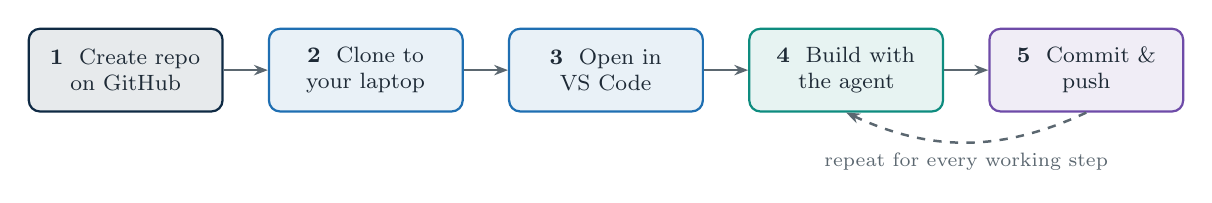
\begin{tikzpicture}[x=1cm,y=1cm]
    \node[step=cNavy,align=flush center] (s1) at (0,0) {\textbf{1}\ \ Create repo\\on GitHub};
    \node[step=cBlue,align=flush center] (s2) at (3.05,0) {\textbf{2}\ \ Clone to\\your laptop};
    \node[step=cBlue,align=flush center] (s3) at (6.1,0) {\textbf{3}\ \ Open in\\VS Code};
    \node[step=cTeal,align=flush center] (s4) at (9.15,0) {\textbf{4}\ \ Build with\\the agent};
    \node[step=cPurple,align=flush center] (s5) at (12.2,0) {\textbf{5}\ \ Commit \&\\push};
    \draw[arr] (s1) -- (s2); \draw[arr] (s2) -- (s3); \draw[arr] (s3) -- (s4); \draw[arr] (s4) -- (s5);
    \draw[arr,dashed] (s5.south) to[bend left=25] node[lbl,below=2pt]{repeat for every working step} (s4.south);
  \end{tikzpicture}
  \vspace{2pt}
  \begin{keybox}[Why this order?]
    \begin{itemize}\setlength{\itemsep}{1pt}
      \item README, \texttt{.gitignore} (template ``Python'') and licence\\are created on GitHub with one click
      \item the connection to GitHub exists from the start -- no \texttt{git remote add} later
      \item issues, branches and collaboration work from minute one
    \end{itemize}
  \end{keybox}
  \note{This order is the most robust one for beginners. On github.com: New repository, name it (e.g. \texttt{ai-automation-pocs}), tick ``Add a README'', choose the \texttt{.gitignore} template ``Python'', optionally a licence. Then clone it -- either with \texttt{git clone} in the terminal or in VS Code with the command ``Git: Clone'' / the Clone Repository button in the Source Control view.\par
  Private or public? For coursework, private is fine; students who want a portfolio can make it public later -- but then secrets must never have been committed (next slides).\par
  Alternative for students who already have a local folder: VS Code's ``Publish to GitHub'' button creates the remote repository afterwards.}
\end{frame}

% ------------------------------------------------------------------
\begin{frame}[fragile]{Git in practice}{Terminal commands -- or the same actions as buttons in VS Code}
  \vspace{2pt}
    \begin{columns}[T,onlytextwidth]
        \begin{column}{0.57\textwidth}
\begin{lstlisting}[language=bash,aboveskip=0pt,basicstyle=\ttfamily\footnotesize\color{cInk}]
# 1. copy the repository to your laptop (once)
git clone https://github.com/<user>/<repo>.git
cd <repo>

# 2. ... let the agent build, review, test ...

# 3. save a working step and upload it
git status                     # what changed?
git add .
git commit -m "POC 1: CSV upload and statistics"
git push
\end{lstlisting}
    \end{column}
            \begin{column}{0.40\textwidth}
      \begin{keybox}[Golden rule]
        Commit after \emph{every} change\\that works.
      \end{keybox}
      \vskip3pt % gap between stacked boxes: 6pt
      \begin{infobox}[Good commit messages]
        say \emph{what} works now:\\``POC 2: /api/upload\\stores metadata''\par
        \muted{not:} ``changes'', ``asdf''
      \end{infobox}
    \end{column}
  \end{columns}
  \takeaway{Commit small and often -- every commit is a save point you can go back to.}
  \note{Show both ways once: the terminal commands and the Source Control view in VS Code (stage with +, type the message, Commit, then Sync/Push). Copilot can also suggest a commit message from the diff (sparkle icon in the message box) -- students should still read it.\par
  Emphasise \texttt{git status} before \texttt{git add .}: it shows what would be committed. This is where students notice a \texttt{.env} file or a huge database that should not be committed.\par
  Tip for the POCs: commit after each item of the run-and-verify checklist. Small commits make it easy to find the step that broke something.}
\end{frame}

% ------------------------------------------------------------------
\begin{frame}[fragile]{One repository, three POCs}{Each POC is self-contained -- with its own environment and requirements}
  \vspace{2pt}
  \begin{columns}[T]
    \begin{column}{0.53\textwidth}
\begin{lstlisting}[basicstyle=\ttfamily\scriptsize,aboveskip=0pt,belowskip=0pt]
ai-automation-pocs/
|-- .gitignore      # what Git ignores
|-- README.md       # overview + start commands
|-- poc1_streamlit/
|   |-- .venv/      # local only (ignored)
|   |-- app.py
|   |-- sample_data.py
|   +-- requirements.txt
|-- poc2_fastapi_sqlite/
|   |-- backend/    # FastAPI + SQLite
|   |-- frontend/   # Streamlit
|   +-- requirements.txt
+-- poc3_xgboost_churn/   # like POC 2 + model
\end{lstlisting}
    \end{column}
    \begin{column}{0.43\textwidth}
      \begin{keybox}[Conventions]
        \begin{itemize}\setlength{\itemsep}{1pt}
          \item one repo, one folder per POC
          \item own \file{.venv} + \file{requirements.txt} per POC
                    \item root \file{README.md}\\with start commands
        \end{itemize}
      \end{keybox}
    \end{column}
      \end{columns}
  \vspace{3pt}
  \begin{warnbox}[What belongs in the repo?]
    Everything needed to rebuild the project elsewhere -- nothing generated, nothing secret.
  \end{warnbox}
  \note{One repository keeps everything in one place: easy to clone, one history, one README. Each POC gets its own folder, virtual environment and requirements file, so that packages of POC 3 (xgboost, scikit-learn) cannot break POC 1.\par
  The rule in the warning box is the most important one: the repository contains what is needed to reproduce the project on another machine -- source code, the list of dependencies, configuration templates and documentation. It does not contain what can be regenerated (virtual environments, databases, caches -- and large trained models) or what is secret (API keys, passwords, personal data).\par
  Ask: ``Where does the SQLite database of POC 2 belong?'' -- not in Git; it is created at start-up.}
\end{frame}

% ------------------------------------------------------------------
\begin{frame}[fragile]{\texttt{.gitignore}: what stays out of the repository}
  \vspace{2pt}
  \begin{columns}[T,onlytextwidth]
    \begin{column}{0.60\textwidth}
      {\small A text file in the repo root that tells Git which files and folders to \textbf{ignore}. Without it, repositories become bloated, slow -- and unsafe.}\par\vspace{6pt}
      {\small
      \begin{tabularx}{\linewidth}{@{}l Y@{}}
        \toprule
        \textbf{Entry} & \textbf{Why}\\
        \midrule
        \texttt{.venv/}, \texttt{\_\_pycache\_\_/} & local, machine-specific\\
        \texttt{*.db}, \texttt{data/uploads/} & generated at runtime\\
        \texttt{.env}, \texttt{*.key} & secrets -- once pushed = leaked\\
        \bottomrule
      \end{tabularx}}
    \end{column}
        \begin{column}{0.36\textwidth}
      \begin{card}[cTeal]{Example \texttt{.gitignore}}
\begin{lstlisting}[basicstyle=\ttfamily\footnotesize,backgroundcolor=\color{white},frame=none]
.venv/
__pycache__/
*.db
data/uploads/
.env
*.key
.streamlit/secrets.toml
\end{lstlisting}
      \end{card}
    \end{column}
  \end{columns}
  \takeaway{Check \texttt{.gitignore} \emph{before} the first commit --\\ignoring a file later does not remove it from history.}
  \note{GitHub's ``Python'' template (selected when creating the repository) already covers \texttt{.venv}, \texttt{\_\_pycache\_\_}, \texttt{.env} and Streamlit's \texttt{secrets.toml}. Trained model files can be committed in a POC if they are small; large ones belong elsewhere.\par
  Important subtlety from the Git documentation: \texttt{.gitignore} only affects untracked files. If a file was committed before it was added to \texttt{.gitignore}, Git keeps tracking it -- and it remains in the history. That is why the check must happen before the first commit.\par
  Note: GitHub's Python template ignores Django's \texttt{db.sqlite3}, but not \texttt{*.db} or \texttt{app.db} -- add them. Nice detail: since Python 3.13, \texttt{python -m venv} automatically places a \texttt{.gitignore} inside the new \texttt{.venv} folder.}
\end{frame}

% ------------------------------------------------------------------
\begin{frame}[fragile]{Secrets and security}{API keys and passwords never go into code or Git}
  \vspace{2pt}
  \begin{columns}[T]
    \begin{column}{0.48\textwidth}
      \begin{badbox}[Never in the repository]
        API keys, tokens, passwords, \file{.env} files with real values, databases with personal data
      \end{badbox}
      \vskip3pt % gap between stacked boxes: 6pt
      \begin{keybox}[Instead]
        Keep secrets in a local \file{.env} (ignored). Commit a \file{.env.example}\\with empty placeholders.
\begin{lstlisting}[language=bash,backgroundcolor=\color{white}]
# .env.example
LLM_API_KEY=
\end{lstlisting}
      \end{keybox}
    \end{column}
    \begin{column}{0.48\textwidth}
      \begin{warnbox}[If it happened anyway]
        \begin{enumerate}\setlength{\itemsep}{1pt}
          \item \textbf{revoke or rotate the key at once} (course key: tell the lecturer) -- deleting the file is not enough
          \item then clean the history \mbox{(\texttt{git filter-repo})} or ask for help
        \end{enumerate}
      \end{warnbox}
      \vskip3pt % gap between stacked boxes: 6pt
      \begin{infobox}[GitHub helps a little]
        Secret scanning and push protection catch many known key formats in public repos -- but not all.
      \end{infobox}
    \end{column}
  \end{columns}
  \note{The POCs of this deck need no secrets, but the prototypes in the LLM deck do -- for example the course API key that students receive by email. Establish the habit now.\par
  GitHub's documentation (as of Sep 2026) is explicit: if a secret was committed, ``as a first step you need to revoke and/or rotate that secret'' -- that may even be sufficient. Students cannot rotate the course API key themselves: if it leaks, they tell the lecturer at once so that it can be replaced for everyone. Rewriting history is the second step; GitHub now recommends \texttt{git-filter-repo} (a separate install, version 2.47 or later) with the \texttt{--sensitive-data-removal} option. Bots scan public GitHub repositories for keys within minutes, so rotating is urgent.\par
  Secret scanning runs automatically on public repositories, and push protection for users is on by default -- it blocks pushes containing recognised secrets to public repos. It does not cover every format and typically not private student repositories, so it is a safety net, not a strategy.}
\end{frame}

% ------------------------------------------------------------------
\begin{frame}[fragile]{Virtual environments}{Every project gets its own, isolated set of packages}
  \vspace{2pt}
  \begin{columns}[T]
    \begin{column}{0.47\textwidth}
      \begin{infobox}[Why?]
        Projects need different packages and versions. A \file{.venv} keeps them apart and makes \file{requirements.txt} reproducible.
      \end{infobox}
      \vskip3pt % gap between stacked boxes: 6pt
      \begin{keybox}[In VS Code]
        \kbd{Ctrl+Shift+P} $\rightarrow$\\\mbox{\emph{Python: Create Environment}}\\or \mbox{\emph{Python: Select Interpreter}}
      \end{keybox}
    \end{column}
    \begin{column}{0.49\textwidth}
\begin{lstlisting}[language=bash,aboveskip=0pt]
# create (once per project)
python3.13 -m venv .venv       # macOS / Linux
py -V:3.13 -m venv .venv       # Windows

# activate (every new terminal)
source .venv/bin/activate      # macOS / Linux
.venv\Scripts\Activate.ps1     # Windows

# install: by name, or all from the list
pip install streamlit pandas
pip install -r requirements.txt
\end{lstlisting}
    \end{column}
  \end{columns}
  \takeaway{The terminal line starts with \texttt{(.venv)}? Then you are in the right environment.}
  \note{A virtual environment is a folder containing its own Python interpreter and packages. Activating it changes which \texttt{python} and \texttt{pip} the terminal uses -- recognisable by the \texttt{(.venv)} prefix in the terminal prompt. VS Code's Python extension detects \texttt{.venv} folders and activates them in new terminals automatically once selected as interpreter.\par
  \texttt{requirements.txt} lists the packages a project needs; \texttt{pip install -r requirements.txt} recreates the environment on any machine. We let the agent maintain this file -- students should check that it contains what the code imports.\par
  Conda environments also work, but venv is built into Python and is what the agent expects by default. uv is a much faster Rust-based alternative (\texttt{uv venv}, \texttt{uv pip install}) -- optional for curious students.}
\end{frame}

% ------------------------------------------------------------------
\begin{frame}{Anatomy of a good coding prompt}{Six building blocks that turn generic code into \emph{your} code}
  \vspace{2pt}
  \begin{columns}[T]
    \begin{column}{0.50\textwidth}
      \begin{enumerate}\setlength{\itemsep}{3pt}\small
        \item \textbf{Goal} -- what should work, for whom
        \item \textbf{Stack} -- FastAPI + SQLAlchemy + SQLite
        \item \textbf{Files} -- \file{backend/main.py}, \file{frontend/app.py}
        \item \textbf{Interfaces \& output} -- tables, endpoints, JSON fields, UI elements
        \item \textbf{Demo data} -- \file{sample\_data.py},\\sample button
        \item \textbf{Done-criteria} -- ``done when \ldots'',\\packages, ports
      \end{enumerate}
    \end{column}
    \begin{column}{0.46\textwidth}
      \begin{keybox}[Why each block matters]
        Every block you leave out is a decision the agent makes for you -- usually the most generic one.
      \end{keybox}
      \vskip3pt % gap between stacked boxes: 6pt
      \begin{infobox}[Done-criteria example]
        ``Done when \texttt{streamlit run app.py} starts without errors and every numeric column has a histogram.''
      \end{infobox}
    \end{column}
  \end{columns}
  \takeaway{Bad prompts produce generic code. Good prompts produce \emph{your} code.}
  \note{This is the central slide of the method. The sixth block, explicit done-criteria, is the one beginners forget most often: telling the agent how success will be checked makes it test its own work and reduces ``finished'' code that does not run.\par
  Link to management practice: a good prompt is like a good work order or user story -- goal, context, deliverables, acceptance criteria. Business students already know this structure.\par
  Exercise (3 minutes): students rewrite the demo prompt from Session 1 and mark each of the six blocks in a different colour. Which block was missing? (Usually explicit done-criteria and constraints.)}
\end{frame}

% ------------------------------------------------------------------
\begin{frame}{From a vague to a specific prompt}
  \vspace{2pt}
  \begin{badbox}[Vague prompt -- leads to generic code]
    \ttfamily\footnotesize Build me an app that can analyse CSVs and does a bit of ML.
  \end{badbox}
  \vspace{2pt}
    % the building-block chips sit next to the part of the prompt they label
  \begin{keybox}[Specific prompt -- leads to \emph{your} code]
    \footnotesize\renewcommand{\arraystretch}{1.15}%
    \begin{tabularx}{\linewidth}{@{}Y r@{}}
      Create \texttt{backend/} with FastAPI + SQLAlchemy + SQLite. & \pill[cBlue]{GOAL} \pill[cTeal]{STACK} \pill[cNavy]{FILES}\\
      Models: \texttt{Upload}, \texttt{AnalysisRun}, \texttt{ColumnStat}. Endpoints: \texttt{POST /api/upload}, \texttt{GET /api/uploads}, \texttt{POST /api/analyze/\{id\}}. Pydantic schemas for all responses. & \pill[cPurple]{INTERFACES}\\
      Demo data via \texttt{sample\_data.py}. & \pill[cOrange]{DEMO DATA}\\
      Done when all endpoints work in \texttt{/docs} with the sample upload. & \pill[cGreen]{DONE-CRITERIA}\\
    \end{tabularx}
  \end{keybox}
  \takeaway{The second prompt is longer -- and saves you three rounds of corrections.}
  \note{Read both prompts aloud. Say explicitly that the technical words (FastAPI, SQLAlchemy, Pydantic, endpoints, \texttt{/docs}) are the POC 2 vocabulary of Parts 4 and 6 -- today only the \emph{structure} matters. Ask the students to predict what the agent will do with the first one: it has to guess the framework, the file structure, the data model, where the data comes from and when it is finished -- and it will guess differently every time.\par
  The second prompt names the stack, the files, the data model, the endpoints, the demo data and a done-criterion. Two agents given this prompt will produce very similar, predictable projects. That is what we want for learning -- and for business applications.\par
  Students who have seen web tutorials may expect CORS middleware here. For a Streamlit frontend this is unnecessary -- Streamlit calls the API from Python on the server, not from the browser. We explain why in Part 4.}
\end{frame}

% ------------------------------------------------------------------
\begin{frame}[fragile]{Project instructions: tell the agent your rules once}{A Markdown file that Copilot reads with every chat request in this repository}
  \vspace{2pt}
  \begin{columns}[T]
    \begin{column}{0.55\textwidth}
      \begin{card}[cNavy]{\texttt{.github/copilot-instructions.md}}
\begin{lstlisting}[basicstyle=\ttfamily\scriptsize,backgroundcolor=\color{white},frame=none,aboveskip=0pt,belowskip=0pt]
# Rules for this repository
- Python 3.13, one .venv per POC folder.
- Keep code simple and commented for
  business students.
- Ask before adding a new dependency;
  keep requirements.txt up to date.
- Never hard-code secrets; use .env.
- After each change: explain it in
  3-5 bullets and update the README
  run commands.
\end{lstlisting}
      \end{card}
    \end{column}
    \begin{column}{0.41\textwidth}
      \begin{keybox}[Why?]
        Conventions you would otherwise repeat in every prompt -- stated once, applied always.
      \end{keybox}
      \vskip3pt % gap between stacked boxes: 6pt
      \begin{infobox}[Alternatives]
        \file{AGENTS.md} in the repo root works too. The chat command \texttt{/init} drafts a starter file for you.
      \end{infobox}
    \end{column}
  \end{columns}
  \takeaway{Create this file in your repository now --\\short, concrete house rules the agent reads in every POC.}
  \note{Custom instructions are supported in VS Code for the Copilot harness (docs, Sep 2026): \texttt{.github/copilot-instructions.md} for the whole repository, \texttt{.github/instructions/*.instructions.md} for rules that apply only to certain files (\texttt{applyTo} patterns), and \texttt{AGENTS.md}, an open format that several coding agents understand. The chat command \texttt{/init} generates a starter file from the existing project.\par
  Have students create the file now -- copy the example or run \texttt{/init} and trim the result -- and commit it; the POC steps assume it exists. Good instruction files are short: coding conventions, environment, what to ask before doing, how to report changes. Long, vague instructions are ignored or cause confusion.\par
  Older tutorials also mention reusable ``prompt files'' (\texttt{.prompt.md}); these are deprecated for Copilot sessions and replaced by ``agent skills'' -- not needed in this course.}
\end{frame}

% ------------------------------------------------------------------
\begin{frame}{Plan first, then build}{For every step that touches more than one file}
  \centering
  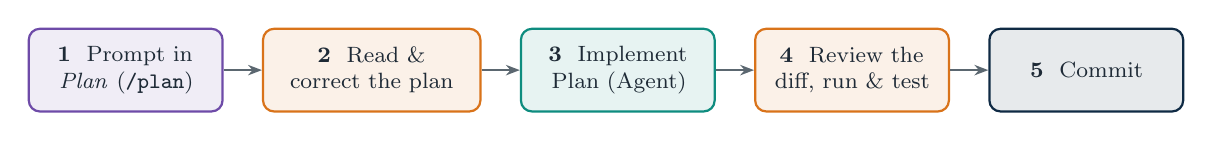
\begin{tikzpicture}[x=1cm,y=1cm]
    \node[step=cPurple,align=flush center] (a) at (0,0) {\textbf{1}\ \ Prompt in\\\emph{Plan} (\texttt{/plan})};
    \node[step=cOrange,minimum width=2.75cm,text width=2.55cm,align=flush center] (b) at (3.125,0) {\textbf{2}\ \ Read \&\\correct the plan};
    \node[step=cTeal,align=flush center] (c) at (6.25,0) {\textbf{3}\ \ Implement\\Plan (Agent)};
    \node[step=cOrange,align=flush center] (d) at (9.225,0) {\textbf{4}\ \ Review the\\diff, run \& test};
    \node[step=cNavy,align=flush center] (e) at (12.2,0) {\textbf{5}\ \ Commit};
    \draw[arr] (a) -- (b); \draw[arr] (b) -- (c); \draw[arr] (c) -- (d); \draw[arr] (d) -- (e);
  \end{tikzpicture}
  \par\vspace{8pt}
  \begin{columns}[T]
    \begin{column}{0.48\textwidth}
            % keybox / infobox look with equal heights
      \begin{tcolorbox}[aidabase,colback=cTealL,borderline west={3pt}{0pt}{cTeal},equal height group=d1aPlan]
        {\color{cTeal}\bfseries What to look for in a plan}\par\vspace{1pt}
        right files? right stack? no surprise dependencies? steps you understand? a way to test?
      \end{tcolorbox}
    \end{column}
    \begin{column}{0.48\textwidth}
            \begin{tcolorbox}[aidabase,colback=cBlueL,borderline west={3pt}{0pt}{cBlue},equal height group=d1aPlan]
        {\color{cBlue}\bfseries Correct in plain language}\par\vspace{1pt}
        ``Use SQLite, not PostgreSQL. Put the API in \texttt{backend/}. Skip authentication.''
      \end{tcolorbox}
    \end{column}
  \end{columns}
  \takeaway{Correcting a plan costs one sentence; correcting finished code costs an afternoon.}
  \note{The Plan mode researches the task and proposes a structured implementation plan before any file is changed (VS Code docs). In Copilot sessions: \texttt{/plan} or the mode selector; the plan card offers \emph{Implement Plan} (in Local sessions: \emph{Start Implementation}). Students review it like a project manager reviews a work plan: are the files and technologies right, is anything unexpected included, can I test the result?\par
  Orange boxes again mark human decisions. Steps 2 and 4 are where students learn most -- insist that they read the plan and the diff (VS Code's side-by-side view of old and new lines for every file the agent changed), even if it feels slow at first.\par
  For very small changes (``rename the button'', ``add a title'') going directly to Agent is fine. Rule of thumb: more than one file or a new dependency $\rightarrow$ plan first.}
\end{frame}

% ------------------------------------------------------------------
\begin{frame}{Three-stage review for AI-generated code}
  \vspace{2pt}
  \begin{columns}[T,onlytextwidth]
    \begin{column}{0.315\textwidth}
      \begin{card}[cBlue]{\numdot[cNavy]{1}\ \ Read \& understand}[equal height group=rev]
        Do I understand \emph{every} changed line? If not: ask in Ask -- ``explain lines 12--18'' -- \emph{then} accept. Use the diff view.
      \end{card}
    \end{column}
    \begin{column}{0.315\textwidth}
      \begin{card}[cTeal]{\numdot[cNavy]{2}\ \ Run \& test}[equal height group=rev]
        Start the app. Try the normal case (``happy path'') \emph{and} at least one error case: empty CSV, wrong file type, missing~field.
      \end{card}
    \end{column}
    \begin{column}{0.315\textwidth}
      \begin{card}[cOrange]{\numdot[cNavy]{3}\ \ Hallucination check}[equal height group=rev]
        Do the packages exist? Does \texttt{pip install} work? Are paths, ports and parameters consistent?
      \end{card}
    \end{column}
  \end{columns}
  \takeaway{Read it, run it, check it -- only then commit it.}
  \note{This three-stage review is the single most important habit of the course. Stage 1 protects against code you cannot maintain or explain; stage 2 against code that looks right but fails; stage 3 against the specific failure modes of language models.\par
  For stage 2, error cases are key: an empty file, a CSV with text in a numeric column, a missing value. Agents tend to write code for the happy path only. Asking ``what happens if the CSV is empty? Add handling and a friendly message'' is an excellent follow-up prompt.\par
  Link to the evidence slide: the METR study showed that experienced developers overestimated the benefit of AI. Structured review keeps our judgement honest.}
\end{frame}

% ------------------------------------------------------------------
\begin{frame}{Typical hallucinations in AI-generated code}{Plausible-looking, but wrong}
  \vspace{2pt}
  \begin{columns}[T]
    \begin{column}{0.55\textwidth}
      \begin{warnbox}[Symptoms]
        \begin{itemize}\setlength{\itemsep}{1pt}
          \item invented packages $\rightarrow$ \texttt{ModuleNotFoundError}
          \item non-existent functions, outdated APIs
          \item plausible but wrong defaults\\or column names
          \item gaps: \texttt{\# implementation here}
          \item ``it works'' -- without having run it
        \end{itemize}
      \end{warnbox}
    \end{column}
    \begin{column}{0.41\textwidth}
      \begin{badbox}[A security angle]
        Don't install a package just because the AI named it -- attackers register look-alike names. Check \texttt{pypi.org} first.
      \end{badbox}
      \vskip3pt % gap between stacked boxes: 6pt
      \begin{keybox}[Countermeasure]
        Paste the full error back and ask the agent to fix the \emph{cause}.
      \end{keybox}
    \end{column}
  \end{columns}
  \takeaway{If the code sounds too good -- install and run it first, \emph{then} believe it.}
  \note{Why hallucinations happen: the model generates the most plausible continuation, not a verified one (the LLM deck explains why in Parts 1 and 3). Package and function names that ``sound right'' are especially risky, because they often existed in older versions or in similar libraries.\par
  The security point: if a model repeatedly suggests a package that does not exist, an attacker can register exactly that name on PyPI with malicious code. This supply-chain risk is sometimes called ``slopsquatting''. Checking the package page (maintainer, downloads, documentation) before installing is a cheap defence.\par
  Good news for the POCs: we use only very popular libraries (pandas, Streamlit, FastAPI, SQLAlchemy, XGBoost), so hallucinated packages are rare -- but outdated API usage still happens, e.g. deprecated FastAPI start-up events or old SQLAlchemy syntax.}
\end{frame}

% ------------------------------------------------------------------
\begin{frame}{Top pitfalls -- and how to avoid them}
  \vspace{2pt}
  {\footnotesize
  \renewcommand{\arraystretch}{1.5}
  \begin{tabularx}{\textwidth}{@{}c L{4.9cm} Y@{}}
    \toprule
    & \textbf{Pitfall} & \textbf{Prevention}\\
    \midrule
    \numdot{1} & wrong Python environment & \texttt{(.venv)} in the terminal; \emph{Python: Select Interpreter}\\
    \numdot{2} & secrets in the repository & \file{.env} in \file{.gitignore} before the first commit\\
    \numdot{3} & ``connection refused'' in POC 2/3 & the backend is not running -- start it in a second terminal\\
    \numdot{4} & port already in use (8000 / 8501) & stop the old process (\kbd{Ctrl+C}) or use another port\\
    \numdot{5} & huge, unexplained changes & plan first; one feature per prompt; ask for a summary\\
    \numdot{6} & no commits for hours & commit after every working step\\
    \bottomrule
  \end{tabularx}}
  \takeaway{Setup before code: most problems appear before the first prompt --\\or when two processes must talk.}
  \note{These are the pitfalls beginners hit most often in POC sessions. One item that many online tutorials list is missing on purpose: ``CORS errors'' do not occur in our architecture. CORS is a browser security rule for JavaScript that calls an API on another origin; Streamlit calls FastAPI from its Python code on the server, so the browser is not involved (MDN; FastAPI docs). CORS becomes relevant only if a JavaScript frontend such as React calls the API directly.\par
  Pitfall 3 is the classic in POC 2: students start only the Streamlit app and get ``connection refused'' because nothing listens on port 8000. The fix is two terminals, one per process -- we practise this in Part 6.\par
  Ask students which pitfall they already hit in Session 1.}
\end{frame}
% ==================================================================
% PART 4 -- FOUNDATIONS: HOW APPS ARE BUILT
% ==================================================================
\section{How apps are built}
\partframe{Session 2 and following}{Frontend, backend, database -- the vocabulary every automation project uses.}{%
  \darkitem{Explain the three-tier architecture with an everyday analogy}
  \darkitem{Follow a click from the browser to the database and back}
  \darkitem{Read an HTTP request, a JSON response and a simple SQL query}
  \darkitem{Know what runs where: processes, ports, localhost}}

% ------------------------------------------------------------------
\begin{frame}{The three-tier architecture}{Almost every business application is built in three layers}
  \vspace{2pt}
  \begin{columns}[T]
    \begin{column}{0.66\textwidth}
      \centering
      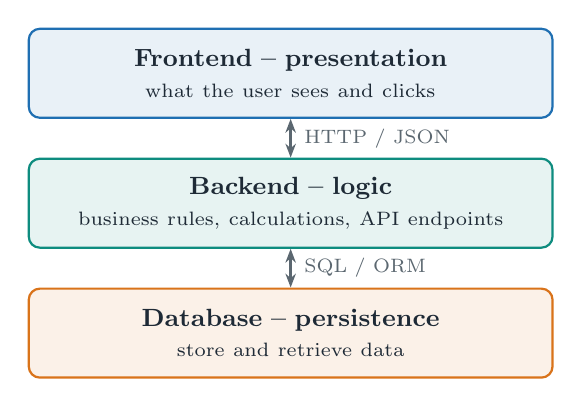
\begin{tikzpicture}[x=1cm,y=1cm]
        \node[lay=cBlue,minimum width=6.6cm,text width=6.3cm,minimum height=1.13cm] (fe) at (0,2.3) {\textbf{Frontend -- presentation}\\\scriptsize what the user sees and clicks};
        \node[lay=cTeal,minimum width=6.6cm,text width=6.3cm,minimum height=1.13cm] (be) at (0,0.65) {\textbf{Backend -- logic}\\\scriptsize business rules, calculations, API endpoints};
        \node[lay=cOrange,minimum width=6.6cm,text width=6.3cm,minimum height=1.13cm] (db) at (0,-1.0) {\textbf{Database -- persistence}\\\scriptsize store and retrieve data};
        \draw[darr] (fe) -- node[lbl,right=3pt]{HTTP / JSON} (be);
        \draw[darr] (be) -- node[lbl,right=3pt]{SQL / ORM} (db);
      \end{tikzpicture}
    \end{column}
    \begin{column}{0.31\textwidth}
      \begin{graybox}[\faUtensils\ \ Restaurant analogy]
        \textbf{Dining room} = frontend\\
        \textbf{Kitchen} = backend\\
        \textbf{Pantry} = database\\[3pt]
        The waiter (API) carries orders in a fixed format.
      \end{graybox}
      {\scriptsize\muted{Typical tools:\\ Streamlit, React\\ FastAPI, Django\\ SQLite, PostgreSQL}\par}
    \end{column}
  \end{columns}
  \takeaway{Architecture answers one question: who calls whom, how -- and who stores what.}
  \note{The restaurant analogy works well with business students: guests never walk into the kitchen; they order through a waiter using the menu (a fixed format). The kitchen can change its recipes or staff without redesigning the dining room, and the pantry can be reorganised without the guests noticing.\par
  Translate back: the frontend (Streamlit in our POCs) only shows data and collects input; the backend (FastAPI) contains the business logic and exposes it through an API; the database (SQLite) stores data permanently. Gloss the arrow labels: an endpoint is one address of the API (a path such as \texttt{/api/upload} plus GET or POST); an ORM is a library that writes the SQL for us from Python objects -- both get their own slide shortly.\par
  Note that the layers are a logical separation. In POC 1 all three live in one Streamlit script; in POC 2 they become separate programs. Seeing the same app in both shapes is the key learning of POC 1 vs.\ POC 2.}
\end{frame}

% ------------------------------------------------------------------
\begin{frame}{What happens when you click a button?}{One request through all three layers (POC 2)}
  \centering
  \begin{tikzpicture}[x=1cm,y=1cm]
    \foreach \x/\c/\t/\i/\n in {0.9/cBlue/Browser/\faDesktop/b,5.0/cBlue/Streamlit/\faChartBar/s,9.1/cTeal/FastAPI/\faServer/f,13.2/cOrange/SQLite/\faDatabase/d}
      {\node[sbox=\c,minimum width=2.1cm,minimum height=0.55cm,font=\scriptsize\bfseries] (\n) at (\x,0) {\i\ \ \t};
       \draw[cLine,line width=1pt,dashed] (\x,-0.3) -- (\x,-4.05);}
    \draw[arr,cBlue] (0.9,-0.75) -- node[lbl,above]{\textbf{1}\ click ``Run analysis''} (5.0,-0.75);
    \draw[arr,cTeal] (5.0,-1.35) -- node[lbl,above]{\textbf{2}\ \texttt{POST /api/analyze/3}} (9.1,-1.35);
    \draw[arr,cOrange] (9.1,-1.95) -- node[lbl,above]{\textbf{3}\ \texttt{SELECT} \ldots / \texttt{INSERT} \ldots} (13.2,-1.95);
    \draw[arr,dashed,cOrange] (13.2,-2.55) -- node[lbl,above]{\textbf{4}\ rows} (9.1,-2.55);
    \draw[arr,dashed,cTeal] (9.1,-3.15) -- node[lbl,above]{\textbf{5}\ \texttt{200 OK} + JSON} (5.0,-3.15);
    \draw[arr,dashed,cBlue] (5.0,-3.75) -- node[lbl,above]{\textbf{6}\ updated page} (0.9,-3.75);
  \end{tikzpicture}
  \par\vspace{2pt}
  {\scriptsize\muted{Browser $\leftrightarrow$ Streamlit: WebSocket \quad\textbullet\quad Streamlit $\leftrightarrow$ FastAPI: HTTP \quad\textbullet\quad FastAPI $\leftrightarrow$ SQLite: SQL via SQLAlchemy}}
  \takeaway{Every layer only talks to its neighbour -- that is what makes each one replaceable.}
  \note{Walk through the six steps slowly; this picture is the mental model for POC 2 and POC 3. (1) The user clicks a button; the browser tells the Streamlit server via its WebSocket connection. (2) The Streamlit script -- running on the server -- sends an HTTP request to FastAPI. (3) FastAPI runs the business logic and queries or writes the database through SQLAlchemy. (4) The database returns rows. (5) FastAPI answers with status code 200 and a JSON body. (6) Streamlit reruns the script and sends the updated page to the browser.\par
  Important detail: the browser never talks to FastAPI directly in our setup -- that is why CORS plays no role (it is a browser rule). Ask: ``Where would you look first if step 2 fails?'' (Is the backend running? Is the URL correct?)}
\end{frame}

% ------------------------------------------------------------------
\begin{frame}[fragile]{HTTP in one slide}{The language in which frontends and backends talk}
  \vspace{2pt}
  \begin{columns}[T,onlytextwidth]
    \begin{column}{0.485\textwidth}
      {\small\bfseries\color{cNavy}Methods -- what you want}\par\vspace{2pt}
      {\footnotesize
      \renewcommand{\arraystretch}{1.3}%
      \begin{tabular}{@{}l L{4.8cm}@{}}
        \toprule
        \pill[cBlue]{GET} & retrieve data (no changes)\\
        \pill[cTeal]{POST} & submit data, create something\\
        \pill[cOrange]{PUT} & replace an existing resource\\
        \pill[cRed]{DELETE} & delete a resource\\
        \bottomrule
      \end{tabular}}
      \par\vspace{6pt}
      {\small\bfseries\color{cNavy}A request}
\begin{lstlisting}[language=bash]
POST http://localhost:8000/api/predict
Content-Type: application/json

{"tenure_months": 3, "monthly_charges": 79.9}
\end{lstlisting}
    \end{column}
    \begin{column}{0.485\textwidth}
      {\small\bfseries\color{cNavy}Status codes -- what happened}\par\vspace{2pt}
      {\footnotesize
      \begin{tabular}{@{}l L{3.9cm}@{}}
        \toprule
        \textbf{200} OK & success\\
        \textbf{201} Created & new resource created\\
        \textbf{400} Bad Request & the request is malformed\\
        \textbf{404} Not Found & wrong path or unknown ID\\
        \textbf{422} Unprocessable & valid JSON, wrong fields/types\\
        \textbf{500} Server Error & bug in the backend\\
        \bottomrule
      \end{tabular}}
      \par\vspace{6pt}
      \begin{keybox}
        \textbf{2xx} = fine\\
        \textbf{4xx} = the caller made a mistake\\
        \textbf{5xx} = the server did
      \end{keybox}
    \end{column}
  \end{columns}
  \source{MDN Web Docs (HTTP methods, status codes)}
  \note{HTTP is the protocol of the web. Every request has a method, a URL (address + path) and optionally a body -- in our case JSON. Every response has a status code and usually a JSON body.\par
  The method semantics follow MDN: GET should only retrieve data; POST submits data and often changes state; PUT replaces a resource; DELETE removes it. GET, PUT and DELETE are idempotent (repeating them has the same effect), POST is not -- that is why browsers warn before re-submitting a form.\par
  422 (``Unprocessable Content'') is the code students will see most in POC 2 and 3: FastAPI returns it automatically when the JSON does not match the Pydantic schema -- for example a missing field or text instead of a number -- and, in FastAPI, also for malformed JSON. The response body tells you exactly which field is wrong.}
\end{frame}

% ------------------------------------------------------------------
\begin{frame}[fragile]{An API is a contract}{Both sides agree on paths, fields and types -- and can then evolve independently}
  \vspace{2pt}
  \begin{columns}[T]
    \begin{column}{0.48\textwidth}
      \begin{card}[cBlue]{Request (frontend $\rightarrow$ backend)}[equal height group=contract]
\begin{lstlisting}[language=JSON,backgroundcolor=\color{white},frame=none,xleftmargin=0pt,framexleftmargin=0pt]
POST /api/predict
{
  "age": 34,
  "tenure_months": 7,
  "monthly_charges": 74.9,
  "contract_type": "monthly"
}
\end{lstlisting}
      \end{card}
    \end{column}
    \begin{column}{0.48\textwidth}
      \begin{card}[cTeal]{Response (backend $\rightarrow$ frontend)}[equal height group=contract]
\begin{lstlisting}[language=JSON,backgroundcolor=\color{white},frame=none,xleftmargin=0pt,framexleftmargin=0pt]
200 OK
{
  "churn_probability": 0.71,
  "prediction": 1,
  "model_run_id": 3
}
\end{lstlisting}
      \end{card}
    \end{column}
  \end{columns}
  \addvspace{6pt}
  \begin{keybox}
    FastAPI turns this contract into a live, clickable documentation page at \texttt{/docs}.
  \end{keybox}
  \takeaway{Agree on the contract first -- then build (and prompt) both sides separately.}
  \note{An API (application programming interface) is a promise: ``if you send me this JSON to this path, I will answer with that JSON.'' As long as the contract stays the same, the frontend team can redesign the user interface and the backend team can replace the model -- neither needs to know the other's code.\par
  This is also why we write two separate prompts in POC 2 (backend, frontend): the endpoint list and the JSON fields are the contract that connects them. If the fields in the two prompts do not match, the app breaks with 422 errors.\par
  JSON in one sentence: text with key--value pairs in curly braces, lists in square brackets; values are strings, numbers, true/false, null or nested objects. The example is POC 3's prediction endpoint with illustrative values; POC 2's endpoints follow the same pattern. An HTTP API built like this -- paths, GET/POST, JSON -- is what people call a REST API.}
\end{frame}

% ------------------------------------------------------------------
\begin{frame}{Frontend vs.\ backend -- and where Streamlit sits}
  \vspace{2pt}
  \begin{columns}[T]
    \begin{column}{0.52\textwidth}
      {\footnotesize
      \renewcommand{\arraystretch}{1.25}
      \begin{tabularx}{\linewidth}{@{}l Y Y@{}}
        \toprule
        & \textbf{Frontend} & \textbf{Backend}\\
        \midrule
        Job & show data, collect input & rules, calculations, data access\\
        Talks to & the user & database, models, other systems\\
        Must be & easy to use & correct, secure, reliable\\
        In POC 2/3 & Streamlit & FastAPI\\
        \bottomrule
      \end{tabularx}}
    \end{column}
    \begin{column}{0.44\textwidth}
      \begin{infobox}[Streamlit is special]
        You write only Python. The script runs \textbf{on the server}; the browser just displays the result and sends clicks back (WebSocket).
      \end{infobox}
      \addvspace{5pt}
      \begin{keybox}[Consequence]
        Uploaded data and the app's session values (\texttt{st.session\_state}) live in the \textbf{server's memory} -- one session per browser tab.
      \end{keybox}
    \end{column}
  \end{columns}
  \takeaway{Streamlit gives you a frontend without HTML or JavaScript -- ideal for data prototypes.}
  \note{In classic web development the frontend is HTML, CSS and JavaScript running in the browser (e.g. React). Streamlit takes a different approach, according to its architecture documentation: the Python script is the server; the browser is only a client connected through a WebSocket. Each browser tab gets its own session, and the script reruns from top to bottom on every interaction.\par
  A common misconception is that the data lives in the ``browser session state'': in fact \texttt{st.session\_state} is stored on the server per session -- if the Streamlit server restarts, it is gone.\par
  Business consequence: Streamlit is excellent for internal data tools and prototypes; for customer-facing products with many users, companies usually build a JavaScript frontend -- and then CORS becomes relevant.}
\end{frame}

% ------------------------------------------------------------------
\begin{frame}[fragile]{Databases in five minutes}{Tables, SQL -- and an ORM that writes SQL for you}
  \vspace{2pt}
  \begin{columns}[T]
    \begin{column}{0.49\textwidth}
      {\small\bfseries\color{cNavy}Table \texttt{uploads}}\par\vspace{2pt}
      {\footnotesize
      \begin{tabular}{@{}r l r r@{}}
        \toprule
        \textbf{id} & \textbf{filename} & \textbf{n\_rows} & \textbf{n\_cols}\\
        \midrule
        1 & sample.csv & 500 & 8\\
        2 & sales\_q3.csv & 1\,204 & 12\\
        \bottomrule
      \end{tabular}}
      \par\vspace{2pt}
      {\scriptsize\muted{\textbf{id} = primary key: unique for every row}}
      \par\vspace{4pt}
      {\small\bfseries\color{cNavy}SQL: ask the database}
\begin{lstlisting}[language=SQL]
SELECT filename, n_rows FROM uploads
WHERE n_rows > 1000;
\end{lstlisting}
    \end{column}
    \begin{column}{0.47\textwidth}
      \begin{infobox}[SQLite]
        a complete SQL database in a \textbf{single file} (\file{app.db}) -- no server, no configuration, part of Python.
      \end{infobox}
      \addvspace{5pt}
      \begin{keybox}[ORM (SQLAlchemy)]
        maps Python classes to tables: \texttt{Upload(filename=\ldots)} becomes a row~-- the ORM writes the SQL.
      \end{keybox}
    \end{column}
  \end{columns}
  \takeaway{Tables store facts, SQL asks questions, the ORM lets Python do both.}
  \note{A relational database stores data in tables: each row is a record (one upload), each column an attribute. The primary key identifies each row uniquely; other tables refer to it (e.g. \texttt{analysis\_runs.upload\_id}) -- that is the ``relational'' part.\par
  SQL is the standard query language; the example selects all uploads with more than 1,000 rows. Business students often know SQL-like queries from Excel filters or BI tools -- make that link.\par
  SQLite describes itself as a ``self-contained, serverless, zero-configuration, transactional SQL database engine'' stored in a single file, and as the most widely deployed database engine; Python ships the \texttt{sqlite3} module. SQLAlchemy is an ORM (object-relational mapper): we define Python classes, and it creates tables and SQL statements. In production, companies swap SQLite for PostgreSQL -- with an ORM mainly a change of the connection string, plus a database driver (e.g. psycopg) and a migration tool (e.g. Alembic).}
\end{frame}

% ------------------------------------------------------------------
\begin{frame}[fragile]{Processes, ports and localhost}{Two programs, two terminals, two addresses}
  \vspace{2pt}
  \begin{columns}[T]
    \begin{column}{0.49\textwidth}
      \begin{card}[cTeal]{\faTerminal\ \ Terminal 1 -- backend}[equal height group=term]
\begin{lstlisting}[language=bash,backgroundcolor=\color{white},frame=none,xleftmargin=0pt,framexleftmargin=0pt]
uvicorn backend.main:app --reload
# -> http://127.0.0.1:8000
\end{lstlisting}
      \end{card}
    \end{column}
    \begin{column}{0.47\textwidth}
      \begin{card}[cBlue]{\faTerminal\ \ Terminal 2 -- frontend}[equal height group=term]
\begin{lstlisting}[language=bash,backgroundcolor=\color{white},frame=none,xleftmargin=0pt,framexleftmargin=0pt]
streamlit run frontend/app.py
# -> http://localhost:8501
\end{lstlisting}
      \end{card}
    \end{column}
  \end{columns}
  \vspace{10pt}
  {\footnotesize
  \renewcommand{\arraystretch}{1.25}
  \begin{tabularx}{\textwidth}{@{}l Y@{}}
    \toprule
    \textbf{process} & a running program -- it keeps running until you stop it with \kbd{Ctrl+C}\\
    \textbf{localhost} (= \texttt{127.0.0.1}) & ``this computer''. FastAPI listens only there; Streamlit also shows a \emph{Network URL}\\
    \textbf{port} & a numbered door of the computer: Streamlit 8501, FastAPI 8000 by default\\
    \bottomrule
  \end{tabularx}}
  \takeaway{Both processes must run at the same time -- one terminal each.}
  \note{Students often think of an app as one thing. In POC 2 it is two programs: FastAPI served by Uvicorn (default address 127.0.0.1, port 8000) and Streamlit (default port 8501). Each needs its own terminal; closing the terminal or pressing Ctrl+C stops the process.\par
  Localhost means the computer you are sitting at. When the Streamlit script calls \texttt{http://localhost:8000}, it means ``the FastAPI running on the same machine as Streamlit''. If both ran on different servers, this URL would have to change -- that is why we put it into a setting (\texttt{BACKEND\_URL}).\par
  Careful: Uvicorn listens only on 127.0.0.1 by default, but Streamlit listens on all network interfaces and prints a ``Network URL'' -- anyone on the same Wi-Fi (e.g. the lecture hall) can open the app. For local-only use: \texttt{streamlit run app.py --server.address localhost}. Typical errors: ``address already in use'' (an old process still occupies the port -- stop it) and ``connection refused'' (nothing listens on that port -- the backend is not running).}
\end{frame}

% ------------------------------------------------------------------
\begin{frame}{Why we separate layers}{Benefits and costs}
  \vspace{2pt}
  \begin{columns}[T]
    \begin{column}{0.48\textwidth}
      \begin{card}[cGreen]{\faPlus\ \ Benefits}[equal height group=sep]
        \begin{itemize}\setlength{\itemsep}{2pt}
          \item \textbf{clarity} -- each layer has one purpose
          \item \textbf{maintainability} -- change the UI without touching the logic
          \item \textbf{reuse} -- the same API serves web, mobile, scripts, other systems
          \item \textbf{scalability} -- the backend can serve many clients
        \end{itemize}
      \end{card}
    \end{column}
    \begin{column}{0.48\textwidth}
      \begin{card}[cOrange]{\faMinus\ \ Costs}[equal height group=sep]
        \begin{itemize}\setlength{\itemsep}{2pt}
          \item more moving parts
          \item communication over HTTP
          \item two processes to start and watch
          \item a contract (API) to keep in sync
        \end{itemize}
      \end{card}
    \end{column}
  \end{columns}
  \takeaway{Start small (POC 1) -- add layers only when you need them (POC 2, 3).}
  \note{Architecture is a trade-off, not a virtue in itself. For a one-person data exploration, POC 1 (everything in one Streamlit script) is the better choice: fewer parts, faster to build. As soon as several applications need the same logic, data must be stored permanently, or a model must be served to other systems, the separation pays off.\par
  Automation perspective: an API is what makes a capability usable by other systems -- an RPA bot, a workflow tool or an AI agent can call the churn API of POC 3 just as the Streamlit frontend does. This is the bridge to the LLM deck (Part 6): agents use tools, and tools are very often APIs.\par
  Ask: ``Which costs would matter most in a company?'' (Operations: somebody has to run and monitor two services.)}
\end{frame}

% ------------------------------------------------------------------
\begin{frame}{The role of each technology}{One sentence each}
  \vspace{2pt}
  {\small
  \renewcommand{\arraystretch}{1.25}
  \begin{tabularx}{\textwidth}{@{}l Y l@{}}
    \toprule
    \textbf{Technology} & \textbf{Role in our POCs} & \textbf{POC}\\
    \midrule
    \textbf{Streamlit} & frontend in pure Python -- ideal for data apps & 1, 2, 3\\
    \textbf{pandas} & tables in Python: read CSVs, statistics & 1, 2, 3\\
    \textbf{FastAPI} + Pydantic + Uvicorn & backend: REST API with automatic validation and docs & 2, 3\\
    \textbf{SQLite} + SQLAlchemy & database in one file, accessed via Python classes & 2, 3\\
    \textbf{XGBoost} + scikit-learn & train, evaluate and serve a classification model & 3\\
    \textbf{Git / GitHub} & versions, backup, collaboration & all\\
    \muted{React, Vue, \ldots} & \muted{professional JavaScript frontends -- outlook only} & --\\
    \bottomrule
  \end{tabularx}}
  \takeaway{Everything is Python -- one language from the data to the user interface.}
  \note{This table is the ``cast list'' of the POCs. Emphasise that everything is Python, which keeps the cognitive load low for beginners: one language for data processing, backend, database access, machine learning and even the user interface.\par
  Pydantic defines the shape of the JSON (the contract) and validates it; Uvicorn is the server program that runs a FastAPI app; SQLAlchemy is the ORM; scikit-learn provides the train/test split and evaluation metrics around XGBoost.\par
  React and similar frameworks are what companies use for polished, customer-facing web apps. We mention them so that students recognise the terms -- replacing Streamlit with React would add HTML, CSS, JavaScript and CORS to the learning load.}
\end{frame}

% ------------------------------------------------------------------
\begin{frame}{How the three POCs build on each other}
  \vspace{2pt}
  \begin{columns}[T,onlytextwidth]
    \begin{column}{0.315\textwidth}
      \begin{card}[cBlue]{POC 1 -- standalone}[equal height group=prog,left=5pt,right=5pt]
        \setlength{\leftmargini}{0.95em}%
        \begin{itemize}\setlength{\itemsep}{1pt}\footnotesize
          \item Streamlit app
          \item CSV upload / sample data
          \item descriptive statistics
          \item charts
        \end{itemize}
        \vspace{2pt}\muted{\footnotesize\emph{one process, one file}}
      \end{card}
    \end{column}
    \begin{column}{0.315\textwidth}
      \begin{card}[cTeal]{POC 2 -- three tiers}[equal height group=prog,left=5pt,right=5pt]
        \setlength{\leftmargini}{0.95em}%
        \begin{itemize}\setlength{\itemsep}{1pt}\footnotesize
          \item Streamlit frontend
          \item FastAPI backend
          \item SQLite database
          \item REST API in between
        \end{itemize}
        \vspace{2pt}\muted{\footnotesize\emph{same use case,\\ professional structure}}
      \end{card}
    \end{column}
    \begin{column}{0.315\textwidth}
      \begin{card}[cPurple]{POC 3 -- plus ML}[equal height group=prog,left=5pt,right=5pt]
        \setlength{\leftmargini}{0.95em}%
        \begin{itemize}\setlength{\itemsep}{1pt}\footnotesize
          \item Streamlit + FastAPI
          \item SQLite database
          \item XGBoost classifier
          \item churn prediction + history
        \end{itemize}
        \vspace{2pt}\muted{\footnotesize\emph{data + model + UI = ML app}}
      \end{card}
    \end{column}
  \end{columns}
  \takeaway{Each step adds architecture -- nothing is taken away.}
  \note{Use this slide as the transition to the hands-on part. POC 1 and POC 2 deliberately solve the same problem, so that the only difference is the architecture -- students can compare where data is stored, who calls whom, and what the separation costs. POC 3 keeps the architecture of POC 2 and adds a model layer, which shows that an ML application is ``just'' a three-tier app with proper model management.\par
  Time planning: Parts 3 and 4 fill about one 90-minute session; POC 1 fits into one session including extensions; POC 2 and POC 3 need about one session each, and the wrap-up (Part 8) adds about 15 minutes at the end. Students who finish early should use the extension challenges rather than jump ahead.}
\end{frame}
% ==================================================================
% PART 5 -- POC 1: STREAMLIT DATA APP
% ==================================================================
\section{POC 1 -- A data app with Streamlit}
\partframe{Session 2 and following}{One file, one process -- a useful data tool in under an hour.}{%
  \darkitem{Understand Streamlit's rerun model and session state}
  \darkitem{Build the app with one precise agent prompt}
  \darkitem{Verify it against acceptance criteria and explain the code}}

% ------------------------------------------------------------------
\begin{frame}{Use case: understand a CSV in 30 seconds}
  \vspace{2pt}
  \begin{columns}[T]
    \begin{column}{0.48\textwidth}
      \begin{graybox}[\faFileCsv\ \ Scenario]
        You receive a CSV export -- sales, HR, logistics. First you want to know:
        \begin{itemize}\setlength{\itemsep}{3pt}
          \item how many rows and columns?
          \item which data types, how many missing values?
          \item how are the values distributed?
        \end{itemize}
      \end{graybox}
    \end{column}
    \begin{column}{0.48\textwidth}
      \begin{keybox}[\faBullseye\ \ Goal]
        \textbf{One} Streamlit app: start it, upload a CSV (or load sample data), get a basic profile and charts immediately.
      \end{keybox}
      \addvspace{5pt}
      \begin{infobox}[Deliberately without]
        backend, database -- both come in POC~2.
      \end{infobox}
    \end{column}
  \end{columns}
  \takeaway{Data profiling starts every analytics or automation project -- worth automating.}
  \note{The use case is intentionally generic, so that every student can test the app with a CSV from their own context (an internship, a Kaggle dataset, an export from a student job). Data profiling -- rows, types, missing values, distributions -- is what analysts do by hand at the start of every project; automating it is a small but real productivity gain.\par
  The infobox sets expectations: POC 1 has no backend and no database. Everything happens in one Streamlit script. This makes it the ideal first project to learn Streamlit and the AI-assisted coding loop without architectural complexity.\par
  Ask students which CSV they would like to try -- it motivates the testing step later.}
\end{frame}

% ------------------------------------------------------------------
\begin{frame}[fragile]{Streamlit in 60 seconds}{A web app is just a Python script}
  \vspace{2pt}
  \begin{columns}[T]
    \begin{column}{0.58\textwidth}
\begin{lstlisting}[language=Python,morekeywords={as},aboveskip=0pt]
import pandas as pd
import streamlit as st

st.title("CSV Explorer")
file = st.file_uploader("Upload a CSV", type="csv")

if file is not None:
    df = pd.read_csv(file)
    st.metric("Rows", len(df))
    st.dataframe(df.describe())
    col = st.selectbox("Column", df.columns)
    st.bar_chart(df[col].value_counts())
\end{lstlisting}
      {\scriptsize\muted{Run it: \texttt{streamlit run app.py} $\rightarrow$ opens \texttt{http://localhost:8501}}}
    \end{column}
    \begin{column}{0.38\textwidth}
      \begin{keybox}[Three ideas to remember]
        \textbf{1\ \ Rerun:} every click reruns the script top to bottom.\par\vspace{5.6pt}
        \textbf{2\ \ Session state:} \texttt{st.session\_state} keeps values between reruns.\par\vspace{5.6pt}
        \textbf{3\ \ Caching:} \texttt{@st.cache\_data} avoids reloading data on every rerun.
      \end{keybox}
    \end{column}
  \end{columns}
  \note{Show that ten lines of Python produce a complete web app: title, upload widget, a KPI, a table and an interactive chart. Every \texttt{st.} function adds an element to the page.\par
  The three ideas are what beginners need to understand the generated code. (1) Streamlit reruns the whole script from top to bottom on every interaction (Streamlit docs) -- that is why the code reads like a simple script. (2) Normal variables are reset on each rerun; values that must survive, such as an \texttt{upload\_id} in POC 2, go into \texttt{st.session\_state}. (3) \texttt{st.cache\_data} caches results of functions that return data (e.g. loading a CSV); \texttt{st.cache\_resource} is for shared objects such as ML models or database connections.\par
  The snippet has been tested with Streamlit 1.64 (Sep 2026).}
\end{frame}

% ------------------------------------------------------------------
\begin{frame}{POC 1 architecture: everything in one process}
  \vspace{6pt}
  \centering
  \begin{tikzpicture}[x=1cm,y=1cm]
    \node[comp=cBlue,minimum height=2.05cm] (user) at (-0.5,0) {\faUser\\[2pt]\textbf{User}\\\scriptsize browser};
    \node[comp=cBlue,minimum width=4.2cm,text width=4.0cm,minimum height=2.05cm] (st) at (5.4,0) {\faChartBar\\[2pt]\textbf{Streamlit app} (\texttt{app.py})\\\scriptsize UI + logic + data, one Python process};
    \node[comp=cOrange,minimum height=2.05cm] (csv) at (11.3,0) {\faFileCsv\\[2pt]\textbf{Data}\\\scriptsize CSV or sample,\\in server memory};
    \draw[darr] (user) -- node[lbl,above]{WebSocket} (st);
    \draw[arr] (st) -- node[lbl,above]{\texttt{pandas}} (csv);
  \end{tikzpicture}
  \par\vspace{14pt}
  {\tcbset{aidabase/.append style={equal height group=poc1arch}}%
  \begin{columns}[T]
    \begin{column}{0.48\textwidth}
      \begin{keybox}[One process, one language, one file]
        no separate backend \textbullet\ no database\\
        ideal to learn Streamlit\\ and the coding loop
      \end{keybox}
    \end{column}
    \begin{column}{0.48\textwidth}
      \begin{warnbox}[Consequence]
        Data lives only in the Streamlit server's memory, per session: close the tab or restart -- and it is gone.
      \end{warnbox}
    \end{column}
  \end{columns}}
  \note{In POC 1, the three logical layers of the architecture all live in \texttt{app.py}: presentation (Streamlit widgets), logic (pandas statistics) and data (the DataFrame in memory). There is no persistence: uploads and results exist only for the duration of the browser session on the Streamlit server.\par
  This limitation is the motivation for POC 2: what if we want to keep the history of all uploads and analyses, or reuse the analysis logic from another application? Then we need a database and a backend.\par
  Transition: the next slide shows how to build it, step by step, in agent mode.}
\end{frame}

% ------------------------------------------------------------------
\begin{frame}{POC 1: steps in agent mode}
  \vspace{4pt}
  \begin{columns}[T]
    \begin{column}{0.54\textwidth}
      \begin{enumerate}\setlength{\itemsep}{5pt}
        \item Open your \textbf{repository root} in VS Code; create folder \file{poc1\_streamlit/}
        \item Terminal: \texttt{cd poc1\_streamlit}, create + activate \file{.venv}, select it as interpreter
        \item Chat: \emph{Agent}, \emph{Manual permissions}; paste the prompt (next slide)
        \item Approve the agent's \texttt{pip install} and \mbox{\texttt{streamlit run app.py}}
        \item Run the acceptance tests; iterate; \textbf{commit~\&~push}
      \end{enumerate}
    \end{column}
    \begin{column}{0.42\textwidth}
      \begin{infobox}[Timing]
        prompt + generation: 5 min\\
        review + tests: 15 min\\
        understanding + extensions:\\ rest of the session
      \end{infobox}
      \addvspace{5pt}
      \begin{keybox}[Tip]
        Keep the chat open and the app visible side by side -- you will switch often.
      \end{keybox}
    \end{column}
  \end{columns}
  \note{Go through the steps once on the projector, then let students work. Anyone without a cloned repository creates it first (Part 3, ``GitHub first''). A one-prompt POC like this does not need Plan mode; for POC 2 and 3 we will plan first.\par
  Why the repository root? Then Copilot reads the repository's \texttt{.github/copilot-instructions.md} (instruction files in parent folders are ignored by default), and later prompts can refer to other POC folders. Each prompt therefore names its POC folder (``Work only inside \ldots''). Remind students to check that the terminal shows \texttt{(.venv)} before approving \texttt{pip install} -- otherwise packages end up in the global Python installation.\par
  Most of the learning happens after generation: in the review, the acceptance tests and the ``understand your code'' questions. Students who are done in 20 minutes are not finished -- they should move on to the questions and the extensions.}
\end{frame}

% ------------------------------------------------------------------
\begin{frame}{POC 1: the prompt}
  \vspace{2pt}
  \begin{promptbox}
    Work only inside \texttt{poc1\_streamlit/} and use its existing \texttt{.venv}. Create a Streamlit app \texttt{app.py} for a quick first look at a CSV file. Data sources: (a) \texttt{st.file\_uploader} for my own CSV, (b) a button ``Load sample data''.
    \par\smallskip
    Put the sample data in \texttt{sample\_data.py}: a function \texttt{get\_sample\_df()} that generates about 500 realistic rows with numpy/pandas (mixed numeric and categorical columns, some missing values).
    \par\smallskip
    After loading, show: (1)~number of rows and columns, (2)~data type and missing values per column, (3)~\texttt{df.describe()}, (4)~a histogram and a box plot (matplotlib) for every numeric column.
    \par\smallskip
    Create \texttt{requirements.txt} (streamlit, pandas, numpy, matplotlib), \texttt{.gitignore} and a short README; install the requirements and start the app.
    \par\smallskip
    Done when \mbox{\texttt{streamlit run app.py}} works with the sample data. Finally, explain what you created in five bullet points.
  \end{promptbox}
  \vspace{5pt}
  {\scriptsize
  \pill[cBlue]{GOAL} \pill[cTeal]{STACK} \pill[cNavy]{FILES} \pill[cOrange]{DEMO DATA} \pill[cPurple]{OUTPUT} \pill[cGreen]{DONE-CRITERIA}}
  \note{Two elements make this prompt stronger than a typical first attempt: an explicit done-criterion and the request for a five-bullet explanation. The explanation forces the agent to summarise its work -- and gives students a starting point for the review.\par
  Walk through the building blocks with the pills: goal (quick first look at a CSV), stack (Streamlit, numpy/pandas, matplotlib), files (\texttt{app.py}, \texttt{sample\_data.py}, \texttt{requirements.txt}), demo data (so the app works without an upload), output (four concrete elements), done-criterion.\par
  Listing the packages in the prompt prevents the agent from adding unnecessary or hallucinated dependencies. If students prefer Streamlit's built-in charts over matplotlib, they can change the prompt -- but then the result differs from the reference solution.}
\end{frame}

% ------------------------------------------------------------------
\begin{frame}{POC 1: run and verify}{Acceptance tests -- tick them before you commit}
  \vspace{2pt}
  \begin{columns}[T]
    \begin{column}{0.50\textwidth}
      {\small\bfseries\color{cNavy}\strut Happy path}\par\vspace{3pt}
      {\small
      \checkline{app starts without errors}
      \checkline{``Load sample data'' shows about 500 rows}
      \checkline{missing values per column are plausible}
      \checkline{every numeric column has a histogram and a box plot}}
    \end{column}
    \begin{column}{0.46\textwidth}
      {\small\bfseries\color{cNavy}\strut Error cases \& checks}\par\vspace{3pt}
      {\small
      \checkline{upload an empty CSV}
      \checkline{upload a file with only text columns}
      \checkline{upload a semicolon-separated CSV (Excel export)}
      \checkline{\file{requirements.txt} matches the imports}}
    \end{column}
  \end{columns}
  \vspace{4pt}
  \begin{keybox}[Found a problem?]
    Describe it precisely: ``When I upload an empty CSV, the app crashes with \emph{EmptyDataError}. Catch it and show a friendly message.''
  \end{keybox}
  \takeaway{A POC is done when it passes your tests -- not when the agent says it is done.}
  \note{The acceptance tests turn ``it looks fine'' into a checklist. The happy-path tests check the requirements from the prompt; the error cases check robustness. Agents typically handle the happy path well and forget edge cases -- an empty file raises \texttt{EmptyDataError} in pandas, a text-only file produces no numeric columns, and a German Excel export is semicolon-separated, so pandas reads one wide column (ask the agent to detect the separator).\par
  Show how to report a bug to the agent: symptom, exact error message, expected behaviour. Vague feedback (``it doesn't work'') produces vague fixes.\par
  Commit after the happy path works, and again after each fixed error case. This is the loop from Part 1 in practice.}
\end{frame}

% ------------------------------------------------------------------
\begin{frame}{POC 1: understand your code}{Five questions to ask Copilot in \emph{Ask}}
  \vspace{2pt}
  \begin{columns}[T]
    \begin{column}{0.60\textwidth}
      \begin{enumerate}\setlength{\itemsep}{4pt}\small
        \item ``Walk me through \file{app.py} from top to bottom.\newline What happens when I click the sample button?''
        \item ``Why does the app need \texttt{st.session\_state} here --\newline or why not?''
        \item ``How does \texttt{get\_sample\_df()}\newline create missing values?''
        \item ``What does \texttt{df.describe()} calculate,\newline and for which columns?''
        \item ``Which line would I change\newline to use 30 histogram bins?''
      \end{enumerate}
    \end{column}
    \begin{column}{0.36\textwidth}
      \begin{keybox}[Self-test]
        Close the chat and explain the app to your neighbour in two minutes. Can you?
      \end{keybox}
      \addvspace{5pt}
      \begin{infobox}
        Ask (Local target) cannot change files~-- explore without risk.
      \end{infobox}
    \end{column}
  \end{columns}
  \takeaway{If you can't explain it, you don't own it yet.}
  \note{This slide operationalises Willison's criterion from Part 1: code you run should be code you can explain. The five questions follow the structure of the app: control flow, state, data generation, statistics, and a small change.\par
  The self-test with the neighbour is surprisingly effective and costs two minutes. Students who struggle should go back to question 1 and ask Copilot to explain it ``for a business student without programming experience''.\par
  Optional: ask two students to present their explanation to the class. Different generated versions of the same app are a good opportunity to discuss that the agent is not deterministic -- and why the review step is therefore essential.}
\end{frame}

% ------------------------------------------------------------------
\begin{frame}{POC 1: extensions}{For those who finish early -- one feature per prompt}
  \vspace{4pt}
  \begin{columns}[T]
    \begin{column}{0.48\textwidth}
      \begin{card}[cBlue]{\pill[cTeal]{EASY}\ \ Quick wins}[equal height group=ext1]
        \begin{itemize}\setlength{\itemsep}{2pt}
          \item sidebar filter for a categorical column
          \item correlation heatmap of numeric columns
          \item cache loading with \texttt{@st.cache\_data}
        \end{itemize}
      \end{card}
    \end{column}
    \begin{column}{0.48\textwidth}
      \begin{card}[cPurple]{\pill[cOrange]{HARDER}\ \ Mini automation}[equal height group=ext1]
        \begin{itemize}\setlength{\itemsep}{2pt}
          \item download a data-quality report (Markdown/CSV)
          \item automatic warnings: $>$20\,\% missing, constant columns, duplicates
          \item compare two uploaded CSVs
        \end{itemize}
      \end{card}
    \end{column}
  \end{columns}
  \takeaway{Each extension = one prompt, one review, one test, one commit.}
  \note{The extensions deepen the loop without changing the architecture. The ``mini automation'' ideas turn the profiling app into a data-quality checker that flags issues automatically -- a natural bridge back to the expense-claim demo and to the automation theme of the module.\par
  Insist on one feature per prompt. Large combined prompts make review harder and increase the chance of breaking something. After each extension: run the acceptance tests again, then commit.\par
  Students who add the caching extension should observe the difference: without caching, every widget interaction reloads and recomputes; with \texttt{@st.cache\_data}, the loading function runs only when its input changes.}
\end{frame}
% ==================================================================
% PART 6 -- POC 2: STREAMLIT + FASTAPI + SQLITE
% ==================================================================
\section{POC 2 -- Frontend, backend and database}
\partframe{Session 2 and following}{Same use case, professional architecture: three layers, two processes, one API.}{%
  \darkitem{Build a REST API with FastAPI and store results in SQLite}
  \darkitem{Connect a Streamlit frontend to the API over HTTP}
  \darkitem{Run, test and debug two processes that talk to each other}}

% ------------------------------------------------------------------
\begin{frame}{Same use case, new architecture}{POC 1 and POC 2 solve the same problem -- only the structure changes}
  \vspace{2pt}
  \begin{columns}[T]
    \begin{column}{0.47\textwidth}
      \begin{card}[cGray]{What stays the same}[equal height group=same]
        \begin{itemize}\setlength{\itemsep}{2pt}
          \item use case: CSV $\rightarrow$ statistics $\rightarrow$ charts
          \item Streamlit as user interface
          \item pandas for the analysis
        \end{itemize}
      \end{card}
    \end{column}
    \begin{column}{0.49\textwidth}
      \begin{card}[cTeal]{What changes}[equal height group=same]
        \begin{itemize}\setlength{\itemsep}{1pt}
          \item 1 process $\rightarrow$ \textbf{2 processes}
          \item memory only $\rightarrow$ \textbf{SQLite database}
          \item function call $\rightarrow$ \textbf{HTTP API}
          \item one file $\rightarrow$ \file{frontend/} + \file{backend/}
          \item no history $\rightarrow$ \textbf{all runs retrievable}
        \end{itemize}
      \end{card}
    \end{column}
  \end{columns}
  \takeaway{Architecture is ``who calls whom, how'' -- the business logic stays the same.}
  \note{This comparison is the core insight of POC 2. Because the use case is identical, students can see exactly what architecture adds: a second process, persistence, an HTTP interface and a clear separation of folders -- and they can also see what it costs.\par
  Ask before revealing the right column: ``What would you need to change so that a colleague can see last month's analysis again?'' -- persistence. ``What if the HR system wants to use the same analysis?'' -- an API. These are the business reasons for the architecture.\par
  Reassure students: the agent will write most of the extra code, but they must understand the diagram on the next slide to test and debug the result.}
\end{frame}

% ------------------------------------------------------------------
\begin{frame}{POC 2 architecture}
  \centering
  \begin{tikzpicture}[x=1cm,y=1cm]
    \node[comp=cBlue,minimum width=3.2cm,text width=3.0cm] (st) at (0,0) {\faChartBar\\[2pt]\textbf{Streamlit}\\\scriptsize frontend \textbullet\ port 8501};
    \node[comp=cTeal,minimum width=3.2cm,text width=3.0cm] (api) at (5.6,0) {\faServer\\[2pt]\textbf{FastAPI}\\\scriptsize backend \textbullet\ port 8000};
    \node[comp=cOrange] (db) at (11.2,0) {\faDatabase\\[2pt]\textbf{SQLite}\\\scriptsize \texttt{app.db}};
    \draw[darr] (st) -- node[lbl,above]{HTTP} node[lbl,below]{JSON} (api);
    \draw[darr] (api) -- node[lbl,above]{SQLAlchemy} node[lbl,below]{SQL} (db);
  \end{tikzpicture}
  \par\vspace{8pt}
  {\small
  \renewcommand{\arraystretch}{1.2}
  \begin{tabularx}{\textwidth}{@{}l Y@{}}
    \toprule
    \textbf{Streamlit} & UI: data source, upload, buttons, tables, charts -- knows only the API URLs\\
    \textbf{FastAPI} & logic: parse CSVs, compute statistics, validate input, read/write the database\\
    \textbf{SQLite} & persistence: upload metadata, analysis runs, column statistics\\
    \bottomrule
  \end{tabularx}}
  \takeaway{The frontend never touches the database -- everything goes through the API.}
  \note{Explain the responsibilities with the table. The key rule: the Streamlit frontend only knows HTTP endpoints; it does not import the database code or the statistics functions. That is what makes the backend reusable by other clients and the frontend replaceable (e.g. by a React app later).\par
  SQLAlchemy is the translator between Python objects and SQL; the database itself is a single file, \texttt{app.db}, created automatically when the backend starts.\par
  Reminder from Part 4: the HTTP calls go from the Streamlit server process to FastAPI -- the browser is not involved, so no CORS configuration is needed.}
\end{frame}

% ------------------------------------------------------------------
\begin{frame}[fragile]{FastAPI in 60 seconds}{An endpoint is a Python function with a URL}
  \vspace{2pt}
  \begin{columns}[T]
    \begin{column}{0.58\textwidth}
\begin{lstlisting}[language=Python,aboveskip=0pt]
from fastapi import FastAPI
from pydantic import BaseModel

app = FastAPI(title="Churn API")
class Customer(BaseModel):          # the contract
    tenure_months: int
    monthly_charges: float

@app.get("/api/health")
def health():
    return {"status": "ok"}

@app.post("/api/predict")
def predict(c: Customer):
    risk = 0.8 if c.tenure_months < 6 else 0.2
    return {"churn_probability": risk}
\end{lstlisting}
    \end{column}
    \begin{column}{0.38\textwidth}
      \begin{keybox}[What FastAPI does for you]
        \begin{itemize}\setlength{\itemsep}{4pt}
          \item turns functions into HTTP endpoints
          \item validates JSON against the Pydantic model (wrong type $\rightarrow$ 422)
          \item generates interactive docs at \texttt{/docs}
        \end{itemize}
      \end{keybox}
\begin{lstlisting}[language=bash,aboveskip=12.4pt]
uvicorn main:app --reload
\end{lstlisting}
    \end{column}
  \end{columns}
  \note{This minimal example (tested with FastAPI 0.141, Sep 2026) contains everything students need to read the generated backend: a decorator (\texttt{@app.get}, \texttt{@app.post}) connects a URL and an HTTP method to a Python function; the function's return value becomes the JSON response.\par
  The Pydantic class \texttt{Customer} is the contract: FastAPI parses the request body into it and rejects wrong input automatically with status 422 and an explanation of the offending field. The prediction logic here is a placeholder -- in POC 3 it will be replaced by the XGBoost model.\par
  Start the server with Uvicorn (default \texttt{127.0.0.1:8000}); \texttt{--reload} restarts it on every code change. Alternatively, the FastAPI CLI: \texttt{fastapi dev main.py}. Then open \texttt{http://localhost:8000/docs} and try the endpoints in the browser.}
\end{frame}

% ------------------------------------------------------------------
\begin{frame}[fragile]{SQLite and SQLAlchemy in 60 seconds}{A Python class becomes a database table}
  \vspace{2pt}
  \begin{columns}[T]
    \begin{column}{0.63\textwidth}
\begin{lstlisting}[language=Python,morekeywords={with,as},aboveskip=0pt]
from sqlalchemy import create_engine
from sqlalchemy.orm import DeclarativeBase, Mapped
from sqlalchemy.orm import mapped_column, Session

class Base(DeclarativeBase):
    pass
class Upload(Base):              # table "uploads"
    __tablename__ = "uploads"
    id: Mapped[int] = mapped_column(primary_key=True)
    filename: Mapped[str]
    n_rows: Mapped[int]

engine = create_engine("sqlite:///./app.db")
Base.metadata.create_all(engine)    # create tables
with Session(engine) as session:
    session.add(Upload(filename="sample.csv", n_rows=500))
    session.commit()
\end{lstlisting}
    \end{column}
    \begin{column}{0.33\textwidth}
      \begin{keybox}[Read it like this]
        \textbf{class} = table\par
        \textbf{attribute} = column\par
        \textbf{object} = row\par
        \textbf{session} = a unit of work: add, commit, query
      \end{keybox}
      \addvspace{5pt}
      \begin{infobox}
        Want to look inside \file{app.db}? Install a SQLite viewer extension in VS~Code.
      \end{infobox}
    \end{column}
  \end{columns}
  \note{This is modern SQLAlchemy 2.x style (DeclarativeBase, Mapped, mapped\_column), tested with SQLAlchemy 2.1. Agents sometimes still generate the older 1.x style (\texttt{declarative\_base()}, \texttt{Column(Integer)}) -- it still works, but the prompt asks explicitly for 2.0 style for consistency.\par
  The connection string \texttt{sqlite:///./app.db} means ``a SQLite file called app.db in the folder where the server is started'' -- a frequent source of confusion when students start the backend from a different folder and suddenly see an empty database.\par
  FastAPI's own SQL tutorial uses SQLModel, a thin layer on top of SQLAlchemy and Pydantic; both approaches are fine. Older tutorials add \texttt{check\_same\_thread=False} for SQLite -- with SQLAlchemy 2.x this is set automatically for file databases.}
\end{frame}

% ------------------------------------------------------------------
\begin{frame}[fragile]{POC 2: project structure}
  \vspace{2pt}
  \begin{columns}[T]
    \begin{column}{0.58\textwidth}
\begin{lstlisting}[basicstyle=\ttfamily\scriptsize,aboveskip=0pt]
poc2_fastapi_sqlite/
|-- .venv/              # one venv for both parts
|-- backend/
|   |-- __init__.py     # makes backend a package
|   |-- main.py         # FastAPI app + endpoints
|   |-- models.py       # SQLAlchemy tables
|   |-- schemas.py      # Pydantic models (contract)
|   |-- database.py     # engine + session
|   +-- sample_data.py  # demo dataset
|-- frontend/
|   +-- app.py          # Streamlit, calls the API
|-- data/uploads/       # stored CSV files (ignored)
|-- app.db              # created at start (ignored)
+-- requirements.txt
\end{lstlisting}
    \end{column}
    \begin{column}{0.38\textwidth}
      \begin{keybox}[Separation of concerns]
        Each backend file has one job -- easy to read, easy to prompt (``change only \file{models.py}'').
      \end{keybox}
      \addvspace{5pt}
      \begin{infobox}[Run from the project folder]
        {\footnotesize\texttt{uvicorn backend.main:app}\\
        \texttt{streamlit run frontend/app.py}\par}
      \end{infobox}
    \end{column}
  \end{columns}
  \note{The structure follows common FastAPI practice: \texttt{main.py} contains the app and the endpoints, \texttt{models.py} the database tables, \texttt{schemas.py} the Pydantic models that define the JSON contract, \texttt{database.py} the engine and session handling. Separating models (database) from schemas (API) is a typical source of confusion -- explain that the database may store more than the API reveals.\par
  The \texttt{\_\_init\_\_.py} file makes \texttt{backend} a Python package, so that Uvicorn can be started from the project folder with \texttt{backend.main:app}. Both commands run from \texttt{poc2\_fastapi\_sqlite/}; this keeps relative paths such as \texttt{./app.db} predictable.\par
  Uploaded CSV files and the database are generated at runtime and belong in \texttt{.gitignore}.}
\end{frame}

% ------------------------------------------------------------------
\begin{frame}{POC 2: the API contract}{Endpoints the frontend may call}
  \vspace{2pt}
  {\small
  \renewcommand{\arraystretch}{1.25}
  \begin{tabularx}{\textwidth}{@{}l l Y@{}}
    \toprule
    \textbf{Method} & \textbf{Path} & \textbf{Purpose}\\
    \midrule
    \pill[cTeal]{POST} & \texttt{/api/upload} & receive a CSV, store file + metadata, return \texttt{upload\_id}\\
    \pill[cTeal]{POST} & \texttt{/api/sample} & create (or return) the sample upload -- testing without a file\\
    \pill[cBlue]{GET} & \texttt{/api/uploads} & list all uploads with timestamp\\
    \pill[cTeal]{POST} & \texttt{/api/analyze/\{id\}} & start an analysis run, compute and store statistics\\
    \pill[cBlue]{GET} & \texttt{/api/stats/\{id\}} & descriptive statistics per column\\
    \pill[cBlue]{GET} & \texttt{/api/plots/\{id\}} & histogram data per numeric column\\
    \bottomrule
  \end{tabularx}}
  \takeaway{Test every endpoint in \texttt{http://localhost:8000/docs} before you build the frontend.}
  \note{The endpoint list is the contract between the two prompts. Note the pattern: POST for actions that create or change something (upload, sample, analyze), GET for reading (list, stats, plots). \texttt{\{id\}} is a path parameter -- the ID of the upload.\par
  \texttt{/api/sample} is a small but important design decision: it lets you test the whole chain without preparing a CSV file, which saves a lot of time in class.\par
  The plots endpoint returns data (bin edges and counts), not images. The frontend decides how to draw them -- a clean separation between logic and presentation.}
\end{frame}

% ------------------------------------------------------------------
\begin{frame}{POC 2: database tables}
  \vspace{2pt}
  {\small
  \renewcommand{\arraystretch}{1.3}
  \begin{tabularx}{\textwidth}{@{}l Y@{}}
    \toprule
    \textbf{Table} & \textbf{Columns (example)}\\
    \midrule
    \texttt{uploads} & \texttt{id, filename, n\_rows, n\_cols, uploaded\_at}\\
    \texttt{analysis\_runs} & \texttt{id, upload\_id} ($\rightarrow$ \texttt{uploads}), \texttt{started\_at, finished\_at, status}\\
    \texttt{column\_stats} & \texttt{id, run\_id} ($\rightarrow$ \texttt{analysis\_runs}), \texttt{column, dtype, n\_missing, mean, std, min, max}\\
    \bottomrule
  \end{tabularx}}
  \par\vspace{16pt}
  \begin{columns}[T]
    \begin{column}{0.48\textwidth}
      \begin{keybox}[The payoff]
        Close the app, come back tomorrow -- all uploads and results are still there.
      \end{keybox}
    \end{column}
    \begin{column}{0.48\textwidth}
      \begin{infobox}[Relations]
        One upload $\rightarrow$ many runs; one run $\rightarrow$ one stats row per column.
      \end{infobox}
    \end{column}
  \end{columns}
  \note{Three tables with one-to-many relations: each upload can be analysed several times (runs), each run stores one statistics row per column. The arrows mark foreign keys -- columns that refer to the primary key of another table.\par
  This is also a small audit trail: you can see when which file was analysed and with which result. In business contexts such traceability is often a requirement (e.g. for controlling or compliance).\par
  Exercise: ask students to open \texttt{app.db} with a SQLite viewer after two analyses and find the rows that belong to their last run.}
\end{frame}

% ------------------------------------------------------------------
\begin{frame}{POC 2: steps in agent mode}{Plan first -- this step touches many files}
  \vspace{4pt}
  \begin{columns}[T]
    \begin{column}{0.55\textwidth}
      \begin{enumerate}\setlength{\itemsep}{4pt}
        \item Repo root open; create \file{poc2\_fastapi\_sqlite/}; own \file{.venv}, activated and selected
        \item \emph{Plan} (\texttt{/plan}): backend prompt, review the plan, \emph{Implement Plan}
        \item Start the backend, test all endpoints in \texttt{/docs}, \textbf{commit}
        \item Frontend prompt in \emph{Agent}; start Streamlit in a second terminal
        \item Test the full chain, iterate, \textbf{commit \& push}
      \end{enumerate}
    \end{column}
    \begin{column}{0.41\textwidth}
      \begin{keybox}[Backend first]
        A backend you have tested in \texttt{/docs} makes frontend bugs easy to locate.
      \end{keybox}
      \addvspace{5pt}
      \begin{warnbox}[Check the plan for]
        SQLite (not PostgreSQL), no login, no CORS, the files from the structure slide
      \end{warnbox}
    \end{column}
  \end{columns}
  \note{The order matters: build and test the backend on its own first. If the frontend later shows an error, students know the backend works -- the bug must be in the frontend or in the connection.\par
  In the plan review, the typical deviations are: a different database (PostgreSQL), extra features (authentication, Docker), CORS middleware (harmless, but a sign the agent assumes a JavaScript frontend), or a different file layout. Students correct these in one sentence before implementation starts.\par
  Commit after step 3 with a message like ``POC 2: backend with endpoints tested in /docs''.}
\end{frame}

% ------------------------------------------------------------------
\begin{frame}{POC 2: prompt 1 -- backend}
  \vspace{2pt}
  \begin{promptbox}[Prompt for Copilot \textendash\ /plan, then Implement Plan]
    Work only inside \texttt{poc2\_fastapi\_sqlite/} and use its existing \texttt{.venv}. Create a FastAPI backend in \texttt{backend/} (a package with \texttt{\_\_init\_\_.py}) using SQLAlchemy 2.0 style and SQLite (\texttt{app.db}). Files: \texttt{database.py}, \texttt{models.py} (Upload, AnalysisRun, ColumnStat), \texttt{schemas.py} (Pydantic), \texttt{sample\_data.py} (about 500 realistic demo rows), \texttt{main.py}.
    \par\smallskip
    Endpoints: POST~\texttt{/api/upload} (store the CSV in \texttt{data/uploads/}, save metadata, return \texttt{upload\_id}), POST~\texttt{/api/sample} (create or return the sample upload, return its \texttt{upload\_id}), GET~\texttt{/api/uploads}, POST~\texttt{/api/analyze/\{id\}}, GET~\texttt{/api/stats/\{id\}}, GET~\texttt{/api/plots/\{id\}} (histogram data per numeric column).
    \par\smallskip
    Use a lifespan function to create the tables and seed the sample upload. No CORS middleware. \texttt{requirements.txt}: \texttt{fastapi[standard]}, sqlalchemy, pandas -- install it. Start command: \mbox{\texttt{uvicorn backend.main:app --reload}}.
    \par\smallskip
    Done when every endpoint works in \texttt{/docs}.
  \end{promptbox}
  \note{Three details in this prompt prevent typical agent mistakes. (1) SQLAlchemy 2.0 style, so that the generated code matches the snippet students saw. (2) A lifespan function for start-up work: FastAPI's documentation recommends the \texttt{lifespan} context manager and marks the old \texttt{@app.on\_event("startup")} as deprecated. (3) No CORS middleware -- it is not needed for a Streamlit frontend.\par
  The prompt contains all six building blocks: goal (backend for the CSV analysis), stack, files, interfaces (tables and endpoints), demo data (sample upload seeded at start) and a done-criterion (all endpoints work in \texttt{/docs}).\par
  Paste it into Plan first (\texttt{/plan}), then \emph{Implement Plan}. Typical plan corrections: ``store the uploaded CSV files on disk, not in the database'', ``use the exact endpoint paths from the prompt''.}
\end{frame}

% ------------------------------------------------------------------
\begin{frame}{Why the backend prompt works}
  \vspace{4pt}
  \begin{columns}[T,onlytextwidth]
    \begin{column}{0.485\textwidth}
      \begin{card}[cTeal]{\smash{\faLayerGroup}\ \ Stack and structure fixed}[equal height group=why2]
        FastAPI, SQLAlchemy 2.0, SQLite, file names -- no guesswork for the agent.
      \end{card}
      \vspace{8.6pt}
      \begin{card}[cBlue]{\smash{\faProjectDiagram}\ \ Data model given}[equal height group=why2]
        Three tables structure uploads, runs and column statistics.
      \end{card}
    \end{column}
    \begin{column}{0.485\textwidth}
      \begin{card}[cPurple]{\smash{\faExchange*}\ \ Endpoints defined}[equal height group=why2]
        Paths and methods are the contract the frontend prompt will rely on.
      \end{card}
      \vspace{8.6pt}
      \begin{card}[cOrange]{\smash{\faVial}\ \ Testable from minute one}[equal height group=why2]
        Seeded sample upload + \texttt{/docs} = a done-criterion you can check.
      \end{card}
    \end{column}
  \end{columns}
  \takeaway{A good backend prompt reads like a mini specification -- because it is one.}
  \note{Use this slide to reflect on prompt quality after students have seen the result. Each card corresponds to a decision that would otherwise be left to the agent.\par
  Ask students to compare their generated backends: do all of them have the same endpoints? The same file names? Where do they differ? Differences usually appear in details the prompt did not specify -- for example the exact JSON structure of \texttt{/api/stats}. That is a good moment to discuss how much specification is enough for a POC.\par
  Business analogy: this prompt is what a product owner would write as acceptance criteria for a development team.}
\end{frame}

% ------------------------------------------------------------------
\begin{frame}{POC 2: prompt 2 -- frontend}
  \vspace{2pt}
  \begin{promptbox}
    Create \texttt{frontend/app.py} (Streamlit) in \texttt{poc2\_fastapi\_sqlite/} that talks to the backend \textbf{only} via HTTP with \texttt{requests}; base URL from the environment variable \texttt{BACKEND\_URL} (default \texttt{http://localhost:8000}).
    \par\smallskip
    A \texttt{st.radio} selects the data source: ``My CSV'' (\texttt{st.file\_uploader} + button ``Upload'' $\rightarrow$ POST~\texttt{/api/upload}, each file only once) or ``Sample data'' (button ``Load sample data'' $\rightarrow$ POST~\texttt{/api/sample}). Store the returned \texttt{upload\_id} in \texttt{st.session\_state}.
    \par\smallskip
    A button ``Run analysis'' calls POST~\texttt{/api/analyze/\{id\}}; show GET~\texttt{/api/stats/\{id\}} as a table and GET~\texttt{/api/plots/\{id\}} as histograms. A sidebar lists earlier uploads (GET~\texttt{/api/uploads}).
    \par\smallskip
    If the backend is not reachable, show a clear error message. Add streamlit, requests and matplotlib to \texttt{requirements.txt} and install them. Done when ``Load sample data'' $\rightarrow$ ``Run analysis'' shows the table and the histograms.
  \end{promptbox}
  \note{The frontend prompt references the endpoints of the backend prompt exactly -- that is the contract in action. Three details are worth pointing out. (1) ``only via HTTP'' prevents the agent from importing backend code directly into the frontend, which would silently undo the architecture. (2) The base URL comes from an environment variable with a sensible default, so the frontend also works when the backend runs elsewhere. (3) \texttt{st.session\_state} keeps the \texttt{upload\_id} across Streamlit's reruns -- without it, the ID would be lost as soon as the user clicks ``Run analysis''.\par
  The error message for an unreachable backend is a usability detail that saves a lot of confusion in class (``connection refused''). The explicit ``Upload'' button matters because \texttt{st.file\_uploader} returns the same file on every rerun -- naive code would re-send it on every click and create duplicate uploads.}
\end{frame}

% ------------------------------------------------------------------
\begin{frame}[fragile]{Why the frontend prompt works}{The frontend knows URLs -- nothing else}
  \vspace{2pt}
\begin{lstlisting}[language=Python,morekeywords={as}]
import os
import requests
import streamlit as st

BACKEND_URL = os.getenv("BACKEND_URL", "http://localhost:8000")     # configurable

if st.button("Load sample data"):
    r = requests.post(f"{BACKEND_URL}/api/sample", timeout=10)      # HTTP call
    r.raise_for_status()                                            # 4xx/5xx -> error
    st.session_state["upload_id"] = r.json()["upload_id"]           # survives reruns
\end{lstlisting}
  \vspace{4pt}
  \begin{keybox}[Separation \& state]
    No import from \file{backend/} -- the frontend could be replaced by a mobile app or a script. \texttt{st.session\_state} keeps the \texttt{upload\_id} for the next click.
  \end{keybox}
  \note{This is the core pattern of every Streamlit-to-API call: build the URL from a configurable base, send the request with a timeout, raise an error for 4xx/5xx status codes, and read the JSON. Students will find a similar structure in their generated frontend -- ask them to locate it.\par
  \texttt{raise\_for\_status()} turns an HTTP error into a Python exception, which Streamlit shows as an error box; a good frontend catches \texttt{requests.exceptions.ConnectionError} and shows a friendly message instead (that is what the prompt asked for).\par
  Connection to automation: any other program -- an RPA bot, a workflow tool, an AI agent -- could call the same endpoints with exactly these few lines. That is the value of an API.}
\end{frame}

% ------------------------------------------------------------------
\begin{frame}[fragile]{POC 2: run and verify}{Two terminals -- then the acceptance tests}
  \vspace{2pt}
  \begin{columns}[T]
    \begin{column}{0.49\textwidth}
      \begin{card}[cTeal]{\faTerminal\ \ Terminal 1 -- backend}[equal height group=run2]
\begin{lstlisting}[language=bash,backgroundcolor=\color{white},frame=none,xleftmargin=0pt,framexleftmargin=0pt]
cd poc2_fastapi_sqlite
source .venv/bin/activate
uvicorn backend.main:app --reload
\end{lstlisting}
        \muted{\scriptsize then open \texttt{http://localhost:8000/docs}}\par
        \muted{\scriptsize Windows: \texttt{.venv\textbackslash Scripts\textbackslash Activate.ps1}}
      \end{card}
    \end{column}
    \begin{column}{0.47\textwidth}
      \begin{card}[cBlue]{\faTerminal\ \ Terminal 2 -- frontend}[equal height group=run2]
\begin{lstlisting}[language=bash,backgroundcolor=\color{white},frame=none,xleftmargin=0pt,framexleftmargin=0pt]
cd poc2_fastapi_sqlite
source .venv/bin/activate
streamlit run frontend/app.py
\end{lstlisting}
        \muted{\scriptsize opens \texttt{http://localhost:8501}}\par
        \muted{\scriptsize Windows: \texttt{.venv\textbackslash Scripts\textbackslash Activate.ps1}}
      \end{card}
    \end{column}
  \end{columns}
  \vspace{10pt}
  {\small\bfseries\color{cNavy}Acceptance tests}\par\vspace{3pt}
  \begin{columns}[T]
    \begin{column}{0.49\textwidth}
      {\small
      \checkline{all six endpoints work in \texttt{/docs}}
      \checkline{sample data $\rightarrow$ analysis $\rightarrow$ table + charts}}
    \end{column}
    \begin{column}{0.47\textwidth}
      {\small
      \checkline{restart both -- old uploads still listed}
      \checkline{stop the backend --\newline friendly error in the UI}}
    \end{column}
  \end{columns}
  \note{Demonstrate the two-terminal setup on the projector: VS Code's terminal panel has a ``+'' button (or split view) for a second terminal. On Windows, replace the activation line with \texttt{.venv\textbackslash Scripts\textbackslash Activate.ps1}.\par
  The acceptance tests check the three layers: the API on its own (\texttt{/docs}), the full chain, persistence (restart and see old uploads) and robustness (stop the backend and look at the error message). The persistence test is the moment students ``feel'' the difference from POC 1.\par
  Stop both processes with Ctrl+C at the end -- otherwise the ports stay busy and the next start fails with ``address already in use''.}
\end{frame}

% ------------------------------------------------------------------
\begin{frame}{Debugging the three layers}{Where to look when something breaks}
  \vspace{2pt}
  {\footnotesize
  \renewcommand{\arraystretch}{1.25}
  \begin{tabularx}{\textwidth}{@{}L{3.9cm} L{3.6cm} Y@{}}
    \toprule
    \textbf{Symptom} & \textbf{Likely layer} & \textbf{What to do}\\
    \midrule
    ``connection refused'' & backend not running & start Uvicorn in terminal 1; check the port\\
    404 Not Found & wrong path & compare the URL with \texttt{/docs}\\
    405 Method Not Allowed & wrong method & GET used on a POST endpoint (or vice versa)\\
    422 Unprocessable Content & contract mismatch & read the error body: which field is wrong?\\
    500 Internal Server Error & backend bug & read the traceback in terminal 1,\newline paste it to the agent\\
    empty list after restart & database path & started from another folder?\newline \texttt{./app.db} is relative\\
    ``address already in use'' & old process & stop it with \kbd{Ctrl+C} or use another port\\
    \bottomrule
  \end{tabularx}}
  \takeaway{Debug from the bottom up: database $\rightarrow$ API in \texttt{/docs} $\rightarrow$ frontend.}
  \note{Debugging a multi-process app is a new skill for most students. The table maps symptoms to layers. The most useful habit: test the layer below first. If an endpoint fails in \texttt{/docs}, the frontend is not the problem. If it works in \texttt{/docs} but not from Streamlit, compare URL, method and JSON fields.\par
  Terminal 1 (Uvicorn) shows every request with method, path and status code, plus full tracebacks for 500 errors. Students should learn to read these logs -- and paste them into the chat when asking the agent for a fix.\par
  The ``empty list after restart'' symptom comes from the relative database path: starting Uvicorn from a different folder creates a new, empty \texttt{app.db} there.}
\end{frame}

% ------------------------------------------------------------------
\begin{frame}{POC 2: extensions}
  \vspace{4pt}
  \begin{columns}[T]
    \begin{column}{0.48\textwidth}
      \begin{card}[cBlue]{\pill[cTeal]{EASY}\ \ Quick wins}[equal height group=ext2]
        \begin{itemize}\setlength{\itemsep}{2pt}
          \item delete an upload (DELETE~\texttt{/api/uploads/\{id\}})
          \item show the run history per upload
          \item download the statistics as CSV
        \end{itemize}
      \end{card}
    \end{column}
    \begin{column}{0.48\textwidth}
      \begin{card}[cPurple]{\pill[cOrange]{HARDER}\ \ Towards production}[equal height group=ext2]
        \begin{itemize}\setlength{\itemsep}{2pt}
          \item automatic data-quality rules stored per upload
          \item a small Python script that calls the API -- no UI
          \item tests for two endpoints with FastAPI's \texttt{TestClient}
        \end{itemize}
      \end{card}
    \end{column}
  \end{columns}
  \takeaway{The script-without-UI extension shows why APIs matter for automation: machines can use them too.}
  \note{The extensions practise the API contract: every new feature requires a backend change (endpoint), a frontend change (button/table) and a test. Encourage students to plan such features in Plan mode and to commit after each layer.\par
  The ``script that calls the API'' extension is particularly instructive for this module: a ten-line Python script uploads a file, runs the analysis and prints the result -- no human, no UI. That is exactly how automation workflows and AI agents use existing systems.\par
  Writing two tests with \texttt{TestClient} gives a first glimpse of professional software practice without leaving the POC mindset.}
\end{frame}
% ==================================================================
% PART 7 -- POC 3: XGBOOST CHURN MODEL
% ==================================================================
\section{POC 3 -- Adding a machine-learning model}
\partframe{Session 2 and following}{From descriptive statistics to predictions: \mbox{data $\rightarrow$ model $\rightarrow$ API $\rightarrow$ UI.}}{%
  \darkitem{Train and evaluate an XGBoost classifier on churn data}
  \darkitem{Serve predictions through the FastAPI backend and log them}
  \darkitem{Judge a model with the right metrics -- and use it responsibly}}

% ------------------------------------------------------------------
\begin{frame}{What changes from POC 2 to POC 3}
  \vspace{2pt}
  \begin{columns}[T]
    \begin{column}{0.44\textwidth}
      \begin{card}[cGray]{What stays the same}[equal height group=p23]
        \begin{itemize}\setlength{\itemsep}{2pt}
          \item three-tier architecture
          \item REST API with Pydantic schemas
          \item persistence in SQLite
          \item Streamlit frontend \mbox{calling the API}
        \end{itemize}
      \end{card}
    \end{column}
    \begin{column}{0.52\textwidth}
      \begin{card}[cPurple]{What is added}[equal height group=p23]
        \begin{itemize}\setlength{\itemsep}{2pt}
          \item a \textbf{model layer}: \file{model.json} + metadata
          \item data generator and training script
          \item prediction endpoint \mbox{returning a probability}
          \item prediction history (audit trail)
          \item model-run table with metrics
        \end{itemize}
      \end{card}
    \end{column}
  \end{columns}
  \takeaway{An ML app is a three-tier app plus careful model management.}
  \note{The recap makes the progression explicit: nothing from POC 2 is thrown away. The new element is a model layer -- a trained XGBoost model stored as a file, loaded by the backend, and used by a new endpoint.\par
  Two additions are easy to overlook but essential in business practice: the prediction history (which customer got which score from which model version, and when) and the model-run table (when was the model trained, on how much data, with which metrics). Together they make predictions traceable -- a basic requirement for accountable use of ML, and an early form of what the EU AI Act asks for high-risk systems (logging, documentation).\par
  Question: ``Why would a sales manager want to know which model version produced a score?''}
\end{frame}

% ------------------------------------------------------------------
\begin{frame}{Use case: predict customer churn}
  \vspace{2pt}
  \begin{columns}[T]
    \begin{column}{0.50\textwidth}
      \tcbset{equal height group=p86uc}%
      \begin{graybox}[\faPhone*\ \ Scenario]
        A telecom provider wants to know which customers are likely to cancel their contract (\emph{churn}) and contact them proactively. The sales team needs a web app to:
        \begin{itemize}\setlength{\itemsep}{1pt}
          \item \textbf{browse} existing customer data
          \item get a \textbf{churn probability} per customer
          \item keep a \textbf{log} of all predictions
        \end{itemize}
      \end{graybox}
    \end{column}
    \begin{column}{0.46\textwidth}
      \tcbset{equal height group=p86uc}%
      \begin{keybox}[Why this is a good ML example]
        \begin{itemize}\setlength{\itemsep}{1pt}
          \item clear \textbf{binary} target: churn yes/no
          \item realistic mix of numeric and categorical features
          \item direct business value, easy to motivate
          \item small enough to build end to end in one session
        \end{itemize}
      \end{keybox}
    \end{column}
  \end{columns}
  \takeaway{Retention is usually cheaper than acquisition -- if you know whom to call.}
  \note{Churn prediction is a classic business application of machine learning: marketing and sales want to spend retention budgets (discounts, calls, upgrades) on the customers most likely to leave. The model does not decide anything -- it prioritises a list for humans.\par
  The scenario is deliberately simple: one row per customer, a handful of features, one binary target. This keeps the focus on the architecture and on evaluation, not on feature engineering.\par
  The statement in the take-away is a widely used rule of thumb in marketing; the exact ratio varies by industry, so present it as a motivation, not as a fact with a number.}
\end{frame}

% ------------------------------------------------------------------
\begin{frame}[fragile]{The data}{One row per customer -- synthetic, but realistic}
  \vspace{2pt}
  {\footnotesize
  \setlength{\tabcolsep}{3pt}\renewcommand{\arraystretch}{1.1}
  \begin{tabular*}{\linewidth}{@{\extracolsep{\fill}}r r l r r l r c@{}}
    \toprule
    \texttt{\bfseries id} & \texttt{\bfseries age} & \texttt{\bfseries contract\_type} & \texttt{\bfseries tenure\_months} & \texttt{\bfseries monthly\_charges} & \texttt{\bfseries payment\_method} & \texttt{\bfseries support\_calls} & \texttt{\bfseries churn}\\
    \midrule
    1001 & 34 & monthly & 7 & 74.90 & credit card & 3 & 1\\
    1002 & 58 & two years & 48 & 99.50 & bank transfer & 0 & 0\\
    1003 & 27 & monthly & 2 & 59.95 & credit card & 4 & 1\\
    \bottomrule
  \end{tabular*}}
  \par\vspace{3pt}
\begin{lstlisting}[language=Python]
features = ["age", "tenure_months", "monthly_charges",
            "contract_type", "payment_method",
            "support_calls"]
target   = "churn"      # 0 = stays, 1 = cancels
\end{lstlisting}
  \begin{infobox}[Why synthetic data?]
    No personal data, no licence questions -- and we control how features relate to churn (about 20\,\% churn rate). The agent generates it with numpy.
  \end{infobox}
  \note{The three rows are illustrative. The agent will generate a synthetic dataset of about 5,000 customers in which short tenure, monthly contracts and many support calls increase the churn probability -- so the model has real patterns to learn.\par
  Optional real-data alternative for advanced students: the ``Telco Customer Churn'' sample dataset published by IBM (7,043 customers, 21 columns, about 26.5\% churn; 11 blank values in TotalCharges that need cleaning). Its licence status is not entirely clear (IBM code pattern under Apache-2.0; the Kaggle mirror lists ``data files \copyright\ original authors''), so use it for learning only.\par
  Features are the inputs, the target is what we want to predict. Point out that \texttt{id} is not a feature -- a classic mistake.}
\end{frame}

% ------------------------------------------------------------------
\begin{frame}[fragile]{Machine learning in 60 seconds}{Learn from labelled examples, test on unseen ones}
  \vspace{2pt}
  \begin{columns}[T]
    \begin{column}{0.59\textwidth}
\begin{lstlisting}[language=Python,aboveskip=0pt]
import pandas as pd
from sklearn.model_selection import train_test_split
from sklearn.metrics import roc_auc_score
from xgboost import XGBClassifier

df = pd.read_csv("data/customers.csv")
X = pd.get_dummies(df.drop(columns=["id", "churn"]))
y = df["churn"]
X_train, X_test, y_train, y_test = train_test_split(
    X, y, test_size=0.2, stratify=y, random_state=42)

model = XGBClassifier(n_estimators=300, max_depth=4,
                      learning_rate=0.05)
model.fit(X_train, y_train)                   # learn
proba = model.predict_proba(X_test)[:, 1]     # predict
print("ROC-AUC:", roc_auc_score(y_test, proba))
model.save_model("backend/model.json")        # persist
\end{lstlisting}
    \end{column}
    \begin{column}{0.37\textwidth}
      \begin{keybox}[The recipe]
        \textbf{1}\ encode categories (one-hot)\par
        \textbf{2}\ split: 80\,\% train, 20\,\% test\par
        \textbf{3}\ fit the model\par
        \textbf{4}\ evaluate on the test set\par
        \textbf{5}\ save the model
      \end{keybox}
      \vspace{2pt}
      \begin{infobox}
        The output is a \textbf{probability}, not a verdict.
      \end{infobox}
    \end{column}
  \end{columns}
  \note{This is supervised learning in one slide (code tested with pandas, scikit-learn and xgboost in Sep 2026). \texttt{get\_dummies} turns categorical columns such as \texttt{contract\_type} into 0/1 columns (one-hot encoding). The stratified split keeps the churn rate equal in training and test data. ROC-AUC in the print line is explained two slides on -- for now: 1.0 is perfect, 0.5 is a coin toss. The model learns on 80\% and is evaluated on the 20\% it has never seen -- otherwise we would measure memorisation, not prediction.\par
  \texttt{predict\_proba} returns a probability for each class; column 1 is the churn probability. \texttt{save\_model} writes the model to JSON, the format recommended by the XGBoost documentation for storing models (pickle files may not load in later versions).\par
  Important for serving: the backend must build exactly the same one-hot columns as in training -- that is why we also save the column list (\texttt{model\_meta.json}).}
\end{frame}

% ------------------------------------------------------------------
\begin{frame}{Why XGBoost?}{A strong default for tabular business data}
  \vspace{2pt}
  \begin{columns}[T]
    \begin{column}{0.50\textwidth}
      \begin{keybox}[Gradient-boosted decision trees]
        Many small decision trees, trained one after another -- each new tree corrects the errors of the previous ones.
      \end{keybox}
      \begin{itemize}\setlength{\itemsep}{3pt}\small
        \item strong default on \textbf{tabular data} -- often better than neural networks there
        \item handles \textbf{missing values} natively
        \item \textbf{feature importance} for a first explanation
        \item fast to train on a laptop, \mbox{a few lines of code}
      \end{itemize}
    \end{column}
    \begin{column}{0.46\textwidth}
      \centering
      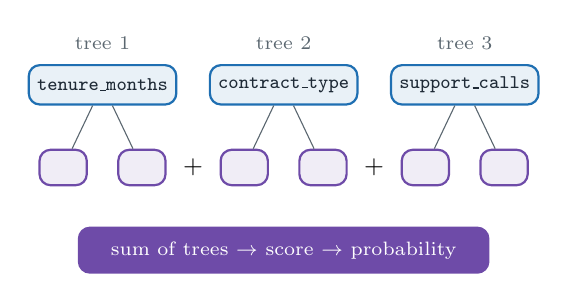
\begin{tikzpicture}[x=1cm,y=1cm,
          leaf/.style={cbox=cPurple,minimum width=0.6cm,minimum height=0.45cm,inner sep=1pt},
          nd/.style={cbox=cBlue,font=\scriptsize\ttfamily,minimum height=0.5cm,inner xsep=3pt,inner ysep=2pt}]
        \foreach \x/\t/\f/\i in {0/tree 1/tenure\_months/1,2.3/tree 2/contract\_type/2,4.6/tree 3/support\_calls/3}{
          \node[nd] (r\i) at (\x,0) {\f};
          \node[leaf] (a\i) at (\x-0.5,-1.05) {};
          \node[leaf] (b\i) at (\x+0.5,-1.05) {};
          \draw[cGray] (r\i) -- (a\i); \draw[cGray] (r\i) -- (b\i);
          \node[font=\scriptsize,text=cGray,anchor=base] at (\x,0.45) {\t};}
        \node[font=\small] at (1.15,-1.05) {+};
        \node[font=\small] at (3.45,-1.05) {+};
        \node[sbox=cPurple,font=\scriptsize,minimum width=5.2cm] at (2.3,-2.1) {sum of trees $\rightarrow$ score $\rightarrow$ probability};
      \end{tikzpicture}
    \end{column}
  \end{columns}
  \source{Chen \& Guestrin (2016); Grinsztajn et al.\ (2022)}
  \note{XGBoost (Chen \& Guestrin, KDD 2016) is an efficient implementation of gradient boosting: an ensemble of shallow decision trees, built sequentially so that each tree fits the remaining errors. Its ``sparsity-aware split finding'' learns a default direction for missing values -- no imputation needed.\par
  Grinsztajn, Oyallon and Varoquaux (NeurIPS 2022) showed on a large benchmark that tree-based models still outperform deep learning on typical tabular data -- which is exactly what most business data looks like (tables from ERP, CRM, finance).\par
  Feature importance (e.g. \texttt{model.feature\_importances\_}) gives a first, rough explanation of what drives predictions; it is not a causal statement. For individual explanations, methods like SHAP are used -- an extension for interested students. We do not derive the mathematics in this course.}
\end{frame}

% ------------------------------------------------------------------
\begin{frame}{Is the model any good?}{Accuracy alone can fool you}
  \vspace{2pt}
  \begin{columns}[T]
    \begin{column}{0.44\textwidth}
      \begin{badbox}[The accuracy trap]
        With 20\,\% churn, a ``model'' that always says \emph{no churn} is right 80\,\% of the time -- and useless.
      \end{badbox}
      \centering
      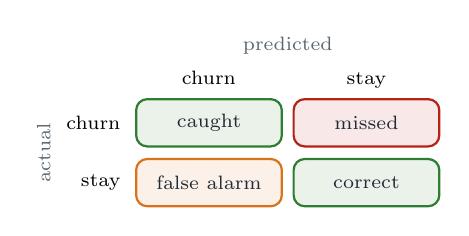
\begin{tikzpicture}[x=1cm,y=1cm,
          cmcell/.style={minimum width=1.85cm,minimum height=0.6cm,font=\scriptsize,inner sep=1pt}]
        \node[font=\scriptsize,text=cGray,anchor=base] at (2.55,1.3) {predicted};
        \node[font=\scriptsize,text=cGray,rotate=90] at (-0.55,0.0) {actual};
        \node[font=\scriptsize,anchor=base] at (1.55,0.87) {churn}; \node[font=\scriptsize,anchor=base] at (3.55,0.87) {stay};
        \node[font=\scriptsize,anchor=east] at (0.55,0.38) {churn}; \node[font=\scriptsize,anchor=east] at (0.55,-0.38) {stay};
        \node[cbox=cGreen,cmcell] at (1.55,0.38) {caught};
        \node[cbox=cRed,cmcell] at (3.55,0.38) {missed};
        \node[cbox=cOrange,cmcell] at (1.55,-0.38) {false alarm};
        \node[cbox=cGreen,cmcell] at (3.55,-0.38) {correct};
      \end{tikzpicture}
    \end{column}
    \begin{column}{0.52\textwidth}
      {\footnotesize
      \renewcommand{\arraystretch}{1.25}
      \begin{tabularx}{\linewidth}{@{}l Y@{}}
        \toprule
        \textbf{Metric} & \textbf{Question it answers}\\
        \midrule
        Precision & Of the customers we call, how many would really leave?\\
        Recall & Of all real churners, how many do we catch?\\
        ROC-AUC & How well does the score rank churners above stayers? (0.5 = random)\\
        Baseline & What does ``always no churn'' achieve?\\
        \bottomrule
      \end{tabularx}}
    \end{column}
  \end{columns}
  \takeaway{A missed churner costs a customer, a false alarm a discount -- \mbox{the threshold is a business decision.}}
  \note{This slide is where business students can outperform pure technicians. With imbalanced classes, accuracy is misleading: the majority-class baseline (scikit-learn's \texttt{DummyClassifier(strategy="most\_frequent")}) already reaches 80\% with 20\% churn. Always report the baseline next to the model.\par
  Tie the metrics to the matrix: recall = caught $\div$ (caught + missed), precision = caught $\div$ (caught + false alarms); the threshold is the probability above which we count a customer as ``churn'' and call them. Precision and recall describe the two kinds of error in the confusion matrix; ROC-AUC measures how well the probability ranks churners above non-churners across all thresholds (1.0 perfect, 0.5 random). The prompt therefore asks the training script to print accuracy, ROC-AUC, precision, recall and the dummy baseline.\par
  Business framing: the threshold (e.g. call everyone above 0.6) is a management decision based on the cost of a missed churner versus the cost of a retention offer -- not a technical default of 0.5.}
\end{frame}

% ------------------------------------------------------------------
\begin{frame}{POC 3 architecture}
  \centering
  \begin{tikzpicture}[x=1cm,y=1cm]
    \node[comp=cBlue,minimum height=2.05cm] (st) at (0,0) {\faChartBar\\[2pt]\textbf{Streamlit}\\\scriptsize frontend \textbullet\ 8501};
    \node[comp=cTeal,minimum height=2.05cm] (api) at (5.3,0) {\faServer\\[2pt]\textbf{FastAPI}\\\scriptsize backend \textbullet\ 8000};
    \node[comp=cPurple,minimum height=2.05cm,minimum width=3.3cm,text width=3.1cm] (ml) at (10.9,0) {\faBrain\\[2pt]\textbf{XGBoost}\\\scriptsize \texttt{model.json}\\loaded once at start};
    \node[comp=cOrange,minimum width=3.6cm,text width=3.4cm] (db) at (5.3,-2.5) {\faDatabase\ \ \textbf{SQLite}\\\scriptsize customers, predictions,\\\scriptsize model runs};
    \draw[darr] (st) -- node[lbl,above]{HTTP} node[lbl,below]{JSON} (api);
    \draw[darr] (api) -- node[lbl,above=2pt]{\texttt{predict\_proba}} (ml);
    \draw[darr] (api) -- node[lbl,right=2pt]{SQLAlchemy} (db);
  \end{tikzpicture}
  \par\vspace{4pt}
  \begin{infobox}[Data flow of one prediction]
    Streamlit $\rightarrow$ \mbox{\texttt{POST /api/predict}} $\rightarrow$ FastAPI builds the feature vector $\rightarrow$ model returns a probability $\rightarrow$ row in \texttt{predictions} $\rightarrow$ JSON back $\rightarrow$ Streamlit shows the score.
  \end{infobox}
  \note{The backend loads the model once at start-up in the lifespan function -- FastAPI's own documentation uses exactly this example (loading an ML model) for lifespan events. Loading the model on every request would be slow and wasteful.\par
  Walk through the data flow: the frontend sends the customer's features as JSON; FastAPI validates them with Pydantic, builds the same one-hot columns as in training (using the stored column list), calls \texttt{predict\_proba}, stores the prediction with a timestamp and the model-run ID, and returns the probability.\par
  Point out that the frontend still knows nothing about XGBoost. If the data-science team replaces the model tomorrow, the frontend does not change -- the API contract stays the same.}
\end{frame}

% ------------------------------------------------------------------
\begin{frame}[fragile]{POC 3: project structure}
  \vspace{2pt}
  \begin{columns}[T]
    \begin{column}{0.60\textwidth}
\begin{lstlisting}[basicstyle=\ttfamily\scriptsize,aboveskip=0pt]
poc3_xgboost_churn/
|-- .venv/
|-- backend/
|   |-- __init__.py
|   |-- main.py            # FastAPI app + endpoints
|   |-- models.py          # SQLAlchemy tables
|   |-- schemas.py         # Pydantic models
|   |-- database.py        # engine + session
|   |-- generate_data.py   # synthetic churn data
|   |-- train_model.py     # training + evaluation
|   |-- model.json         # trained XGBoost model
|   +-- model_meta.json    # feature columns, metrics
|-- frontend/app.py        # Streamlit UI
|-- data/customers.csv     # generated
|-- app.db                 # generated (ignored)
+-- requirements.txt
\end{lstlisting}
    \end{column}
    \begin{column}{0.36\textwidth}
      \begin{keybox}[New files]
        \file{generate\_data.py}, \file{train\_model.py}, \file{model.json}, \file{model\_meta.json}
      \end{keybox}
      \vspace{2pt}
      \begin{warnbox}[Training--serving skew]
        The backend must build \emph{exactly} the columns the model was trained on -- hence \file{model\_meta.json}.
      \end{warnbox}
    \end{column}
  \end{columns}
  \note{Compared to POC 2, the backend gets two scripts (data generation and training) and two artefacts (the model and its metadata). Training is a separate step, run once before starting the API -- or later via \texttt{POST /api/train}.\par
  The model is saved with XGBoost's \texttt{save\_model} as JSON rather than with pickle/joblib, following the XGBoost documentation's recommendation for long-term storage; the one-hot column list and the metrics go into a small JSON metadata file.\par
  ``Training--serving skew'' is a classic production bug: if the backend one-hot-encodes a request differently from training, the model receives different inputs. With pandas DataFrames XGBoost usually complains loudly (feature-name mismatch) -- the dangerous case is silent: a misspelled category such as ``Monthly'' becomes all zeros after reindexing. Reindexing to the stored column list plus strict category types (\texttt{Literal}) prevents both -- the backend prompt asks for it.}
\end{frame}

% ------------------------------------------------------------------
\begin{frame}{POC 3: API endpoints and tables}
  \vspace{2pt}
  {\footnotesize
  \renewcommand{\arraystretch}{1.28}
  \begin{tabularx}{\textwidth}{@{}l l Y@{}}
    \toprule
    \textbf{Method} & \textbf{Path} & \textbf{Purpose}\\
    \midrule
    \pill[cBlue]{GET} & \texttt{/api/customers}, \texttt{/api/customers/\{id\}} & list / details of stored customers\\
    \pill[cTeal]{POST} & \texttt{/api/predict} & prediction for a feature vector (JSON)\\
    \pill[cTeal]{POST} & \texttt{/api/predict/\{customer\_id\}} & prediction for a stored customer\\
    \pill[cBlue]{GET} & \texttt{/api/sample-customer} & a random example profile for testing\\
    \pill[cTeal]{POST} & \texttt{/api/train} & retrain the model (optional)\\
    \pill[cBlue]{GET} & \texttt{/api/model/info}, \texttt{/api/predictions} & model metrics; prediction history\\
    \bottomrule
  \end{tabularx}}
  \par\vspace{6pt}
  {\footnotesize
  \begin{tabularx}{\textwidth}{@{}l Y@{}}
    \toprule
    \textbf{Table} & \textbf{Columns (example)}\\
    \midrule
    \texttt{customers} & \texttt{id, age, contract\_type, tenure\_months, monthly\_charges, payment\_method, support\_calls, churn}\\
    \texttt{predictions} & \texttt{id, customer\_id, probability, prediction, model\_run\_id, created\_at}\\
    \texttt{model\_runs} & \texttt{id, trained\_at, n\_samples, accuracy, roc\_auc, precision, recall, model\_path}\\
    \bottomrule
  \end{tabularx}}
  \note{The API extends POC 2's pattern: GET for reading customers, model information and history; POST for predictions and retraining. \texttt{/api/sample-customer} plays the same role as \texttt{/api/sample} in POC 2 -- it makes testing possible without typing a full feature vector.\par
  The three tables make every prediction traceable: which customer, which probability, which model run, when. The model-run table stores the evaluation metrics of each training, so that a retrained model can be compared with the previous one before it is used.\par
  In business terms, this is a minimal ``model registry'' and ``prediction log'' -- concepts that MLOps platforms offer at scale.}
\end{frame}

% ------------------------------------------------------------------
\begin{frame}{POC 3: steps in agent mode}
  \vspace{4pt}
  \begin{columns}[T]
    \begin{column}{0.55\textwidth}
      \begin{enumerate}\setlength{\itemsep}{4pt}
        \item Repo root open; create \file{poc3\_xgboost\_churn/}; own \file{.venv}, activated and selected
        \item \textbf{Data \& model:} prompt 1 -- run training, read the metrics, \textbf{commit}
        \item \textbf{Backend:} prompt 2 (\texttt{/plan} $\rightarrow$ Implement Plan) -- test in \texttt{/docs}, \textbf{commit}
        \item \textbf{Frontend:} prompt 3 -- start both processes, test, \textbf{commit}
        \item Iterate: feature importance, threshold, batch scoring
      \end{enumerate}
    \end{column}
    \begin{column}{0.41\textwidth}
      \begin{keybox}[Checkpoint after step 2]
        Does the model beat the ``always no churn'' baseline? If not, fix the data before building an API.
      \end{keybox}
      \vspace{2pt}
      \begin{infobox}[Reuse]
        Tell the agent: ``Use the same structure and conventions as \file{poc2\_fastapi\_sqlite}.''
      \end{infobox}
    \end{column}
  \end{columns}
  \note{Three prompts, three commits. The order data $\rightarrow$ model $\rightarrow$ API $\rightarrow$ UI is the natural order of every ML application; each stage is tested before the next one is built.\par
  The checkpoint after step 2 is a professional habit: there is no point in building an API for a model that is not better than a trivial rule. Students should look at the printed metrics and compare ROC-AUC and recall with the baseline.\par
  The reuse tip is powerful with coding agents: pointing to an existing folder gives the agent a concrete template for structure and style -- the result is more consistent than a description from scratch.}
\end{frame}

% ------------------------------------------------------------------
\begin{frame}{POC 3: prompt 1 -- data and model}
  \vspace{2pt}
  \begin{promptbox}
    Work only inside \texttt{poc3\_xgboost\_churn/} and use its existing \texttt{.venv}. Create \texttt{backend/generate\_data.py}: generate a realistic synthetic churn dataset with numpy (about 5,000 rows; fields \texttt{id, age, tenure\_months, monthly\_charges, contract\_type, payment\_method, support\_calls, churn}; churn rate about 20\,\%, plausibly related to the features) and save it as \texttt{data/customers.csv}.
    Create \texttt{backend/train\_model.py}: run the generator if the CSV is missing; one-hot encode the categorical columns with pandas; stratified 80/20 split; train an \texttt{XGBClassifier}; print accuracy, ROC-AUC, precision, recall and the baseline of always predicting ``no churn''.
    Save the model with \texttt{save\_model("backend/model.json")} and the feature columns plus metrics to \texttt{backend/model\_meta.json}. Use package imports (\texttt{backend.generate\_data}). Create \texttt{requirements.txt} (numpy, pandas, scikit-learn, xgboost), install it and run \mbox{\texttt{python -m backend.train\_model}}. Done when the metrics are printed and \texttt{model.json} exists.
  \end{promptbox}
  \note{The prompt fixes the data schema, the churn rate and the relationship between features and target, so that the model has something to learn. Asking for ``plausibly related'' features typically yields rules like: short tenure, monthly contracts and many support calls increase the churn probability.\par
  The evaluation line implements the previous slide: several metrics plus the baseline. Saving the column list and metrics to \texttt{model\_meta.json} prepares the backend (column alignment) and the \texttt{/api/model/info} endpoint.\par
  The package-import instruction makes the same code work both as a script (\texttt{python -m backend.train\_model}, run from the project folder) and when the backend imports it for \texttt{POST /api/train}. After running it, discuss the output with the class: is ROC-AUC clearly above 0.5? Is recall acceptable? If the synthetic relationships are too strong, metrics look unrealistically perfect -- a good opportunity to discuss that real data is messier.}
\end{frame}

% ------------------------------------------------------------------
\begin{frame}{POC 3: prompt 2 -- backend}
  \vspace{2pt}
  \begin{promptbox}[Prompt for Copilot \textendash\ /plan, then Implement Plan]
    Create the FastAPI backend in \texttt{poc3\_xgboost\_churn/backend/} with the same structure and conventions as \texttt{poc2\_fastapi\_sqlite}. SQLAlchemy 2.0 models: Customer, Prediction, ModelRun.
    Endpoints: GET~\texttt{/api/customers}, GET~\texttt{/api/customers/\{id\}}, POST~\texttt{/api/predict}, POST~\texttt{/api/predict/\{customer\_id\}}, GET~\texttt{/api/sample-customer}, POST~\texttt{/api/train}, GET~\texttt{/api/model/info}, GET~\texttt{/api/predictions}.
    In a lifespan function: create the tables, import \texttt{data/customers.csv} if the customers table is empty, load \texttt{model.json} and \texttt{model\_meta.json} once, and create a ModelRun from the metadata if none exists. For each prediction, build the one-hot columns exactly as in \texttt{model\_meta.json}, store the prediction with the model run and return \texttt{churn\_probability}, \texttt{prediction} and \texttt{model\_run\_id}. \mbox{\texttt{POST /api/train}} adds a new ModelRun and reloads the model. Use \texttt{Literal[...]} for the categories. No CORS middleware. Add \texttt{fastapi[standard]} and \texttt{sqlalchemy} to \texttt{requirements.txt} and install them. Done when every endpoint works in \texttt{/docs}.
  \end{promptbox}
  \note{Key elements of this prompt: (1) reuse of the POC 2 conventions, (2) the complete endpoint list as the contract, (3) start-up work in the lifespan function -- creating tables, seeding customers and loading the model once, (4) the explicit column alignment against \texttt{model\_meta.json}, which prevents training--serving skew, and (5) logging every prediction with its model run.\par
  Two details avoid classic bugs: the ModelRun created from the metadata (training runs before the database exists), and \texttt{Literal} types for \texttt{contract\_type} and \texttt{payment\_method}, so that an unknown or misspelled category returns 422 instead of a silently wrong prediction. In the plan review, check that the agent loads the model with XGBoost's \texttt{load\_model} (not pickle), that the model is loaded once and not per request, and that predictions are written to the database.\par
  Test in \texttt{/docs}: call \texttt{/api/sample-customer}, copy the JSON into \texttt{/api/predict}, then check \texttt{/api/predictions}.}
\end{frame}

% ------------------------------------------------------------------
\begin{frame}{POC 3: prompt 3 -- frontend}
  \vspace{2pt}
  \begin{promptbox}
    In \texttt{poc3\_xgboost\_churn/}, create \texttt{frontend/app.py} (Streamlit, calls the backend only via HTTP, \texttt{BACKEND\_URL} as in POC 2) with three tabs:
    \par\smallskip
    \textbf{Customers:} table from GET~\texttt{/api/customers} with a filter by \texttt{contract\_type}.
    \par\smallskip
    \textbf{Prediction:} a form with all features and sensible defaults, a button ``Load sample customer'' (GET~\texttt{/api/sample-customer} fills the form) and a selectbox ``Choose existing customer'' (POST~\texttt{/api/predict/\{customer\_id\}}). The button ``Predict'' calls POST~\texttt{/api/predict} and shows the probability as a metric and a progress bar.
    \par\smallskip
    \textbf{History:} the latest predictions from GET~\texttt{/api/predictions}, plus the model metrics from GET~\texttt{/api/model/info}.
    \par\smallskip
    Add streamlit and requests to \texttt{requirements.txt} and install them. Done when all three tabs work with the sample customer.
  \end{promptbox}
  \note{One detail goes beyond a plain prediction form: the History tab also shows the model metrics, so users see how good the model is next to its predictions -- a small step towards transparency.\par
  The ``Load sample customer'' button uses the testing endpoint, so that students can try the app without typing values. \texttt{st.tabs}, \texttt{st.metric} and \texttt{st.progress} are standard Streamlit elements; the progress bar takes a value between 0.0 and 1.0 -- exactly a probability.\par
  Ask students to try extreme profiles (new customer, monthly contract, many support calls vs. long-term two-year contract) and check whether the probabilities move in the expected direction.}
\end{frame}

% ------------------------------------------------------------------
\begin{frame}{POC 3: run and verify}{Sanity checks for an ML app}
  \vspace{2pt}
  \begin{columns}[T]
    \begin{column}{0.50\textwidth}
      {\small\bfseries\color{cNavy}Model}\par\vspace{3pt}
      {\small
      \checkline{ROC-AUC clearly above 0.5; recall reported}
      \checkline{model beats the ``always no churn'' baseline}
      \checkline{\texttt{/api/model/info} shows the metrics}}
      \par\vspace{4pt}
      {\small\bfseries\color{cNavy}Behaviour}\par\vspace{3pt}
      {\small
      \checkline{high-risk profile $\rightarrow$ high probability}
      \checkline{loyal two-year customer $\rightarrow$ low probability}}
    \end{column}
    \begin{column}{0.46\textwidth}
      {\small\bfseries\color{cNavy}System}\par\vspace{3pt}
      {\small
      \checkline{every prediction appears in the history}
      \checkline{invalid input in \texttt{/docs} (text as age) \mbox{$\rightarrow$ 422, no crash}}
      \checkline{restart: model and data still there}}
      \par\vspace{6pt}
      \begin{warnbox}[Too good to be true?]
        ROC-AUC near 1.0 on synthetic data usually means the generator made churn too predictable.
      \end{warnbox}
    \end{column}
  \end{columns}
  \note{These checks combine the three levels of an ML application: model quality, plausible behaviour, and system behaviour. The behaviour checks are a simple form of what practitioners call ``invariance'' or ``directional'' tests: changing a feature in a known direction should move the prediction in the expected direction.\par
  Invalid input should never crash the backend: Pydantic returns 422 with a clear message. Persistence: after a restart, the model is loaded again from \texttt{model.json}, and the history is still in SQLite.\par
  The warning box addresses a typical surprise with synthetic data: if the generator uses deterministic rules, the model can learn them perfectly. Suggest adding noise to the generator -- and discuss why real churn is much harder to predict.}
\end{frame}

% ------------------------------------------------------------------
\begin{frame}{From prediction to action}{A score is not a decision}
  \vspace{2pt}
  \begin{columns}[T]
    \begin{column}{0.315\textwidth}
      \begin{card}[cTeal]{\faUserCheck\ \ Who acts?}[equal height group=act]
        The model ranks; people decide whom to contact and with which offer. Define the process around the score.
      \end{card}
    \end{column}
    \begin{column}{0.315\textwidth}
      \begin{card}[cBlue]{\faBalanceScale\ \ Fair \& explainable?}[equal height group=act]
        Would the model treat groups unfairly? Can we explain a score to a manager or a customer?
      \end{card}
    \end{column}
    \begin{column}{0.315\textwidth}
      \begin{card}[cOrange]{\faShield*\ \ Data protection}[equal height group=act]
        Real customer data is personal data: purpose limitation, access control, deletion -- GDPR applies.
      \end{card}
    \end{column}
  \end{columns}
  \takeaway{Automation creates value only when the prediction is embedded in a responsible business process.}
  \note{Close the technical part of POC 3 with the business perspective. A churn score is useful only if someone acts on it: which threshold triggers a call, who makes the call, which offer is allowed, how success is measured (e.g. with a control group).\par
  Fairness and explainability: our model even uses age directly -- a characteristic protected under the German General Equal Treatment Act (AGG). Ask the students whether it should be used at all. Features that correlate with protected characteristics can disadvantage groups too; feature importance and individual explanations help to detect this. For customer-facing decisions, companies must be able to explain the logic.\par
  Data protection: our data is synthetic. With real customer data, the GDPR principles (purpose limitation, data minimisation, access control, deletion) and internal policies apply -- a POC with real data therefore needs the data-protection officer early. The LLM deck returns to governance and the EU AI Act.}
\end{frame}

% ------------------------------------------------------------------
\begin{frame}{POC 3: extensions}
  \vspace{4pt}
  \begin{columns}[T]
    \begin{column}{0.48\textwidth}
      \begin{card}[cBlue]{\pill[cTeal]{EASY}\ \ Quick wins}[equal height group=ext3]
        \begin{itemize}\setlength{\itemsep}{2pt}
          \item feature-importance chart in the History tab
          \item threshold slider: who gets called?
          \item colour the probability \mbox{(green / amber / red)}
        \end{itemize}
      \end{card}
    \end{column}
    \begin{column}{0.48\textwidth}
      \begin{card}[cPurple]{\pill[cOrange]{HARDER}\ \ Closer to reality}[equal height group=ext3]
        \begin{itemize}\setlength{\itemsep}{2pt}
          \item batch scoring: upload a CSV, download scores
          \item compare two model runs before~switching
          \item train on the IBM Telco churn dataset
        \end{itemize}
      \end{card}
    \end{column}
  \end{columns}
  \takeaway{Batch scoring is how churn models are used in practice: a nightly list for the sales team.}
  \note{The extensions move the POC towards real usage. The threshold slider makes the business trade-off tangible: moving it shows how many customers would be contacted and how many churners would be caught (on the test data).\par
  Batch scoring -- upload a customer list, get scores back -- is the typical production pattern for churn models: a scheduled job scores all customers overnight and hands a prioritised list to sales or marketing. Combined with an automation tool, that list could trigger retention workflows automatically.\par
  Comparing model runs before switching introduces the idea of model governance: a new model is only deployed if it is demonstrably better on the same test data.}
\end{frame}
% ==================================================================
% PART 8 -- WRAP-UP
% ==================================================================
\section{Wrap-up}
\partframe{Session 2 and following}{What you built, what is still missing -- and what comes next.}{%
  \darkitem{Compare the three architectures at a glance}
  \darkitem{Know what separates a POC from a product}
  \darkitem{Take seven habits into every future project}}

% ------------------------------------------------------------------
\begin{frame}{Three POCs at a glance}
  \centering
  \begin{tikzpicture}[x=1cm,y=1cm]
    % POC 1
    \node[lab] at (0,0) {POC 1};
    \node[bx=cBlue,minimum width=1.1cm] (u1) at (2.6,0) {\faUser};
    \node[bx=cBlue,minimum width=2.1cm] (s1) at (4.9,0) {Streamlit};
    \node[bx=cGray,minimum width=2.6cm] (m1) at (8.1,0) {data in memory};
    \draw[arr] (u1) -- (s1); \draw[arr] (s1) -- (m1);
    % POC 2
    \node[lab] at (0,-1.3) {POC 2};
    \node[bx=cBlue,minimum width=1.1cm] (u2) at (2.6,-1.3) {\faUser};
    \node[bx=cBlue,minimum width=2.1cm] (s2) at (4.9,-1.3) {Streamlit};
    \node[bx=cTeal,minimum width=2.1cm] (a2) at (7.8,-1.3) {FastAPI};
    \node[bx=cOrange,minimum width=2.1cm] (d2) at (10.7,-1.3) {SQLite};
    \draw[arr] (u2) -- (s2); \draw[arr] (s2) -- (a2); \draw[arr] (a2) -- (d2);
    % POC 3
    \node[lab] at (0,-2.6) {POC 3};
    \node[bx=cBlue,minimum width=1.1cm] (u3) at (2.6,-2.6) {\faUser};
    \node[bx=cBlue,minimum width=2.1cm] (s3) at (4.9,-2.6) {Streamlit};
    \node[bx=cTeal,minimum width=2.1cm] (a3) at (7.8,-2.6) {FastAPI};
    \node[bx=cOrange,minimum width=2.1cm] (d3) at (10.7,-2.6) {SQLite};
    \node[bx=cPurple,minimum width=2.1cm] (x3) at (7.8,-3.65) {XGBoost};
    \draw[arr] (u3) -- (s3); \draw[arr] (s3) -- (a3); \draw[arr] (a3) -- (d3); \draw[arr] (a3) -- (x3);
    % annotations
    \node[font=\scriptsize,text=cGray,anchor=west] at (12.0,0) {one process};
    \node[font=\scriptsize,text=cGray,anchor=west] at (12.0,-1.3) {+ API, + database};
    \node[font=\scriptsize,text=cGray,anchor=west] at (12.0,-2.6) {+ model layer};
  \end{tikzpicture}
  \takeaway{Each stage \emph{adds} to the architecture -- nothing is taken away.}
  \note{Use this summary diagram to let the students retell the journey in their own words. POC 1: one process, everything in memory. POC 2: the same functionality, but with an API and a database -- persistence, reuse, separation. POC 3: the same architecture plus a model layer -- data, model, API and UI together form a small ML product.\par
  Question for the audience: ``Which of the three would you choose for (a) a one-off data exploration, (b) an internal tool used by ten colleagues, (c) a churn score that the CRM system should use every night?'' Answers: (a) POC 1, (b) POC 2, (c) POC 3 -- and for (c) the API would be called by the CRM or an automation workflow, not only by Streamlit.}
\end{frame}

% ------------------------------------------------------------------
\begin{frame}{From POC to production}{What we deliberately left out -- but a product needs}
  \vspace{2pt}
  {\footnotesize
  \renewcommand{\arraystretch}{1.3}
  \begin{tabularx}{\textwidth}{@{}l Y L{4.3cm}@{}}
    \toprule
    \textbf{Topic} & \textbf{What a product needs} & \textbf{Who usually owns it}\\
    \midrule
    \makebox[1.6em][l]{\faVial}Tests & automated tests for logic and API & development team\\
    \makebox[1.6em][l]{\faLock}Access & login, roles, permissions & IT / security\\
    \makebox[1.6em][l]{\faCloud}Deployment & servers or cloud, backups, updates & IT operations\\
    \makebox[1.6em][l]{\faHeartbeat}Monitoring & errors, performance, model drift & operations / data science\\
    \makebox[1.6em][l]{\faShield*}Data protection & GDPR, data minimisation, deletion & data-protection officer\\
    \makebox[1.6em][l]{\faUsers}Ownership & who maintains and pays for it? & business owner\\
    \bottomrule
  \end{tabularx}}
  \takeaway{A POC answers \emph{whether} it works. Production answers \emph{how} it keeps working -- safely.}
  \note{Return to the question from Part 1: what would be missing before the finance department could use the expense-claim checker with real data? This table is the structured answer. Each row is a whole discipline, which is why POCs should be handed over to professionals once the idea is proven -- or rebuilt properly.\par
  Model drift deserves a sentence: the churn model was trained on past data; if customer behaviour changes (new competitor, new tariffs), its predictions get worse without any error message. Monitoring the model's performance over time is therefore part of operating an ML application.\par
  The ``ownership'' row is the most underestimated one in practice: many good prototypes die because nobody is responsible for them after the project ends.}
\end{frame}

% ------------------------------------------------------------------
\begin{frame}{Seven take-aways}
  \vspace{2pt}
  \begin{columns}[T]
    \begin{column}{0.53\textwidth}
      \begin{enumerate}\setlength{\itemsep}{5pt}\small
        \item \textbf{POC = learning speed over robustness.} Three~small apps beat one perfect project.
        \item \textbf{AI-assisted coding is a loop.} Describe, generate, review, test, commit.
        \item \textbf{Prompt quality = code quality.} Goal, stack, files, interfaces, demo data, done-criteria.
        \item \textbf{Read it, run it, check it.} Only then commit it.
      \end{enumerate}
    \end{column}
    \begin{column}{0.46\textwidth}
      \begin{enumerate}\setcounter{enumi}{4}\setlength{\itemsep}{5pt}\small
        \item \textbf{Architecture is ``who calls whom, how''} -- the use case can stay the same.
        \item \textbf{ML app = three tiers + a model layer} -- and the right metrics.
        \item \textbf{Secrets never go into Git.} \texttt{.gitignore} before the first commit.
      \end{enumerate}
    \end{column}
  \end{columns}
  \takeaway{You now own a professional toolchain -- and three prototypes that prove you can use it.}
  \note{Summarise the seven habits. Invite students to pick the one they found most surprising -- typically ``prompt quality equals code quality'' or ``architecture is who calls whom''.\par
  Link to the next deck: everything the Copilot agent did in these sessions -- planning, calling tools, reading results, iterating -- is an instance of agentic AI. The LLM deck explains how large language models, retrieval-augmented generation and agents work, and uses the same AI-assisted coding method for three LLM prototypes (chat with your PDF, semantic product search, a ShopCo support agent).\par
  Recommended follow-up task: write a one-page reflection on one POC -- what worked, what the agent got wrong, and how you noticed.}
\end{frame}

% ------------------------------------------------------------------
\begin{frame}{Resources}
  \vspace{2pt}
  \begin{keybox}[\faGithub\ \ Course repository]
    \href{https://github.com/ChrisW09/Python-for-AI-Driven-Automation}{\texttt{github.com/ChrisW09/Python-for-AI-Driven-Automation}}\\
    \footnotesize From your first line of Python to AI-driven automation: notebooks, exercises, data and slides.
  \end{keybox}
  \vspace{2pt}
  \begin{columns}[T]
    \begin{column}{0.60\textwidth}
      \tcbset{equal height group=res105}%
      \begin{graybox}[Documentation]
        \vspace{2pt}{\footnotesize
        \begin{tabular}{@{}l@{\hspace{5pt}}l@{}}
          VS Code AI & \href{https://code.visualstudio.com/docs/agents/overview}{\texttt{code.visualstudio.com/docs}}\\
          GitHub Copilot & \href{https://docs.github.com/copilot}{\texttt{docs.github.com/copilot}}\\
          Streamlit & \href{https://docs.streamlit.io}{\texttt{docs.streamlit.io}}\\
          FastAPI & \href{https://fastapi.tiangolo.com}{\texttt{fastapi.tiangolo.com}}\\
          SQLAlchemy & \href{https://docs.sqlalchemy.org}{\texttt{docs.sqlalchemy.org}}\\
          XGBoost & \href{https://xgboost.readthedocs.io}{\texttt{xgboost.readthedocs.io}}\\
          Git book & \href{https://git-scm.com/book}{\texttt{git-scm.com/book}}\\
        \end{tabular}}
      \end{graybox}
    \end{column}
    \begin{column}{0.36\textwidth}
      \tcbset{equal height group=res105}%
      \begin{graybox}[Further reading]
        {\small Simon Willison's blog on AI-assisted programming: \href{https://simonwillison.net}{\texttt{simonwillison.net}}\par\vspace{3pt}
        MDN Web Docs on HTTP:\\\href{https://developer.mozilla.org/en-US/docs/Web/HTTP}{\texttt{developer.mozilla.org}}\par\vspace{3pt}
        Outlook: React, Vue, Svelte -- frontend frameworks for products, not used here.}
      \end{graybox}
    \end{column}
  \end{columns}
  \note{Point to the course repository first: it is the home of the module's materials -- Jupyter notebooks from Python basics to AI engineering, exercises with solutions, sample data and the slides. Students who are new to Python start with the onboarding and foundations modules. All documentation links are official sources and were checked in early October 2026. The VS Code and GitHub Copilot documentation changes frequently -- whenever the students' screens differ from the slides, the docs are the reference.\par
  The Git book (Pro Git, by Scott Chacon and Ben Straub) is available free online, also in German (\texttt{git-scm.com/book/de}).\par
  Simon Willison's blog is one of the most careful practitioner sources on using LLMs for programming, including the distinction between vibe coding and responsible AI-assisted development that we used in Part 1.}
\end{frame}

% ------------------------------------------------------------------
\begin{frame}{References}
  \vspace{2pt}
  {\scriptsize
  \refitem{Becker, J., Rush, N., Barnes, E., \& Rein, D. (2025). Measuring the impact of early-2025 AI on experienced open-source developer productivity. arXiv:2507.09089.}
  \refitem{Chen, T., \& Guestrin, C. (2016). XGBoost: A Scalable Tree Boosting System. \emph{Proc.\ KDD '16}, 785--794.}
  \refitem{Dell'Acqua, F., et al.\ (2026). Navigating the jagged technological frontier: Field experimental evidence of the effects of artificial intelligence on knowledge worker productivity and quality. \emph{Organization Science} 37(2), 403--423.}
  \refitem{Fielding, R.\ T.\ (2000). \emph{Architectural styles and the design of network-based software architectures}. PhD dissertation, University of California, Irvine.}
  \refitem{Grinsztajn, L., Oyallon, E., \& Varoquaux, G.\ (2022). Why do tree-based models still outperform deep learning on typical tabular data? \emph{NeurIPS 35} (Datasets \& Benchmarks).}
  \refitem{Karpathy, A.\ (2025, 2 Feb). ``There's a new kind of coding I call `vibe coding' \ldots'' [Post on X]. \url{https://x.com/karpathy/status/1886192184808149383}}
  \refitem{Noy, S., \& Zhang, W.\ (2023). Experimental evidence on the productivity effects of generative artificial intelligence. \emph{Science} 381(6654), 187--192.}
  \refitem{Peng, S., Kalliamvakou, E., Cihon, P., \& Demirer, M.\ (2023). The impact of AI on developer productivity: Evidence from GitHub Copilot. arXiv:2302.06590.}
  \refitem{Willison, S.\ (2025, 19 Mar). Not all AI-assisted programming is vibe coding (but vibe coding rocks). \url{https://simonwillison.net/2025/Mar/19/vibe-coding/}}}
  \note{All references were checked against the primary sources in September 2026. Note on Dell'Acqua et al.: the study circulated as Harvard Business School Working Paper 24-013 (2023) and was published in Organization Science in 2026; the published version reports a quality improvement of about 32\% inside the frontier, lower than the ``more than 40\%'' often quoted from the working paper.\par
  Product documentation used for facts about GitHub Copilot, VS Code, Python, Streamlit, FastAPI, SQLite, SQLAlchemy and XGBoost is listed on the resources slide; these facts reflect the state of September 2026.}
\end{frame}

% ------------------------------------------------------------------
\begin{frame}[plain,noframenumbering]
  \begin{tikzpicture}[remember picture,overlay]
    \fill[cNavy] (current page.south west) rectangle (current page.north east);
    \fill[cTeal] ($(current page.west)+(0.65,1.3)$) rectangle ++(1.4,-0.07);
    \node[anchor=north west,text=white,font=\fontsize{30}{32}\selectfont\bfseries,inner sep=0pt] at ($(current page.west)+(0.65,1.0)$) {Questions?};
    \node[anchor=north west,text=white!80!cTeal,font=\normalsize,text width=9.8cm,align=left,inner sep=0pt] at ($(current page.west)+(0.65,-0.2)$) {Next: LLMs, RAG \& Agentic AI -- the building blocks of \mbox{AI-driven} automation};
    \node[anchor=north west,text=white,font=\small,inner sep=0pt] at ($(current page.west)+(0.65,-1.55)$) {{\color{cTeal!70!white}\faEnvelope}\ \ christoph.weisser@hsbi.de};
    \node[anchor=north west,text=white,font=\small,inner sep=0pt] at ($(current page.west)+(0.65,-2.05)$) {{\color{cTeal!70!white}\faGithub}\ \ {\hypersetup{urlcolor=white}\href{https://github.com/ChrisW09/Python-for-AI-Driven-Automation}{github.com/ChrisW09/Python-for-AI-Driven-Automation}}};
    \node[anchor=north west,text=white!70,font=\footnotesize,inner sep=0pt,align=left] at ($(current page.west)+(0.65,-2.75)$) {Prof.\ Dr.\ Christoph Weisser\\[1pt] AI-Driven Automation \textbullet\ Bielefeld School of Business, HSBI};
    \begin{scope}[shift={($(current page.south east)+(-3.4,2.2)$)}]
      \foreach \x/\y/\n in {0/0/a,1.4/0.9/b,-0.9/1.6/c,0.6/2.6/d,2.2/2.2/e,-1.6/0.2/f,1.9/-0.6/g,-0.3/-1.2/h,0.9/1.6/i}
        {\coordinate (\n) at (\x,\y);}
      \foreach \u/\v in {a/b,a/c,a/f,a/h,b/e,b/g,b/i,c/d,c/i,d/e,d/i,e/i,f/c,g/h,a/i}
        {\draw[white,opacity=0.18,line width=0.6pt] (\u) -- (\v);}
      \foreach \n in {a,b,c,d,e,f,g,h,i}{\fill[cTeal!80!white] (\n) circle (2.2pt);}
      \fill[cOrange] (i) circle (3pt);
    \end{scope}
  \end{tikzpicture}
  \note{Open the floor for questions. Useful prompts if the room is quiet: ``Where did the agent surprise you -- positively or negatively?'', ``Which business process from your internship would you prototype next?''\par
  Point once more to the course repository for practice material. Remind students to push their final POC versions to GitHub before the next session and to keep their Copilot setup ready for the LLM prototypes.}
\end{frame}
\end{document}
